\chapter{Discussion} \label{chapter:Discussion}

% \newcommand{\IMfitChiSquare}{1077.4}
\newcommand{\IMfitNDF}{352}
\newcommand{\IMfitChiNDF}{3.06}

\newcommand{\KzeroFitChi}{275.2}
\newcommand{\KzeroFitNDF}{43}
\newcommand{\KzeroFitChiNDF}{6.40}

\newcommand{\KzeroOneStepRatio}{80.9 \pm 1.3\%}
\newcommand{\KzeroTwoStepRatio}{11.5 \pm 1.0\%}
\newcommand{\KzeroLsRatio}{7.7 \pm 0.6\%}


% \section{Template fitting of $K^- d \rightarrow n \pi^+ \pi^- n$ events} \label{sec:tempFit}
% \subsection{Backward $\pi^{\mp}\Sigma^{\pm}$ event selection} \label{sec:backward_piSigma}
\begin{figure}
  \centering
  \begin{tikzpicture}[scale=1.2]
    \draw (-1.5,    1) node {$K^-$}--(0,    0);
    \draw (-1.5,    0)--(0,    0);
    \draw (-1.5, -0.2)--(0.3, -0.2);
    \node (d) at (-1.5, -0.1) [left] {$d$};

    \draw (0, 0) -- (0.3, -0.2) [dashed];
    \node (barK) at (0.3, -0.15) [above] {$\bar{K}$};

    \draw ( 1.5,  1.0) node [right] {\textcolor{red}{$n$ detected}}      -- (0,    0);
    
    \draw ( 1.5,  -0.7) node [right] {\textcolor{blue}{$\pi$ detected}} -- (0.3, -0.2);
    
    \draw ( 0.8,  -0.15) node [above] {$\Sigma$}    -- (0.3, -0.2);
    \draw ( 0.8,  -0.15) -- (1.5, 0.1) node [right] {$n$ missing};
    \draw ( 0.8,  -0.15) -- (1.5, -0.3) node [right] {\textcolor{blue}{$\pi$ detected}};    
  \end{tikzpicture}\\
  (a)
  
  \begin{tabular}{cc}
    \begin{minipage}{0.5\hsize}
      \centering
      \begin{tikzpicture}[scale=1.2]
        \draw (-1.5,    1) node {$K^-$}--(0,    0);
        \draw (-1.5,    0)--(0,    0);
        \draw (-1.5, -0.2)--(0, -0.2);
        \node (d) at (-1.5, -0.1) [left] {$d$};
        
        \draw ( 1.5,  1.0) node [right] {\textcolor{red}{$n$ detected}}      -- (0,    0);

        
        \node (K0) at (0.5, -0.4) [below] {$K^0$};
        \draw (0, -0.1) -- (0.7, -0.45);
        
        \draw ( 0.0,  -0.15) -- (1.5, 0.1) node [right] {$n$ missing};
        \draw ( 0.7,  -0.45) -- (1.5, -0.3) node [right] {\textcolor{blue}{$\pi$ detected}};
        \draw (1.5,  -0.7) node [right] {\textcolor{blue}{$\pi$ detected}} -- (0.7, -0.45);
        
        \filldraw [fill=white] (0, -0.1) circle [radius=0.15];
      \end{tikzpicture}\\
      (b)
    \end{minipage}
    \begin{minipage}{0.5\hsize}
      \centering
      \begin{tikzpicture}[scale=1.2]
        \draw (-1.5,    1) node {$K^-$}--(0,    0);
        \draw (-1.5,    0)--(0,    0);
        \draw (-1.5, -0.2)--(0.3, -0.2);
        \node (d) at (-1.5, -0.1) [left] {$d$};

        \draw ( 1.5,  -0.2) node [right] {n missing} -- (0.3, -0.2);
        \draw ( 1.5,  0.3) node [right] {\textcolor{blue}{$\pi$ detected}}      -- (0,    0);

        \node (barK) at (0.4, 0.4) [above] {$\Sigma$};
        \draw ( 0.7,  0.6) -- (0.0, 0.0);
                
        \draw ( 0.7,  0.6) -- (1.5, 1.5) node [right] {\textcolor{red}{$n$ detected}};
        \draw ( 0.7,  0.6) -- (1.5, 1.0) node [right] {\textcolor{blue}{$\pi$ detected}};    
      \end{tikzpicture}\\
      (c)
    \end{minipage}
  \end{tabular}
  \label{fig:kd_npipin_type}
\end{figure}


The $K^- n \rightarrow n \pi^+ \pi^- n$ final state is identified from the event in which the forward neutron is detected,
as described in Section.\ref{sec:???}.
This final state can be considered to include the three reactions represented in Figure \ref{fig:kd_npipin_type}.
The first is the signal reaction in this analysis where $\bar{K}$ is recoiled backward to $\pi \Sigma$
as shown in Figure.\ref{fig:kd_npipin_type}-(a),
the second is the recoil of $K^0$ decaying directly to $\pi^+ \pi^-$ as shown in Figure \ref{fig:kd_npipin_type}-(b),
and the third is the forward production of $\Sigma$ ($\Sigma_{forward}$) as shown in Figure \ref{fig:kd_npipin_type}-(c),
where forward means that the $n$ decaying from $\Sigma$ are detected by the NC.
Reactions (b) and (c) can be identified by reconstructing $K^0$ and $\Sigma^{\pm}$
from the invariant masses of $\pi^+$ and $\pi^-$ and forward neutrons and $\pi^{\pm}$, respectively,
as shown in Figure.\ref{fig:npipin_IM_fitGauss}.
The invariant mass distributions of $\pi^+ \pi^-$, $n \pi^-$ and $n \pi^+$ are represented in the right, center and left figures respectively.
For the identification of $K^0$ and $\Sigma^{\pm}_{forward}$,
fitting with third-order polynomial function and Gaussian function is used to identify $K^0$ and $\Sigma^{\pm}_{forward}$
in the 3$\sigma$ region of the Gaussian function, which is indicated by the red hatched area.

\begin{figure}[htbp]
  \begin{tabular}{ccc}
    \begin{minipage}{0.33\hsize}
      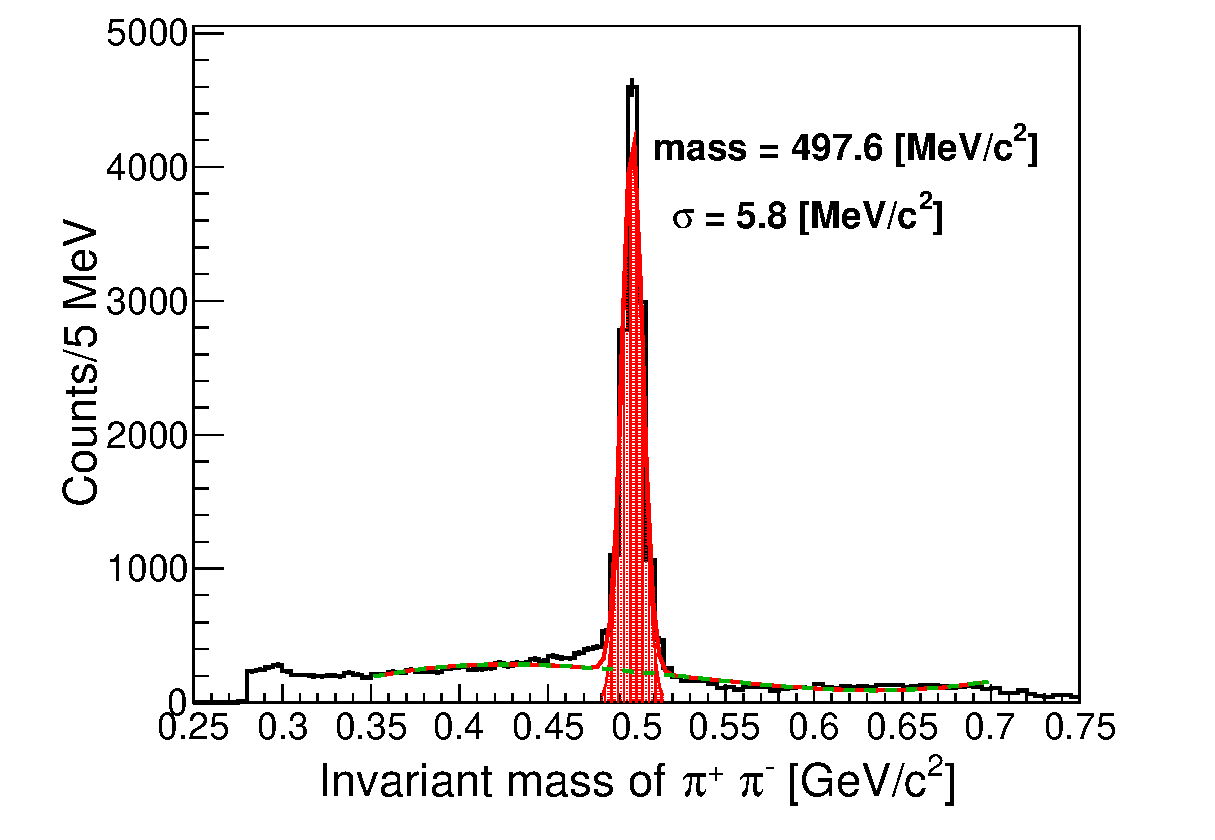
\includegraphics[width=4.5cm]{../pic/Run78/KN_ana_NC170_3sigma/IM_pipi_fitGauss.eps}
    \end{minipage}

    \begin{minipage}{0.33\hsize}
      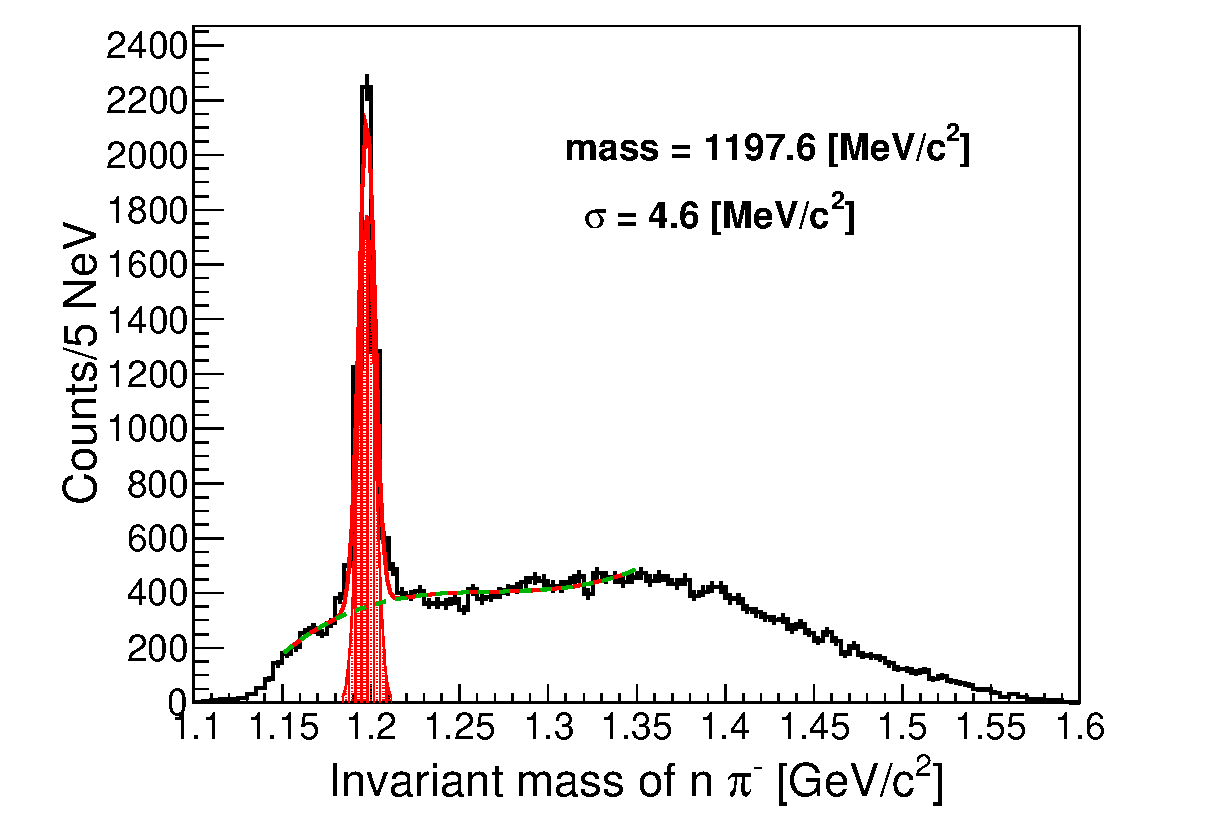
\includegraphics[width=4.5cm]{../pic/Run78/KN_ana_NC170_3sigma/IM_npim_fitGauss.eps}
    \end{minipage}

    \begin{minipage}{0.33\hsize}
      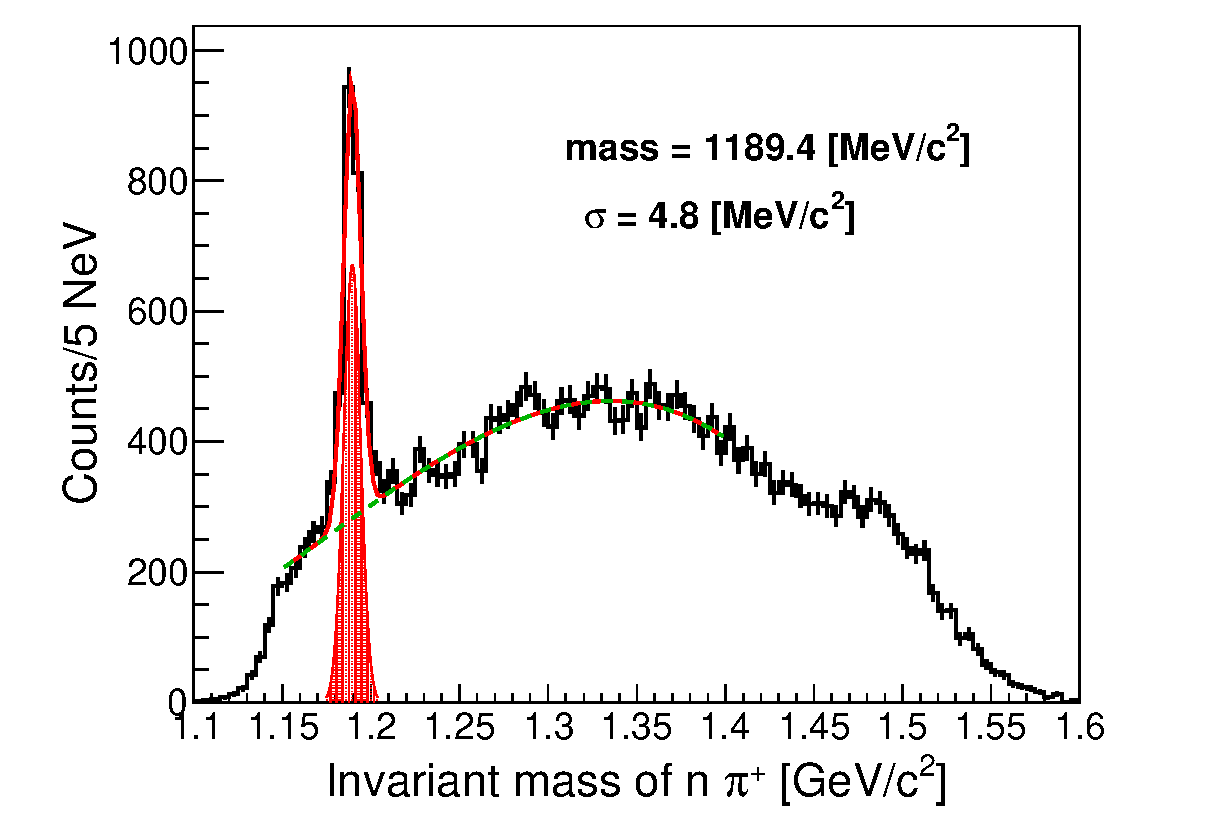
\includegraphics[width=4.5cm]{../pic/Run78/KN_ana_NC170_3sigma/IM_npip_fitGauss.eps}
    \end{minipage}
  \end{tabular}
  \caption{
    These figures show the invariant mass distributions of $\pi^+ \pi^-$,
    $n \pi^-$ and $n \pi^+$ in the $K d \rightarrow n \pi^+ \pi^- n$ event sample from left to right.
    The Gaussian functions and the selection regions for $K^0$ and $\Sigma^{\pm}_{forward}$ are indicated by red hatched area.
    The background third-order polynomial functions are shown as the green dashed lines.
  }
  \label{fig:npipin_IM_fitGauss}
\end{figure}


Rejecting these two reactions leaves a signal reaction in which $\pi \Sigma$ is scattered backward.
This reaction has $\pi^- \Sigma^+$ and $\pi^+ \Sigma^-$ modes, and they must be separated.
The branching ratio of these modes depends on the mass of $\pi \Sigma$, and this separation is performed for each bin of $d(K^-, n)$ missing mass.

\begin{frame}{$d(K^-, n)"nK0"$}
  \begin{figure}
    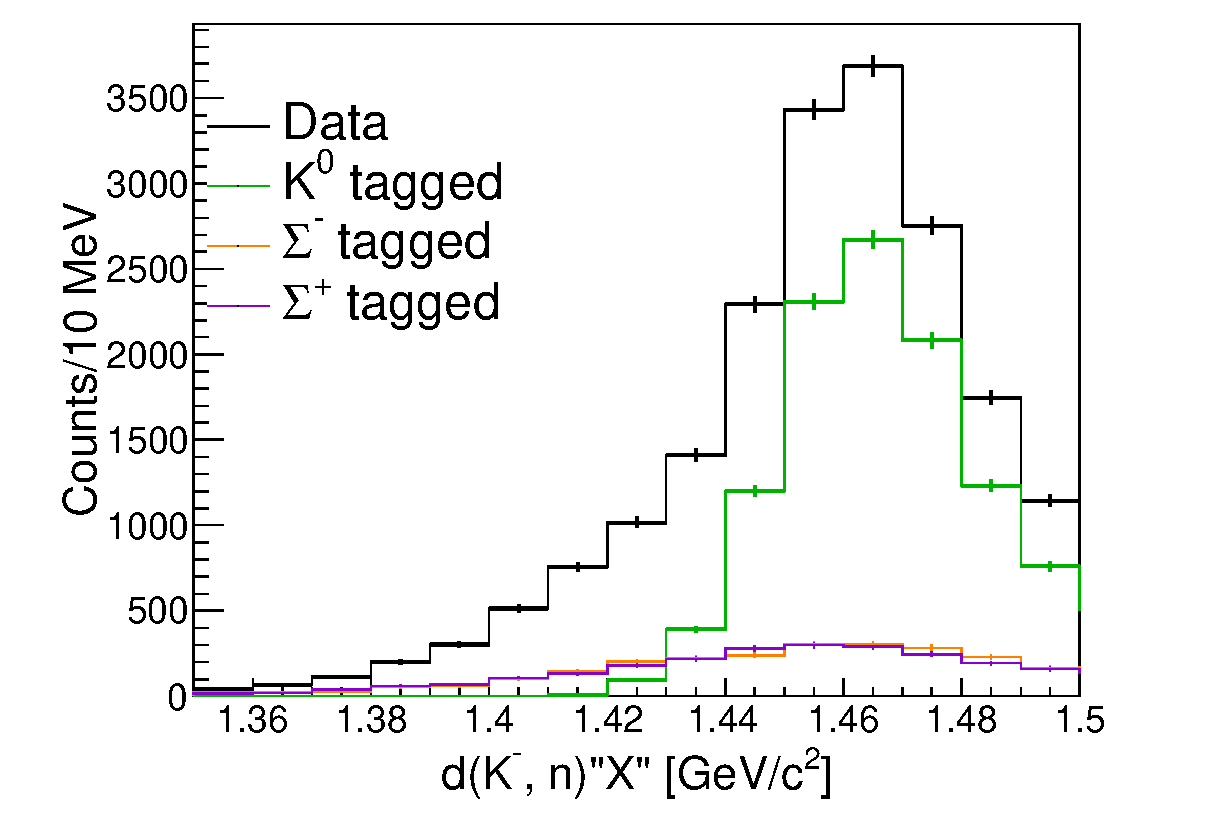
\includegraphics[width=8cm]{../pic/Run78/KN_ana_NC170_2sigma/KN_MM_all.eps}
  \end{figure}
\end{frame}


Figure \ref{fig:KN_MM_npipin} shows the $d(K^-, n)$ missing masses in which the $K^- d \rightarrow n \pi^+ \pi^- n$ final state has been identified.
On the left, all events, those identifying $K^0$, those identifying $\Sigma^+_{forward}$, and those identifying $\Sigma^-_{forward}$
are indicated by black, green, red, and blue lines, respectively.
The right figure shows the signal spectrum, subtracting the events identified as $K^0$ or $\Sigma^{\pm}_{forward}$ from all events.

To separate these events,
we generated template events using a Geant4 Monte Carlo simulation and decomposed the reactions by fitting their spectra with templates.
This decomposition was applied not only to the signal but also to the background reactions.
The procedures used in this decomposition are described in detail in Section \ref{sec:template_fitting}
The estimation of the detector resolution used in this simulation is described in detail in Appendix \ref{chapter:detector_resolution}.



\subsection{Template fitting} \label{sec:template_fitting}
\newcommand{\IMfitChiSquare}{1077.4}
\newcommand{\IMfitNDF}{352}
\newcommand{\IMfitChiNDF}{3.06}

\newcommand{\KzeroFitChi}{275.2}
\newcommand{\KzeroFitNDF}{43}
\newcommand{\KzeroFitChiNDF}{6.40}

\newcommand{\KzeroOneStepRatio}{80.9 \pm 1.3\%}
\newcommand{\KzeroTwoStepRatio}{11.5 \pm 1.0\%}
\newcommand{\KzeroLsRatio}{7.7 \pm 0.6\%}


% \section{Template fitting of $K^- d \rightarrow n \pi^+ \pi^- n$ events} \label{sec:tempFit}
% \subsection{Backward $\pi^{\mp}\Sigma^{\pm}$ event selection} \label{sec:backward_piSigma}
\input{analysis/template_fitting/figs/kd_npipin_type}

The $K^- n \rightarrow n \pi^+ \pi^- n$ final state is identified from the event in which the forward neutron is detected,
as described in Section.\ref{sec:???}.
This final state can be considered to include the three reactions represented in Figure \ref{fig:kd_npipin_type}.
The first is the signal reaction in this analysis where $\bar{K}$ is recoiled backward to $\pi \Sigma$
as shown in Figure.\ref{fig:kd_npipin_type}-(a),
the second is the recoil of $K^0$ decaying directly to $\pi^+ \pi^-$ as shown in Figure \ref{fig:kd_npipin_type}-(b),
and the third is the forward production of $\Sigma$ ($\Sigma_{forward}$) as shown in Figure \ref{fig:kd_npipin_type}-(c),
where forward means that the $n$ decaying from $\Sigma$ are detected by the NC.
Reactions (b) and (c) can be identified by reconstructing $K^0$ and $\Sigma^{\pm}$
from the invariant masses of $\pi^+$ and $\pi^-$ and forward neutrons and $\pi^{\pm}$, respectively,
as shown in Figure.\ref{fig:npipin_IM_fitGauss}.
The invariant mass distributions of $\pi^+ \pi^-$, $n \pi^-$ and $n \pi^+$ are represented in the right, center and left figures respectively.
For the identification of $K^0$ and $\Sigma^{\pm}_{forward}$,
fitting with third-order polynomial function and Gaussian function is used to identify $K^0$ and $\Sigma^{\pm}_{forward}$
in the 3$\sigma$ region of the Gaussian function, which is indicated by the red hatched area.

\input{analysis/template_fitting/figs/npipin_IM_fitGauss}

Rejecting these two reactions leaves a signal reaction in which $\pi \Sigma$ is scattered backward.
This reaction has $\pi^- \Sigma^+$ and $\pi^+ \Sigma^-$ modes, and they must be separated.
The branching ratio of these modes depends on the mass of $\pi \Sigma$, and this separation is performed for each bin of $d(K^-, n)$ missing mass.

\input{analysis/template_fitting/figs/KN_MM}

Figure \ref{fig:KN_MM_npipin} shows the $d(K^-, n)$ missing masses in which the $K^- d \rightarrow n \pi^+ \pi^- n$ final state has been identified.
On the left, all events, those identifying $K^0$, those identifying $\Sigma^+_{forward}$, and those identifying $\Sigma^-_{forward}$
are indicated by black, green, red, and blue lines, respectively.
The right figure shows the signal spectrum, subtracting the events identified as $K^0$ or $\Sigma^{\pm}_{forward}$ from all events.

To separate these events,
we generated template events using a Geant4 Monte Carlo simulation and decomposed the reactions by fitting their spectra with templates.
This decomposition was applied not only to the signal but also to the background reactions.
The procedures used in this decomposition are described in detail in Section \ref{sec:template_fitting}
The estimation of the detector resolution used in this simulation is described in detail in Appendix \ref{chapter:detector_resolution}.



\subsection{Template fitting} \label{sec:template_fitting}
\input{discussion/template_fitting/params}

% \section{Template fitting of $K^- d \rightarrow n \pi^+ \pi^- n$ events} \label{sec:tempFit}
% \subsection{Backward $\pi^{\mp}\Sigma^{\pm}$ event selection} \label{sec:backward_piSigma}
\input{discussion/template_fitting/backward_piSigma_selection}

\subsection{Template fitting} \label{sec:template_fitting}
\input{discussion/template_fitting/template_fitting}

%% \input{discussion/template_fitting/MC_data}
%% \input{discussion/template_fitting/procedure}
%% \input{discussion/template_fitting/fit_K0}



%% \subsection{Generated data by Monte Calro simulation} \label{subsec:tempFit_MCdata}
\input{discussion/template_fitting/reactions}
Since the $K^- d\rightarrow n \pi^+ \pi^- n$ event is expected to contain 3 type reactions, (\ref{reaction:prodK0})-(\ref{2step:piS}),
we obtain the $d(K^-, n)"\pi^{\mp}\Sigma^{\pm}"$ event rejecting $K^0$ and $\Sigma^{\pm}_{forward}$ in $K^- d \rightarrow n \pi^+ \pi^- n$ event.

We perform template fitting using data reproduced using Monte Carlo simulation (geant4) to decompose into $\pi^-\Sigma^+$ and $\pi^+\Sigma^-$ modes.
In this subsection, we explain how we reproduce the data using geant4 simulation.

The $K^0$ production in (\ref{reaction:prodK0}) is simply the so-called quasi-elastic scattering,
in which an initial $K^-$ reacts with a proton and is converted into $K^0$ and a neutron, where the residual neutron is a spectator and its momentum is the Fermi momentum.
This reaction causes the scattering angles of the reacting protons and $K^-$ to be distributed in a way that reproduces the past experiment of one nucleon scattering \cite{KP_K0n},
and the momentum of the spectator is also distributed in a way that reproduces the past experiment \cite{d_fermi_ex}.
In the case of $\Sigma^{\pm}_{forward}$ production in (\ref{reaction:prodSigma}), the angular distribution of the past experiment\cite{KP_CEX_1GeV} is simulated in the same way.

In the $K^0$ produced event (\ref{reaction:prodK0}), in addition to 1-step reaction described above, events such as a 2-step and direct $\Lambda(1520)$ production are observed.
So, we generate data of these reaction.
In the case of 2-step reaction, the momentum of recoiled $\bar{K}$ is small and the scattering data of such $\bar{K}$ and nucleon are a few,
so the angular distribution and other details are not known.
Therefore, the MC data is generated assuming that the scattering of recoiled $\bar{K}$ and nucleons is isotropic. 
In the case of direct $\Lambda(1520)$ production also no data.
Therefore, this data was isotropically scattered $K^-d \rightarrow n \Lambda(1520)$ and $\Lambda(1520)$ decayed to $n$ and $K^0$.

Next, we explain the main signal (\ref{2step:piS}), which is the backward $\pi\Sigma$ generation.
Since there is no data on the invariant mass of $\pi\Sigma$, it is generated as a uniform distribution from the $\bar{K}N$ threshold, whose lineshape is determined by template fitting.
There is also no data on the scattering angle of $\pi\Sigma$,
but since the $\bar{K}N\rightarrow \pi\Sigma$ scattering is expected to be $S$-wave in this reaction,
we assume that it is isotropic and generate MC data.

In summary, the following seven MC data are used for template fitting.
\input{discussion/template_fitting/MC_data_list}

%% \subsection{Procedure of template fitting}
\input{discussion/template_fitting/figs/fit_IM}
\input{discussion/template_fitting/figs/fit_KNpi_MM_all}

In this subsection, we explain procedure of template fitting, whose main purpose is decomposition of $\pi^- \Sigma^+$ and $\pi^+ \Sigma^-$ modes.
Template fitting is divided into two stages, one fitting to estimate the amount of background for $K^0$ and $\Sigma_{forward}$ production,
the other to separate $\pi^-\Sigma^+$ and $\pi^+\Sigma^-$ modes.
These fittings are performed using fitting with the likelihood method on a finite sample generated by Monte Carlo method\cite{temp_fit}.
There is no $\chi^2$ in this fitting,
but there is a value of $-2\log\Lambda$ that asymptotically approaches the $\chi^2$ when the number of samples become infinite, and the fitting is evaluated with this value.
Here, $\Lambda$ is the likelihood.

The first fitting is performed using the invariant mass distributions of $\pi^+ \pi^-$, $n \pi^+$ and $n \pi^-$ in the event that $K^-d \rightarrow n \pi^+ \pi^- n$ final state.
The $K^0$, $\Sigma^+$ and $\Sigma^-$ productions create peaks in the respective invariant mass distributions as shown in Fig.\ref{fig:fit_IM}.
The distributions reconstructed by fitting are also plotted in the same figure.
The bold line represents the case of backward $\pi \Sigma$ production of signal, with red and blue representing the $\pi^- \Sigma^+$ and $\pi^-\Sigma^+$ modes, respectively.
The other green, purple and orange lines represent the background for $K^0$, $\Sigma^-_{forward}$ and $\Sigma^+_{forward}$ production, respectively.
This fitting of $-2\log\Lambda$ is \IMfitChiSquare.
Degrees freedom is the number of bin with data, and $-2\log\Lambda/NDF \sim $\IMfitChiNDF. 
% For this purpose, the distribution is fitted with a Gaussian and a 5-th polynomial function, and the rejection region is defined by the 3$\sigma$ of the Gaussian.

\input{discussion/template_fitting/figs/fit_KNpi_MM}
\input{discussion/template_fitting/figs/tempFit_KNpi_Chi2}

The fitting to separate the $\pi^-\Sigma^+$ and $\pi^+\Sigma^-$ modes is performed for events from $K^-- d \rightarrow n \pi^+ \pi- n$, excluding $K^0 $and $\Sigma^{\pm}_{forward}$ production.
However, the background leakage is estimated by scaling the distribution reconstructed in the MC simulation by the intensity estimated by the invariant mass fitting.
This fitting is performed each bin of the missing mass of $d(K^-, n)$, since the scattering amplitude of $\bar{K}N \rightarrow \pi \Sigma$ depends on the $\pi \Sigma$ invariant mass.
For this fitting we use the $d(K^-, n \pi^-)$ and $d(K^-, n \pi^+)$ missing masses as shown in Fig.\ref{fig:fit_KNpi_MM_all}.
This figure shows the sum of the $d(K^- , n)$ bins.
The bottom left figure shows a two-dimensional figure of the $d(K^-, n \pi^-)$ and $d(K^-, n \pi^+)$ missing masses on the horizontal and vertical axes, respectively.
The top and right figures show the projections of the respective axes.
The missing mass of $d(K^-, n \pi)$ makes a peak at $\Sigma$ for the correct combination for the missing $\Sigma$, but is widely distributed in the kinematic region for the opposite charge.
For example, for $d(K^-, n \pi^-)$, the $\pi^- \Sigma^+$ mode has a peak structure as shown by the red line,
whereas the $\pi^+ \Sigma^-$ mode has a widely distributed structure as shown by the blue line.

Fig.\ref{fig:fit_KNpi_MM} shows the results for the fitting of each bin of $d(K^-, n)$ separately.
Fig.\ref{fig:tempFit_KNpi_Chi2} shows the $-2\log\Lambda$ and $-2\log\Lambda/NDF$ of this fitting in each $d(K^-, n)$ bin in black and red, respectively.

Fitting to estimate background and to separate $\pi^- \Sigma^+$ and $\pi^+ \Sigma^-$ modes cannot be performed simultaneously as they use different event samples.
They are therefore repeated in the following steps.

First, the separation of $\pi^- \Sigma^+$ and $\pi^+ \Sigma^-$ modes is performed without considering the background.
The obtained distribution of backward $\pi^{\mp} \Sigma^{\pm}$ modes is used for fitting to estimate the background,
which is then fed back into the fitting of the separation of $\pi^- \Sigma^+$ and $\pi^+ \Sigma^-$ modes.
After five iterations of this procedure, fitting is performed considering 2-step and direct $\Lambda(1520)$ generation for $K^0$ generation, which is described in the Appendix.\ref{apendix:K0_event}.
Finally, fitting of the separation of the $\pi^- \Sigma^+$ and $\pi^+ \Sigma^-$ modes is performed to obtain the final $\pi \Sigma$ spectrum as shown in Fig.\ref{fig:piS_num}..

\input{discussion/template_fitting/figs/piS_num}


%% \begin{frame}{Template fitting to decompose $K^0$ production}
  \begin{figure}
    \centering
    Invariant mass of $n K^0$\\
    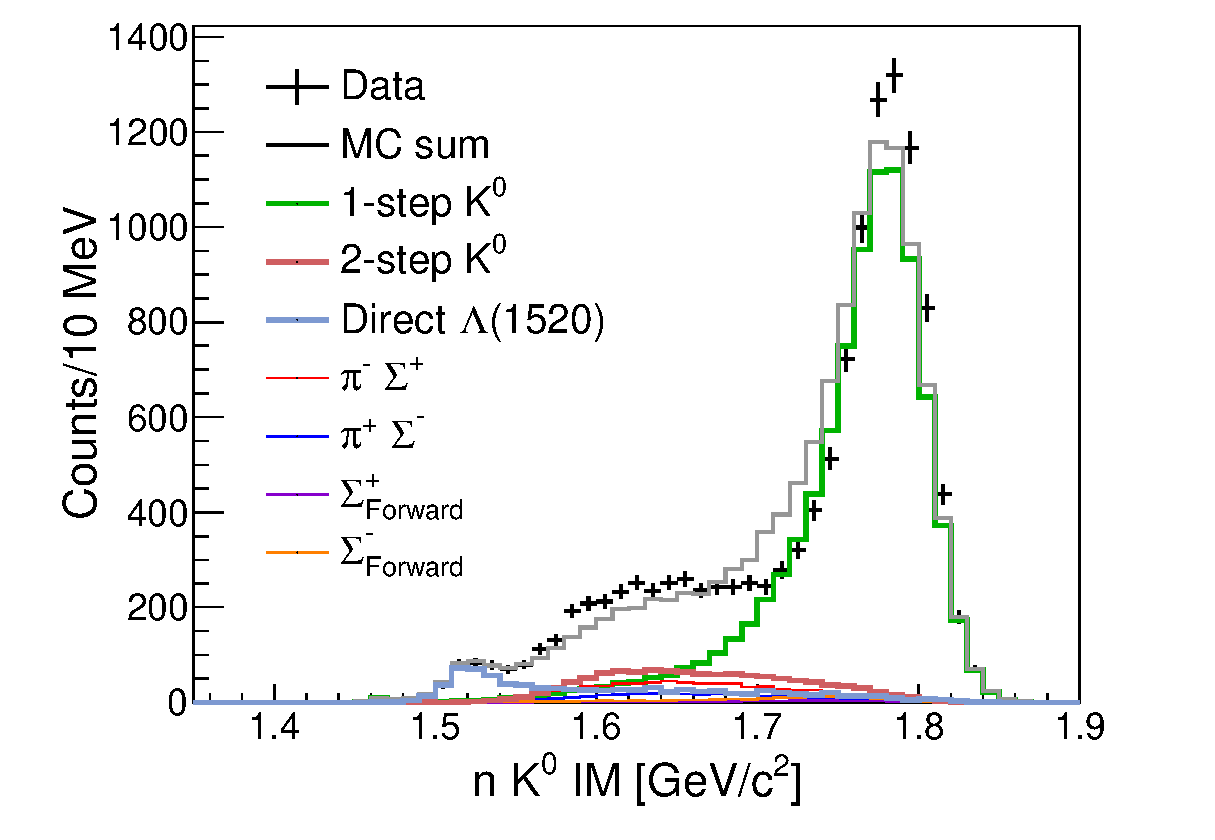
\includegraphics[width=7.5cm]{../pic/Dron/K0_ana/npipi_IM_K0.eps}
  \end{figure}
  \centering
  2-step like component is seen about 11.5\%.\\
  Direct-$\Lambda(1520)$ prod. is seen about 7.7\%.\\
\end{frame}




%% \subsection{Generated data by Monte Calro simulation} \label{subsec:tempFit_MCdata}
\begin{eqnarray}
  & &  K^- d \rightarrow n K^0 n \label{reaction:prodK0} \\
  & &  K^- d \rightarrow \pi^\mp \Sigma^\pm n_{forward} \label{2step:piS}\\
  & &  K^- d \rightarrow \pi^\mp \Sigma^\pm n_{missing} \label{reaction:prodSigma}
\end{eqnarray}

Since the $K^- d\rightarrow n \pi^+ \pi^- n$ event is expected to contain 3 type reactions, (\ref{reaction:prodK0})-(\ref{2step:piS}),
we obtain the $d(K^-, n)"\pi^{\mp}\Sigma^{\pm}"$ event rejecting $K^0$ and $\Sigma^{\pm}_{forward}$ in $K^- d \rightarrow n \pi^+ \pi^- n$ event.

We perform template fitting using data reproduced using Monte Carlo simulation (geant4) to decompose into $\pi^-\Sigma^+$ and $\pi^+\Sigma^-$ modes.
In this subsection, we explain how we reproduce the data using geant4 simulation.

The $K^0$ production in (\ref{reaction:prodK0}) is simply the so-called quasi-elastic scattering,
in which an initial $K^-$ reacts with a proton and is converted into $K^0$ and a neutron, where the residual neutron is a spectator and its momentum is the Fermi momentum.
This reaction causes the scattering angles of the reacting protons and $K^-$ to be distributed in a way that reproduces the past experiment of one nucleon scattering \cite{KP_K0n},
and the momentum of the spectator is also distributed in a way that reproduces the past experiment \cite{d_fermi_ex}.
In the case of $\Sigma^{\pm}_{forward}$ production in (\ref{reaction:prodSigma}), the angular distribution of the past experiment\cite{KP_CEX_1GeV} is simulated in the same way.

In the $K^0$ produced event (\ref{reaction:prodK0}), in addition to 1-step reaction described above, events such as a 2-step and direct $\Lambda(1520)$ production are observed.
So, we generate data of these reaction.
In the case of 2-step reaction, the momentum of recoiled $\bar{K}$ is small and the scattering data of such $\bar{K}$ and nucleon are a few,
so the angular distribution and other details are not known.
Therefore, the MC data is generated assuming that the scattering of recoiled $\bar{K}$ and nucleons is isotropic. 
In the case of direct $\Lambda(1520)$ production also no data.
Therefore, this data was isotropically scattered $K^-d \rightarrow n \Lambda(1520)$ and $\Lambda(1520)$ decayed to $n$ and $K^0$.

Next, we explain the main signal (\ref{2step:piS}), which is the backward $\pi\Sigma$ generation.
Since there is no data on the invariant mass of $\pi\Sigma$, it is generated as a uniform distribution from the $\bar{K}N$ threshold, whose lineshape is determined by template fitting.
There is also no data on the scattering angle of $\pi\Sigma$,
but since the $\bar{K}N\rightarrow \pi\Sigma$ scattering is expected to be $S$-wave in this reaction,
we assume that it is isotropic and generate MC data.

In summary, the following seven MC data are used for template fitting.
\begin{itemize}
  \item About $K^0$ production reaction
  \begin{itemize}
  \item
    $ K^- d \rightarrow n_{forward} K^0 n_{spectator}$ \hspace{\fill} ($K^0$ 1-step)
  \item
    $K^- d \rightarrow n_{forward} (K^0 n)_{isotropic}$ \hspace{\fill} ($K^0$ 2-step)
  \item
    $K^- d \rightarrow n \Lambda(1520) \rightarrow n K^0 n$ \hspace{\fill} (direct $\Lambda(1520)$)
  \end{itemize}
\item About $\Sigma_{forward}$ production reaction
  \begin{itemize}
  \item
    $K^- d \rightarrow \Sigma^+ \pi^- n_{spectator} \rightarrow n_{forward} \pi^+ \pi^- n_{spectator}$ \hspace{\fill} ($\Sigma^+$ 1-step)
  \item
    $K^- d \rightarrow \Sigma^- \pi^+ n_{spectator} \rightarrow n_{forward} \pi^- \pi^+ n_{spectator}$ \hspace{\fill} ($\Sigma^-$ 1-step)
  \end{itemize}
\item About backward $\pi \Sigma$ production reaction
  \begin{itemize}
  \item
    $K^- d \rightarrow n_{forward} \pi^- \Sigma^+$ \hspace{\fill} (backward $\pi^- \Sigma^+$)
  \item
    $K^- d \rightarrow n_{forward} \pi^+ \Sigma^-$ \hspace{\fill} (backward $\pi^+ \Sigma^-$)
  \end{itemize}
\end{itemize}


%% \subsection{Procedure of template fitting}
\begin{frame}{Template fitting to evaluate background}
  \centering
  $d(K^, n \pi^- \pi^+)"n"$ event.
  \begin{tabular}{ccc}
    \begin{minipage}{0.33\hsize}
      \centering
      $\pi^+ \pi^-$ IM\\
      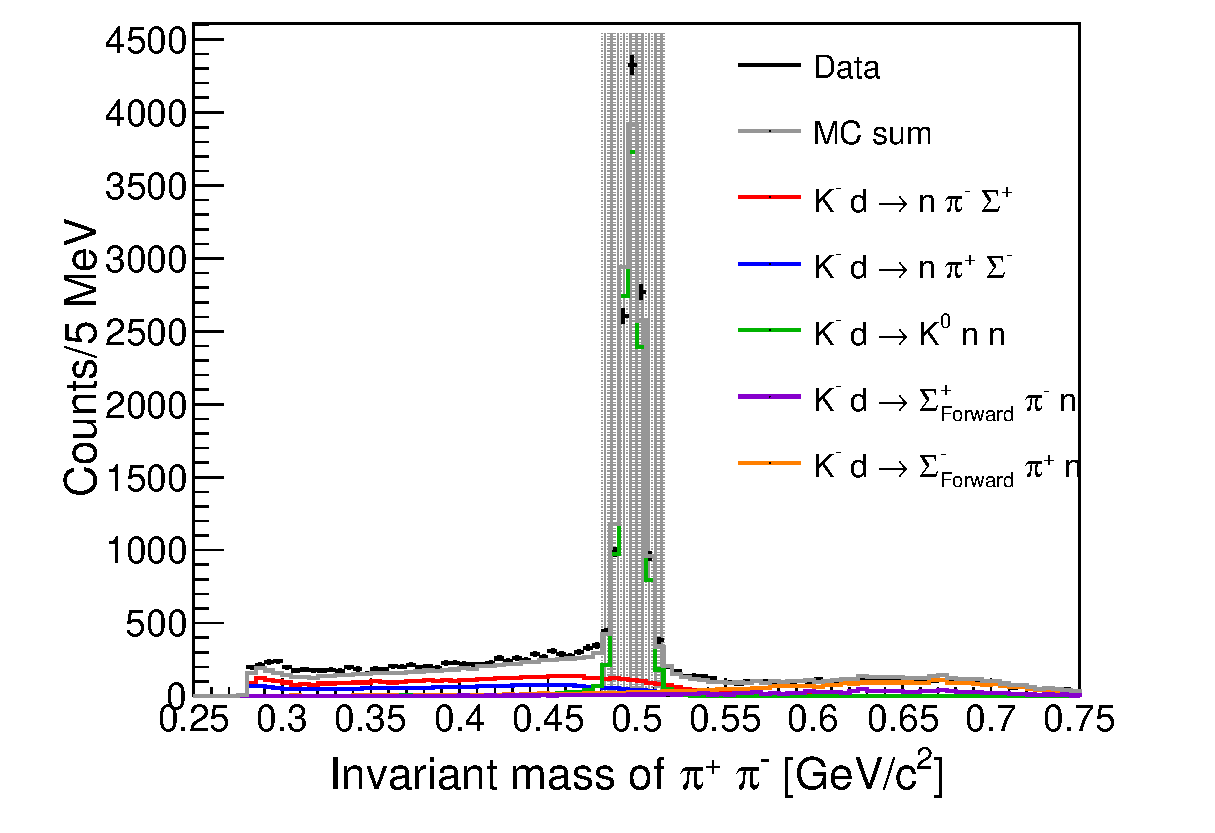
\includegraphics[width=4cm]{../pic/Dron/KN_ana/IM_pipi.eps}
    \end{minipage}
    \begin{minipage}{0.33\hsize}
      \centering
      $n_{forward} \pi^+$ IM\\
      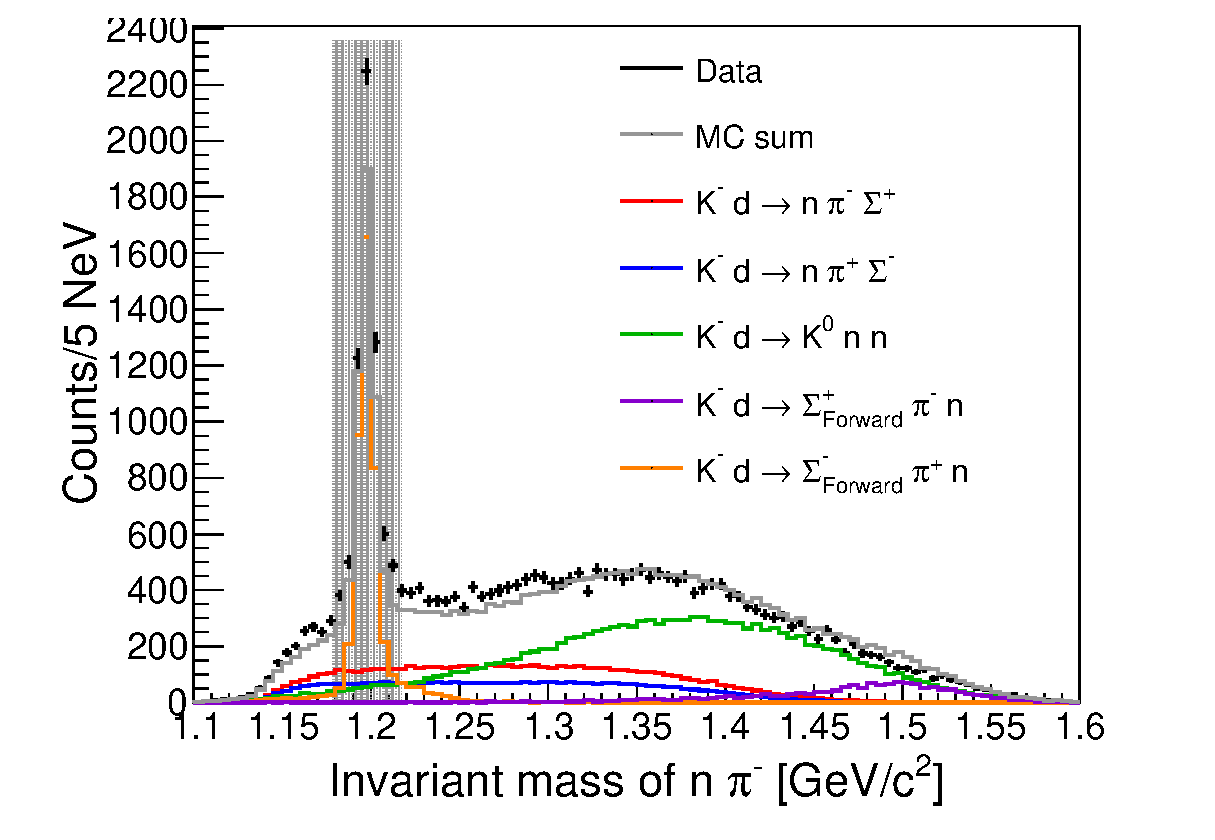
\includegraphics[width=4cm]{../pic/Dron/KN_ana/IM_npim.eps}
    \end{minipage}
    \begin{minipage}{0.33\hsize}
      \centering
      $n_{forward} \pi^-$ IM\\
      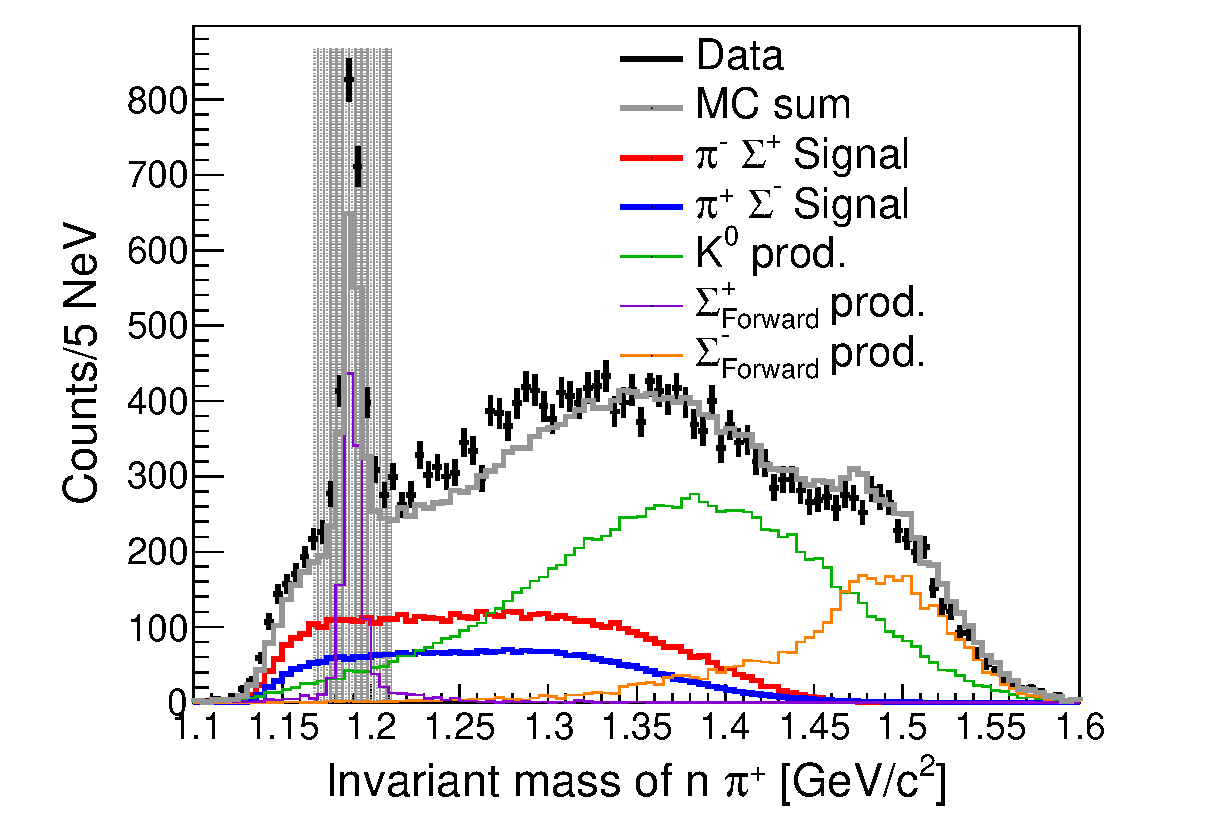
\includegraphics[width=4cm]{../pic/Dron/KN_ana/IM_npip.eps}
    \end{minipage}
  \end{tabular}
  \vspace{4mm}\\
  Each spectra are well reproduced. 
\end{frame}

\begin{figure}[htbp]
  \centering
  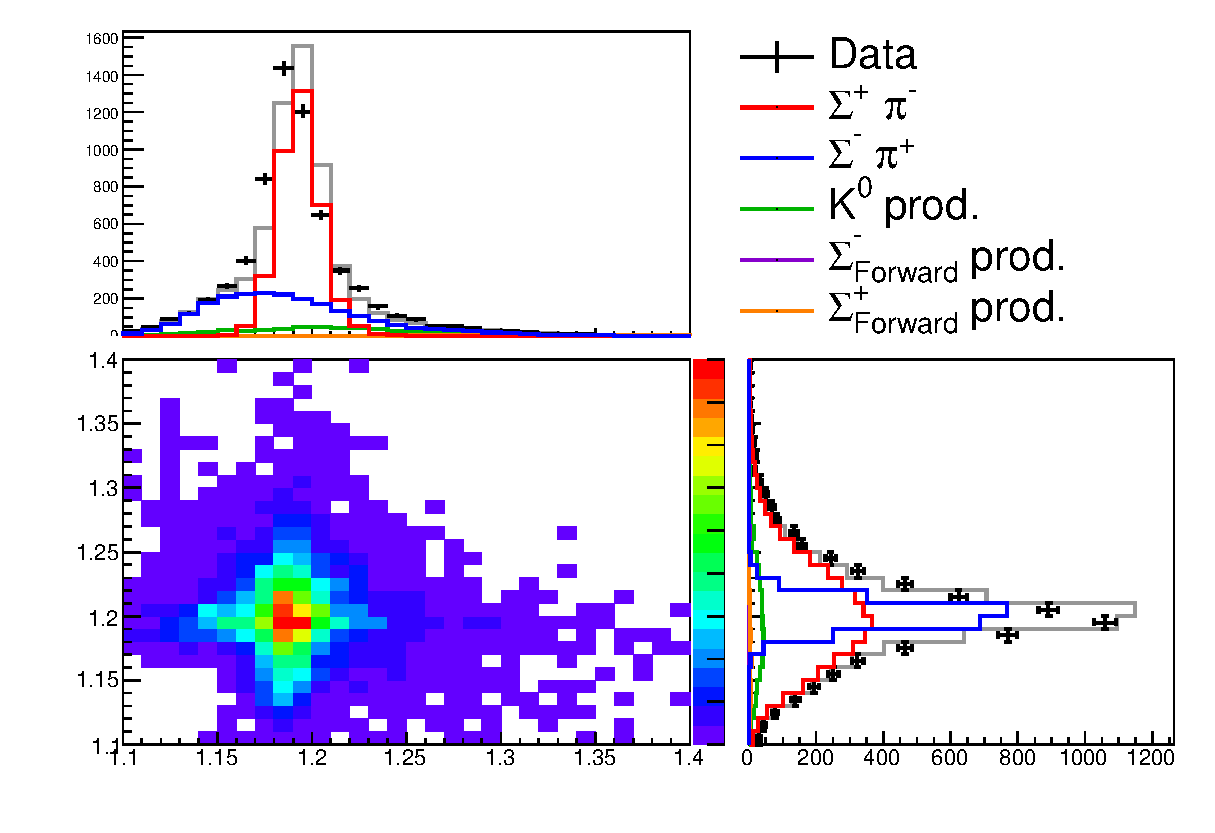
\includegraphics[width=12cm]{../pic/Run78/KN_ana_NC170_2sigma/KNpim_KNpip_MM.eps}
  \caption{
    This figure shows template fitting of the $d(K^-, n \pi)$ spectra to separate the $\pi^-\Sigma^+$ and $\pi^+ \Sigma^-$ modes.
    The lower left figure shows two-dimensional plots of $d(K^-, n \pi^-)$ and $d(K^-, n \pi^+)$ on the horizontal and vertical axes, respectively.
    The top and right panels show the projections onto each axis.
    The caption is the same as that of Figure.\ref{fig:fit_IM}.
  }
  \label{fig:fit_KNpi_MM_all}
\end{figure}


In this subsection, we explain procedure of template fitting, whose main purpose is decomposition of $\pi^- \Sigma^+$ and $\pi^+ \Sigma^-$ modes.
Template fitting is divided into two stages, one fitting to estimate the amount of background for $K^0$ and $\Sigma_{forward}$ production,
the other to separate $\pi^-\Sigma^+$ and $\pi^+\Sigma^-$ modes.
These fittings are performed using fitting with the likelihood method on a finite sample generated by Monte Carlo method\cite{temp_fit}.
There is no $\chi^2$ in this fitting,
but there is a value of $-2\log\Lambda$ that asymptotically approaches the $\chi^2$ when the number of samples become infinite, and the fitting is evaluated with this value.
Here, $\Lambda$ is the likelihood.

The first fitting is performed using the invariant mass distributions of $\pi^+ \pi^-$, $n \pi^+$ and $n \pi^-$ in the event that $K^-d \rightarrow n \pi^+ \pi^- n$ final state.
The $K^0$, $\Sigma^+$ and $\Sigma^-$ productions create peaks in the respective invariant mass distributions as shown in Fig.\ref{fig:fit_IM}.
The distributions reconstructed by fitting are also plotted in the same figure.
The bold line represents the case of backward $\pi \Sigma$ production of signal, with red and blue representing the $\pi^- \Sigma^+$ and $\pi^-\Sigma^+$ modes, respectively.
The other green, purple and orange lines represent the background for $K^0$, $\Sigma^-_{forward}$ and $\Sigma^+_{forward}$ production, respectively.
This fitting of $-2\log\Lambda$ is \IMfitChiSquare.
Degrees freedom is the number of bin with data, and $-2\log\Lambda/NDF \sim $\IMfitChiNDF. 
% For this purpose, the distribution is fitted with a Gaussian and a 5-th polynomial function, and the rejection region is defined by the 3$\sigma$ of the Gaussian.

\begin{figure}
  \begin{tabular}{ccccc}
    \begin{minipage}{0.2\hsize}
      \includegraphics[width=2.2cm]{../pic/Run78/KN_ana_NC170_2sigma/KNpi_MM_0.eps}
    \end{minipage}
    \begin{minipage}{0.2\hsize}
      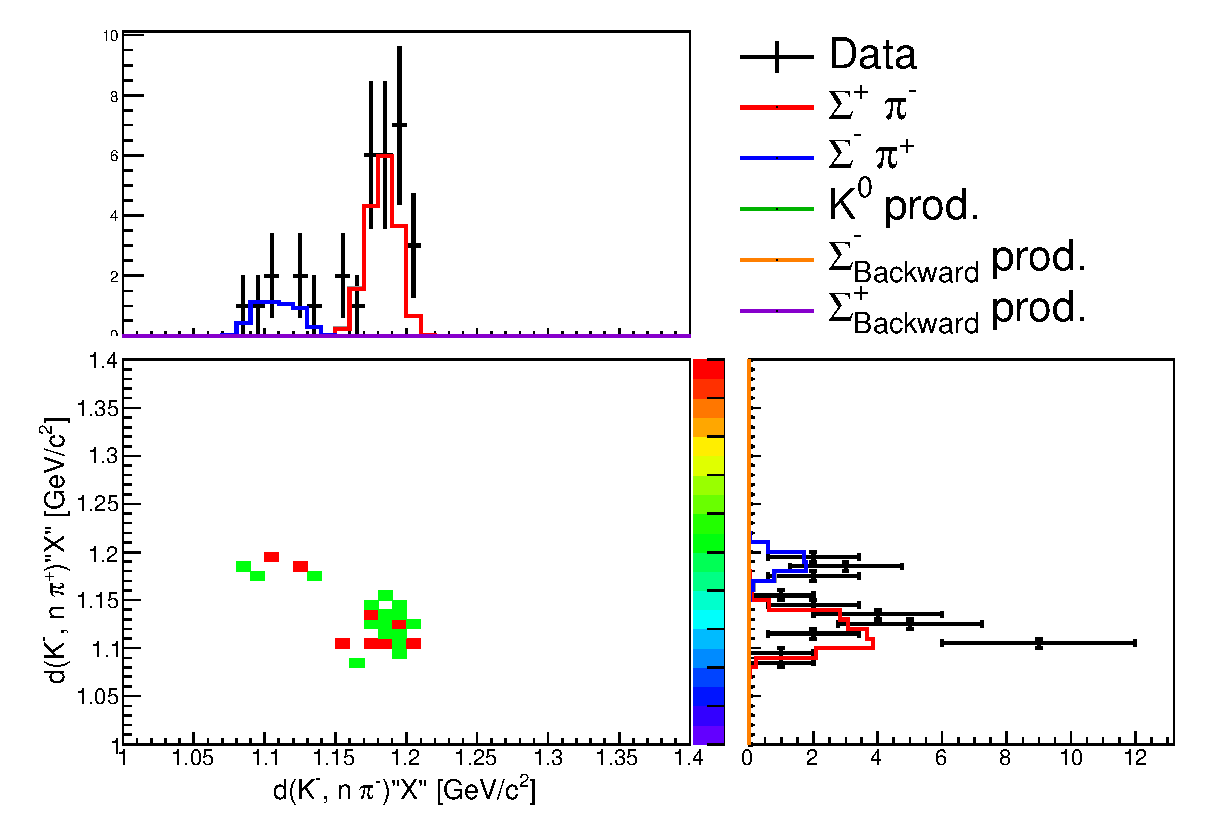
\includegraphics[width=2.2cm]{../pic/Run78/KN_ana_NC170_2sigma/KNpi_MM_1.eps}
    \end{minipage}
    \begin{minipage}{0.2\hsize}
      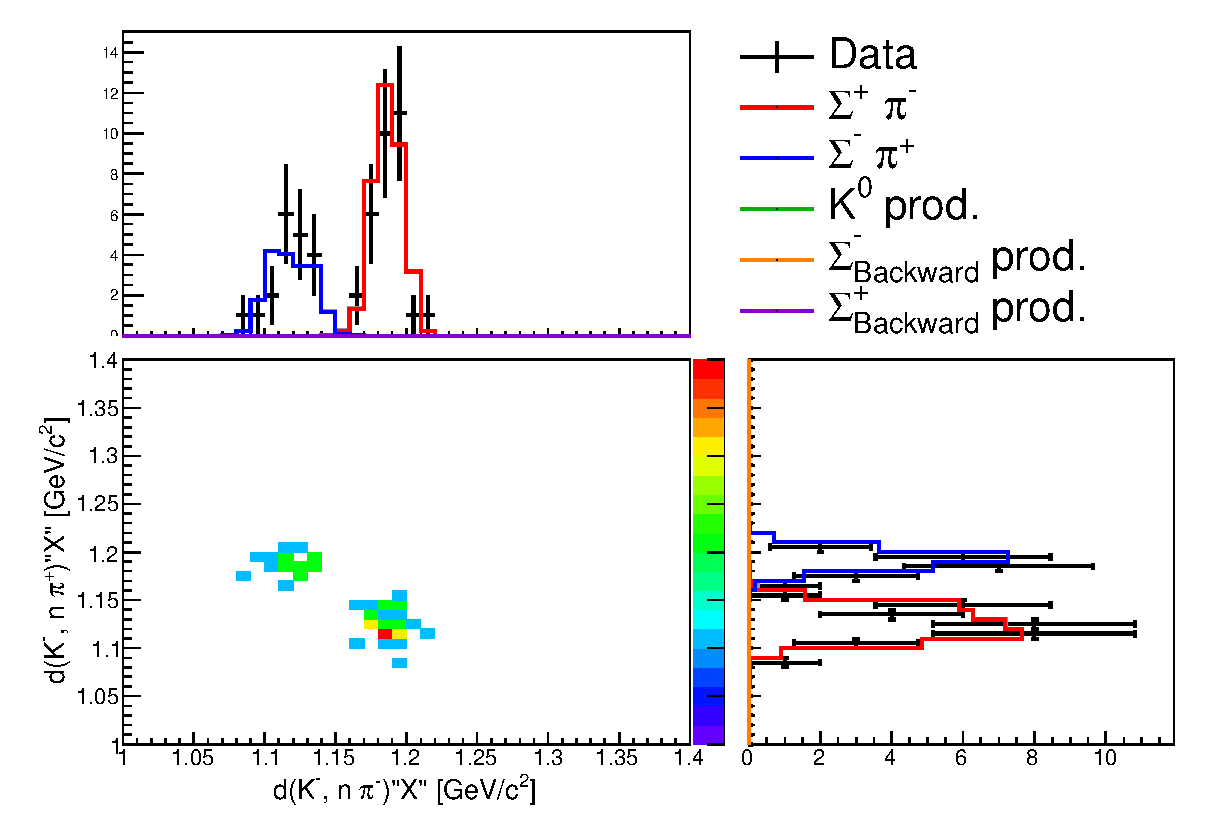
\includegraphics[width=2.2cm]{../pic/Run78/KN_ana_NC170_2sigma/KNpi_MM_2.eps}
    \end{minipage}
    \begin{minipage}{0.2\hsize}
      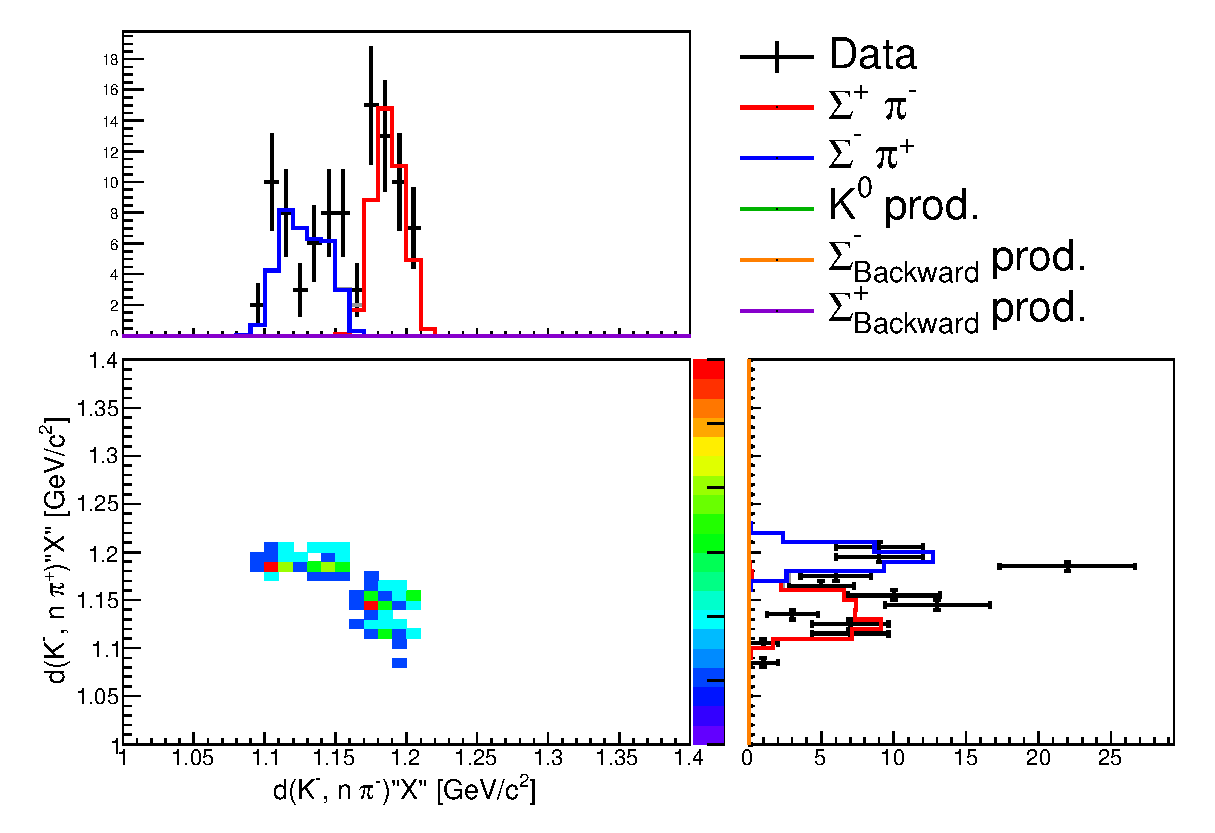
\includegraphics[width=2.2cm]{../pic/Run78/KN_ana_NC170_2sigma/KNpi_MM_3.eps}
    \end{minipage}
    \begin{minipage}{0.2\hsize}
      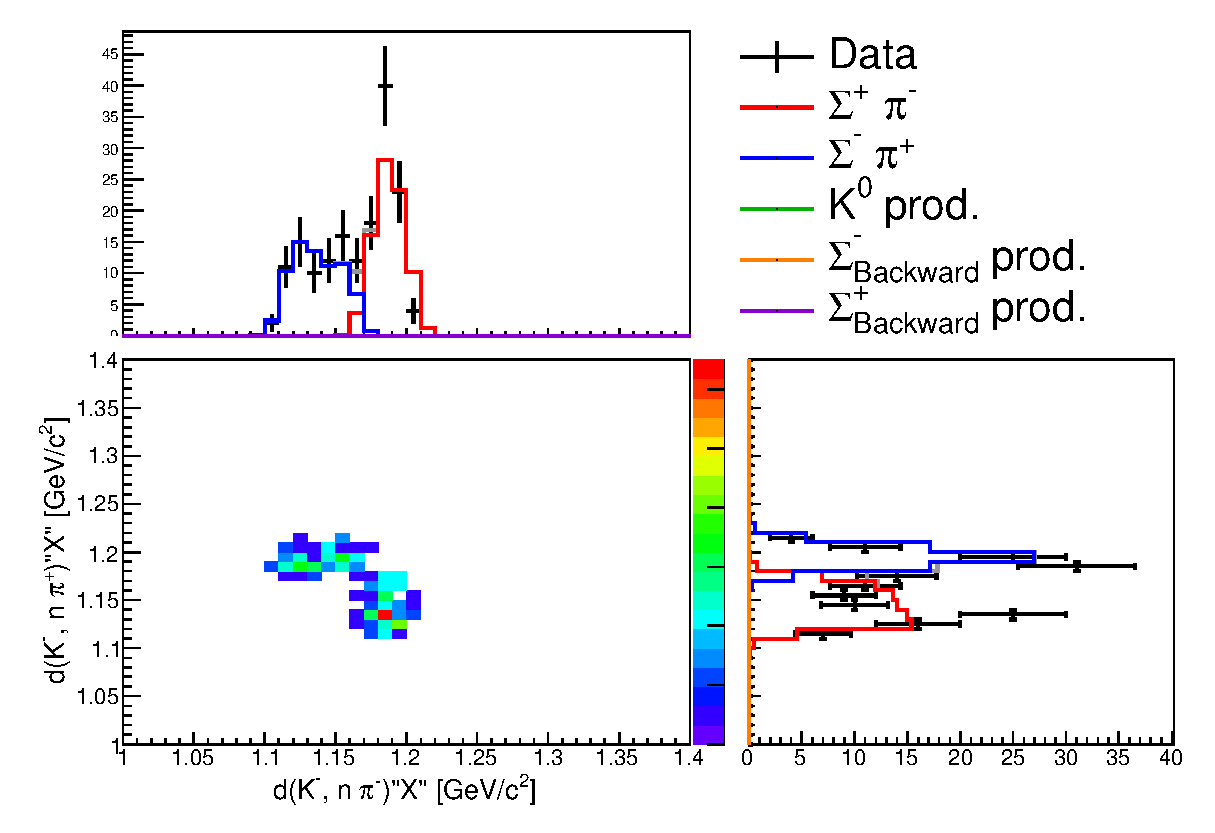
\includegraphics[width=2.2cm]{../pic/Run78/KN_ana_NC170_2sigma/KNpi_MM_4.eps}
    \end{minipage}
  \end{tabular}
  \begin{tabular}{ccccc}
    \begin{minipage}{0.2\hsize}
      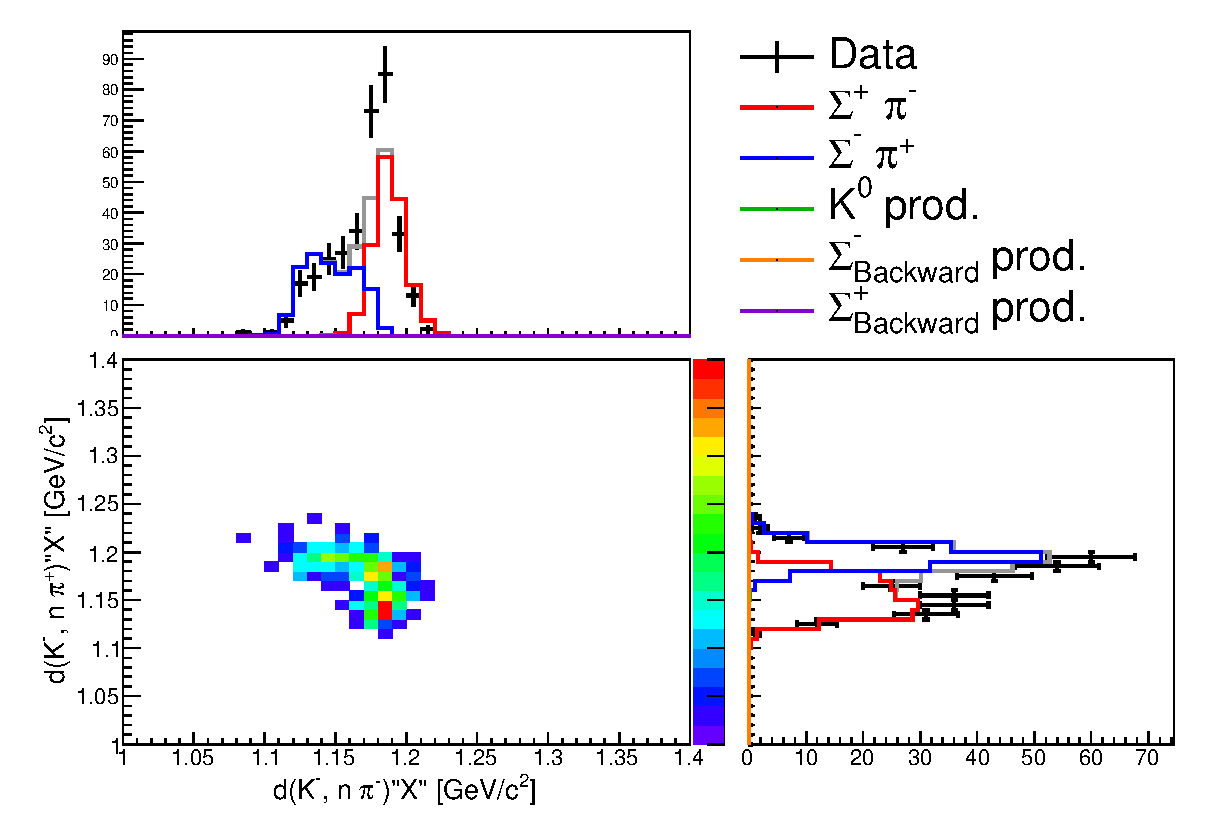
\includegraphics[width=2.2cm]{../pic/Run78/KN_ana_NC170_2sigma/KNpi_MM_5.eps}
    \end{minipage}
    \begin{minipage}{0.2\hsize}
      \includegraphics[width=2.2cm]{../pic/Run78/KN_ana_NC170_2sigma/KNpi_MM_6.eps}
    \end{minipage}
    \begin{minipage}{0.2\hsize}
      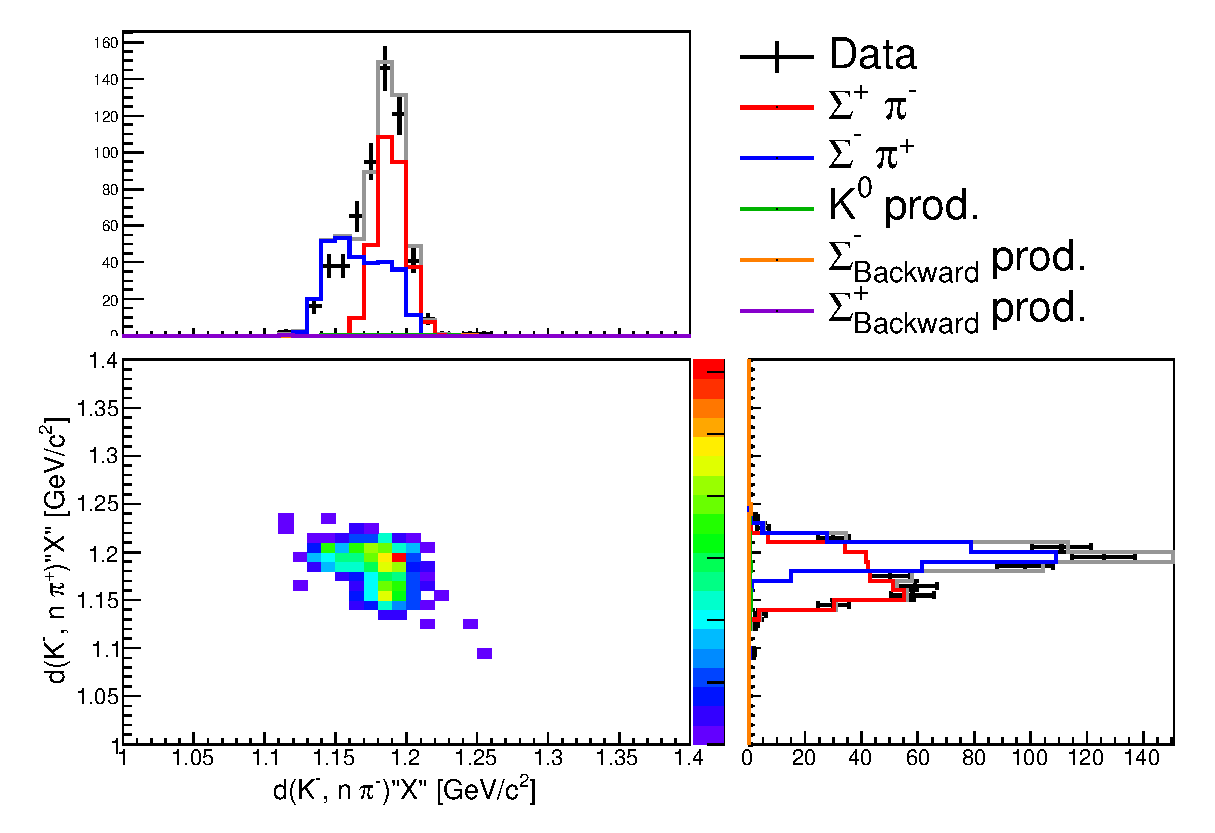
\includegraphics[width=2.2cm]{../pic/Run78/KN_ana_NC170_2sigma/KNpi_MM_7.eps}
    \end{minipage}
    \begin{minipage}{0.2\hsize}
      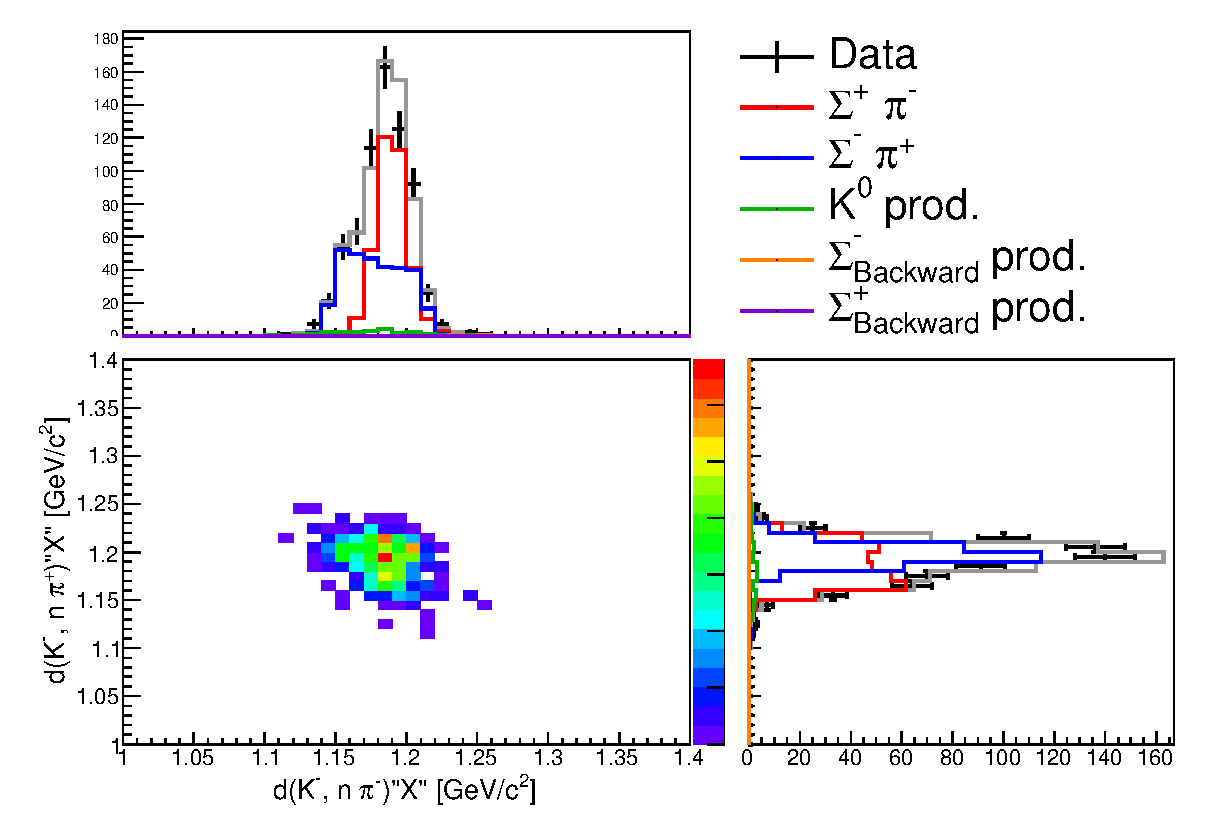
\includegraphics[width=2.2cm]{../pic/Run78/KN_ana_NC170_2sigma/KNpi_MM_8.eps}
    \end{minipage}
    \begin{minipage}{0.2\hsize}
      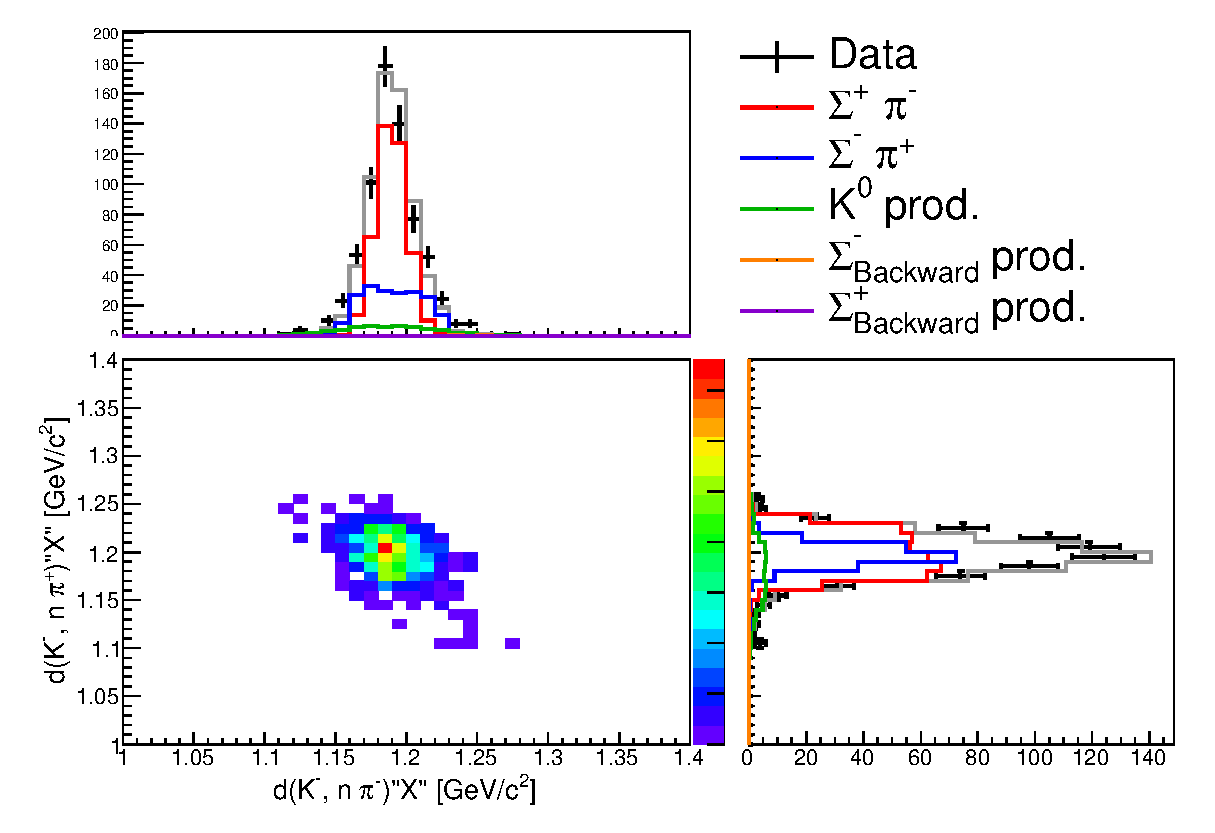
\includegraphics[width=2.2cm]{../pic/Run78/KN_ana_NC170_2sigma/KNpi_MM_9.eps}
    \end{minipage}
  \end{tabular}
  \begin{tabular}{ccccc}
    \begin{minipage}{0.2\hsize}
      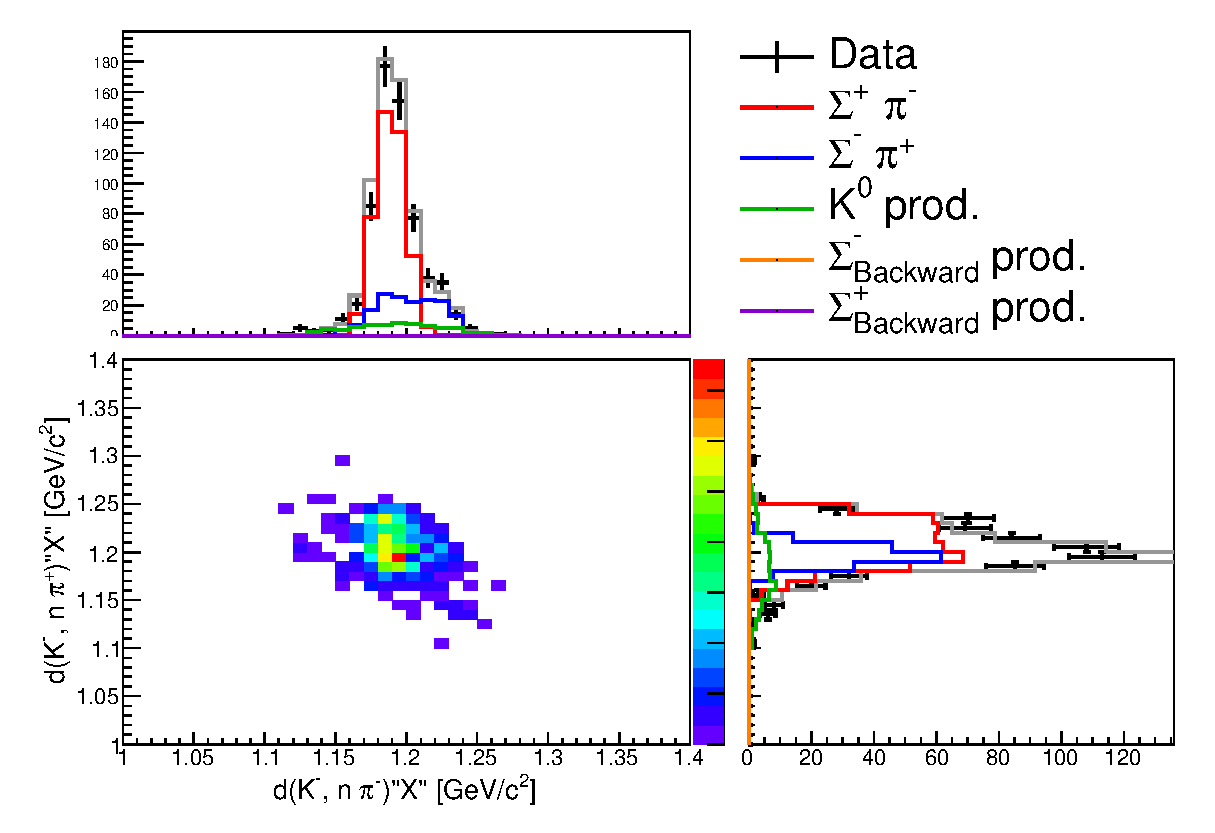
\includegraphics[width=2.2cm]{../pic/Run78/KN_ana_NC170_2sigma/KNpi_MM_10.eps}
    \end{minipage}
    \begin{minipage}{0.2\hsize}
      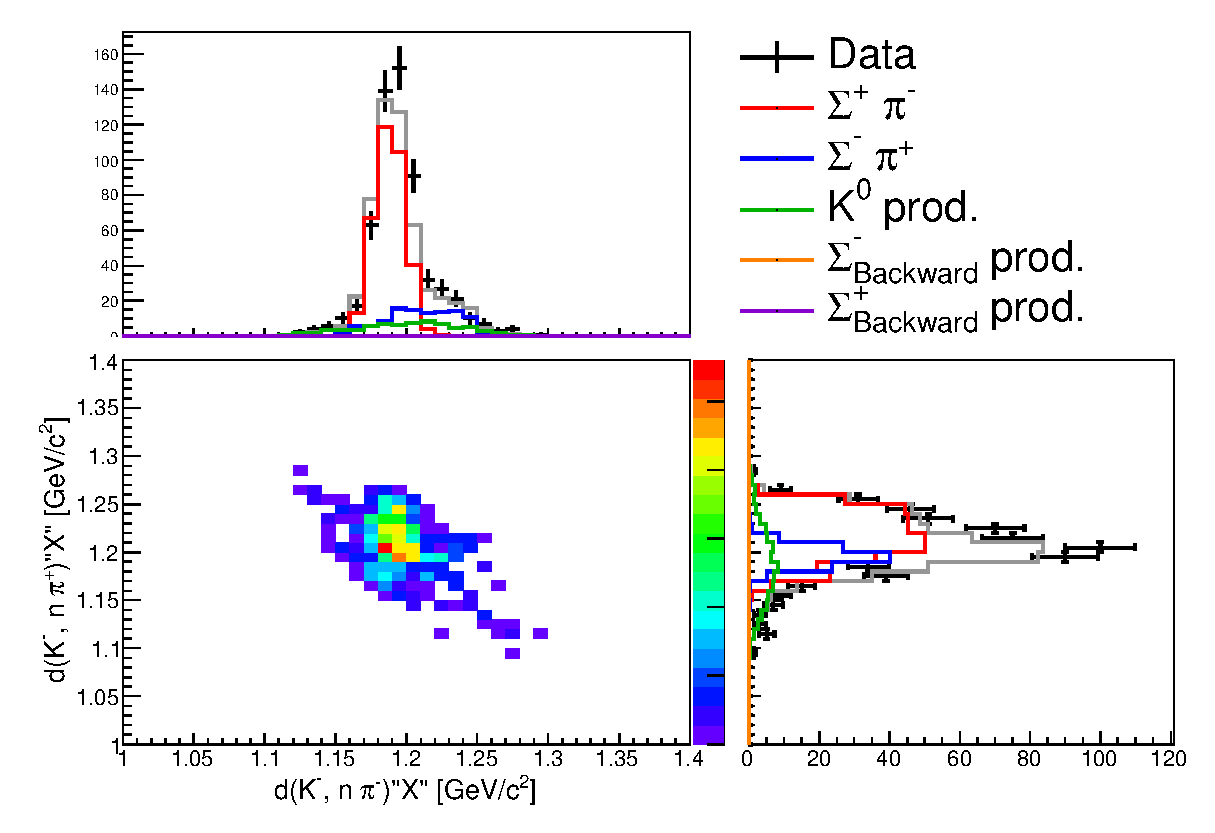
\includegraphics[width=2.2cm]{../pic/Run78/KN_ana_NC170_2sigma/KNpi_MM_11.eps}
    \end{minipage}
    \begin{minipage}{0.2\hsize}
      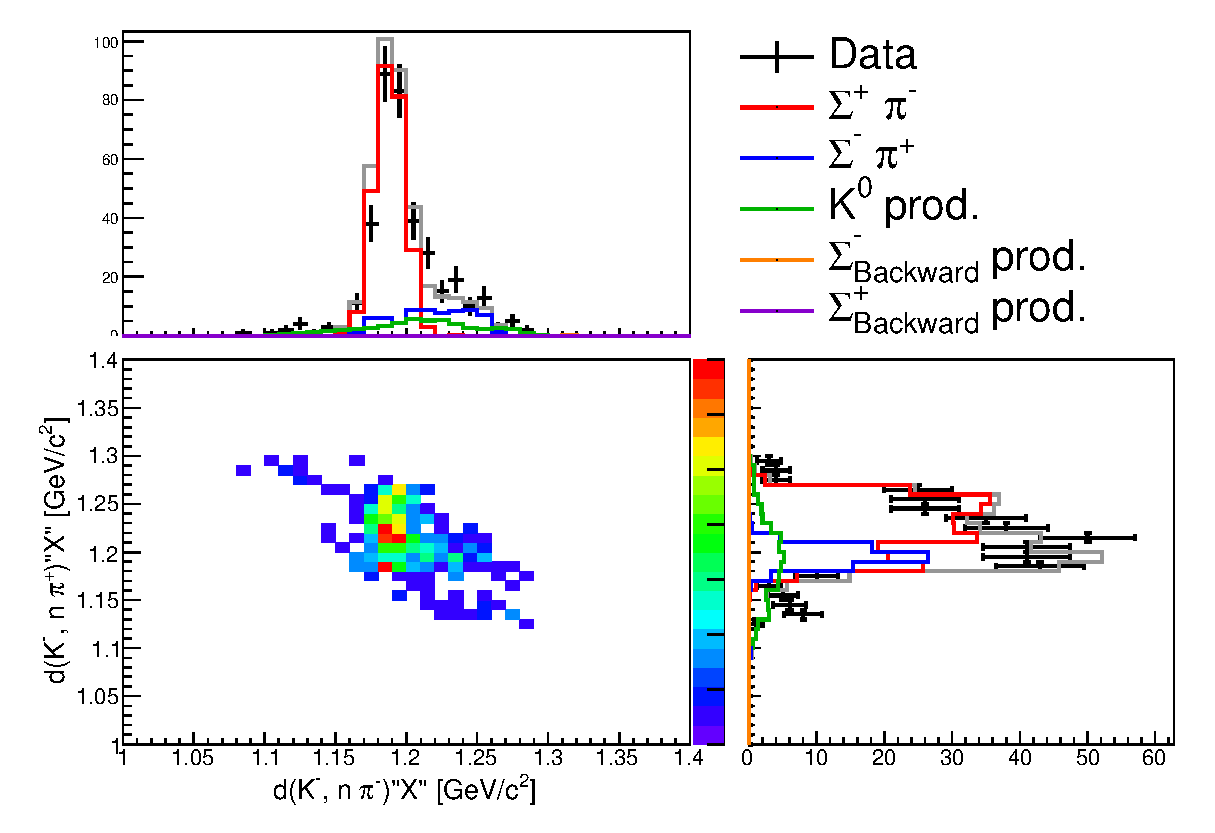
\includegraphics[width=2.2cm]{../pic/Run78/KN_ana_NC170_2sigma/KNpi_MM_12.eps}
    \end{minipage}
    \begin{minipage}{0.2\hsize}
      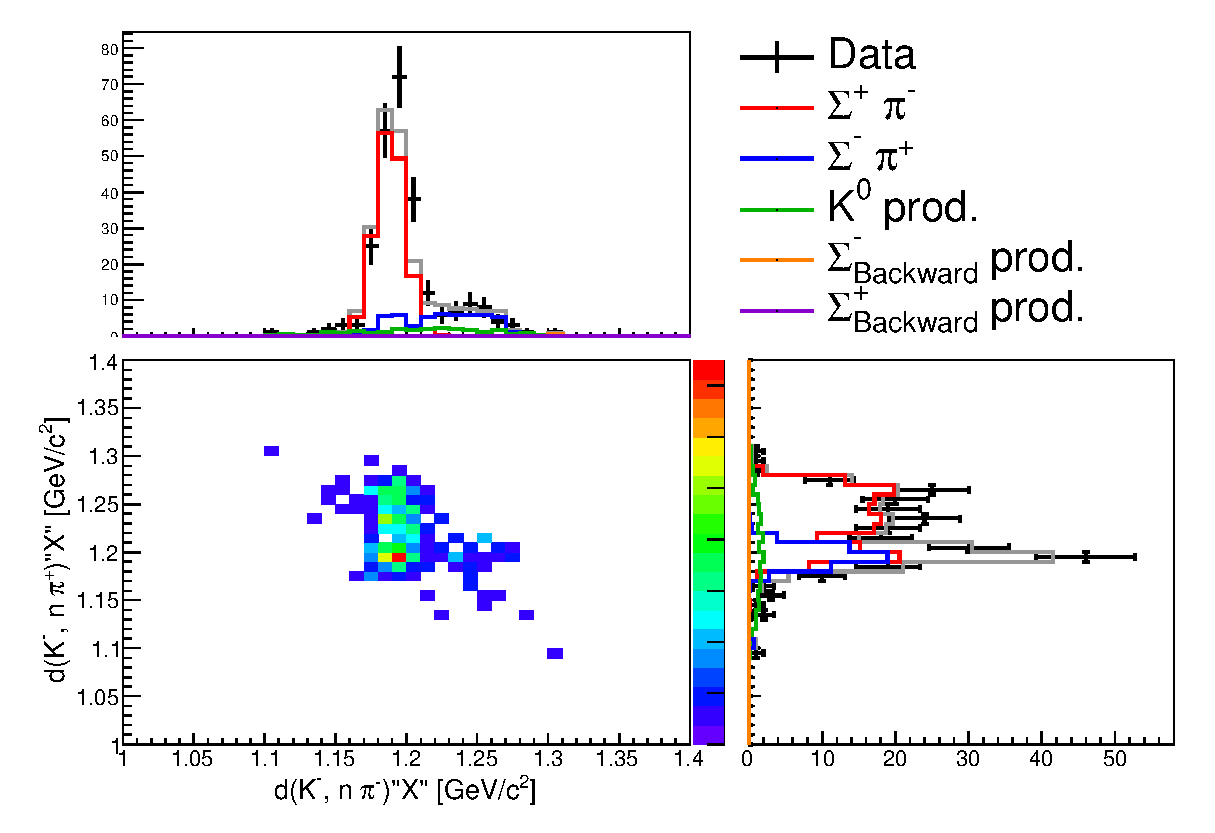
\includegraphics[width=2.2cm]{../pic/Run78/KN_ana_NC170_2sigma/KNpi_MM_13.eps}
    \end{minipage}
    \begin{minipage}{0.2\hsize}
      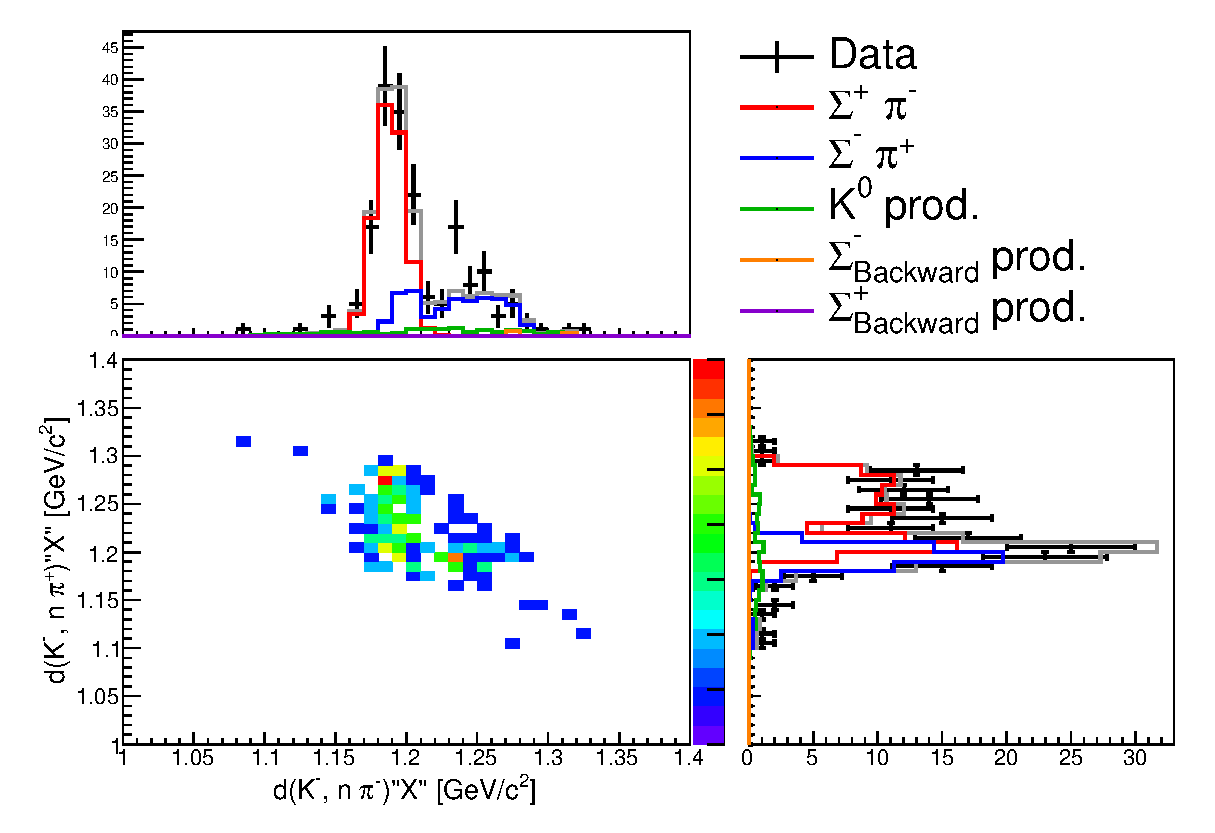
\includegraphics[width=2.2cm]{../pic/Run78/KN_ana_NC170_2sigma/KNpi_MM_14.eps}
    \end{minipage}
  \end{tabular}
  \begin{tabular}{ccccc}
    \begin{minipage}{0.2\hsize}
      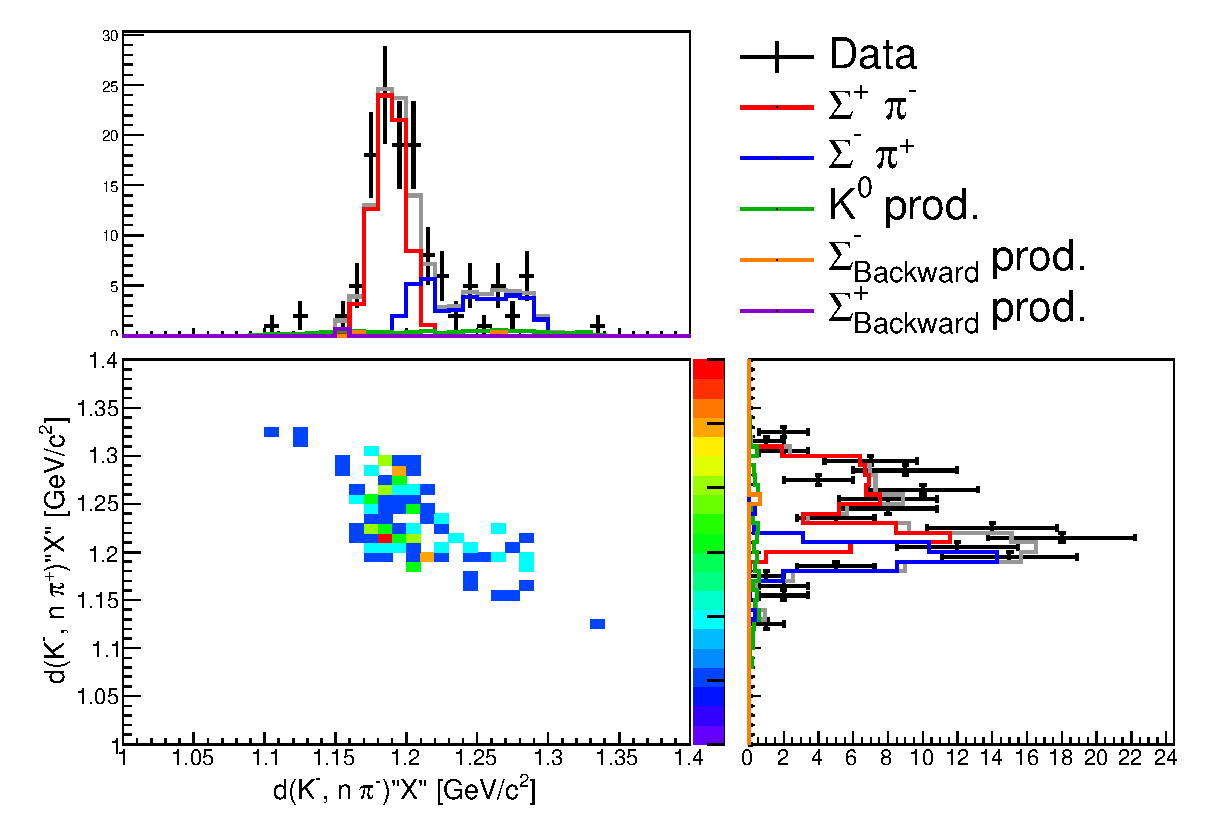
\includegraphics[width=2.2cm]{../pic/Run78/KN_ana_NC170_2sigma/KNpi_MM_15.eps}
    \end{minipage}
    \begin{minipage}{0.2\hsize}
      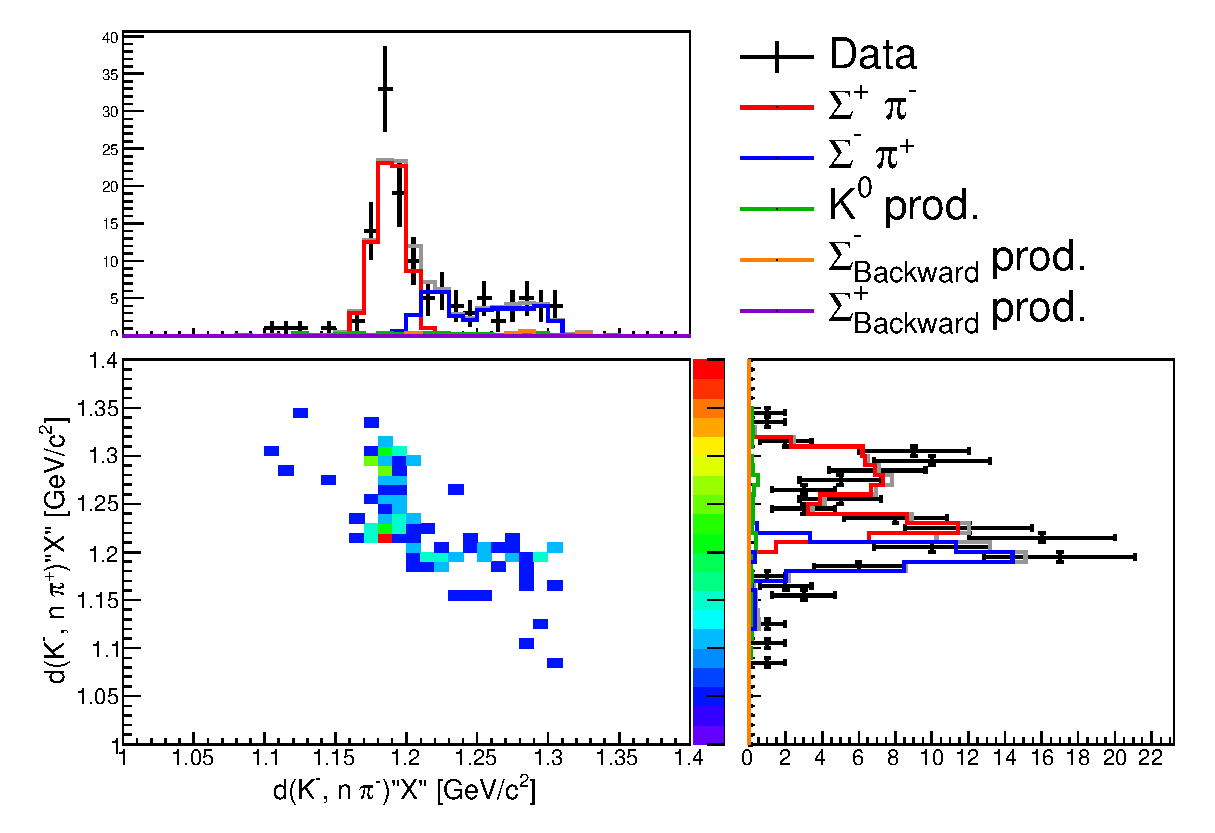
\includegraphics[width=2.2cm]{../pic/Run78/KN_ana_NC170_2sigma/KNpi_MM_16.eps}
    \end{minipage}
    \begin{minipage}{0.2\hsize}
      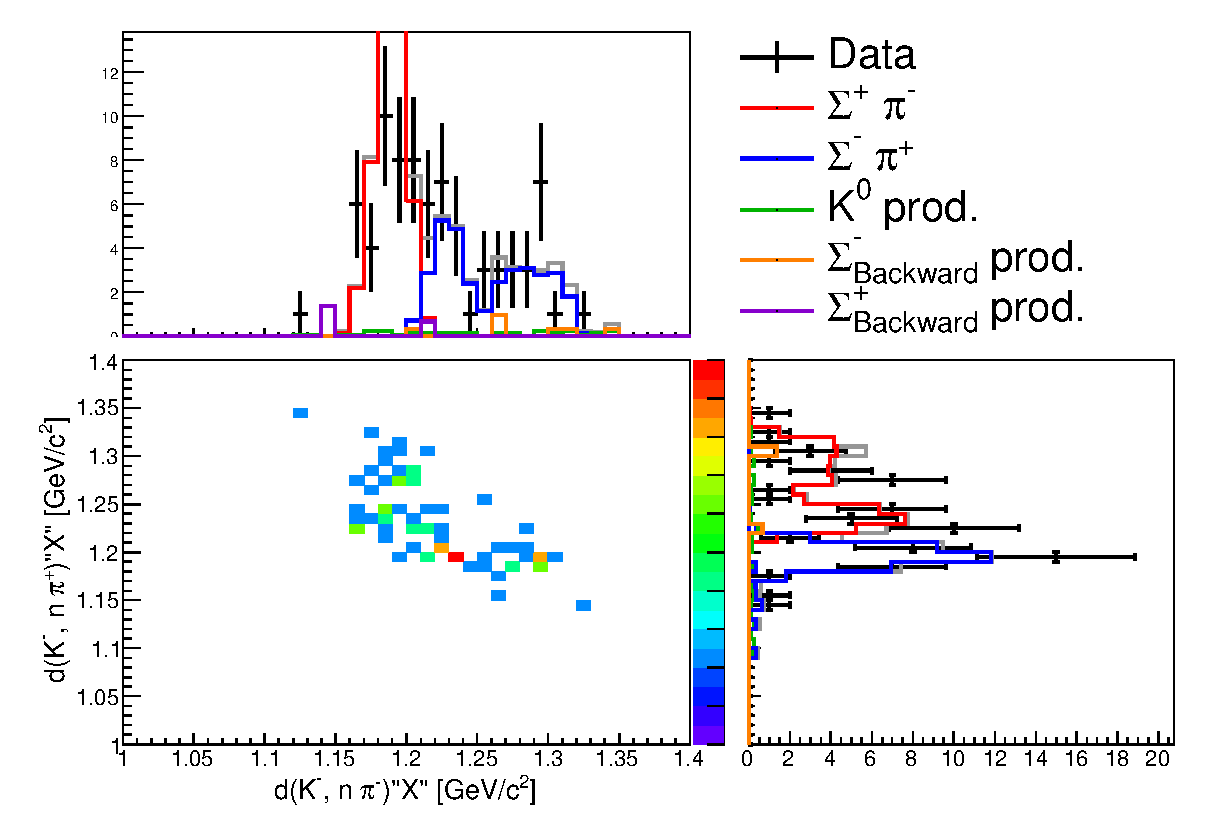
\includegraphics[width=2.2cm]{../pic/Run78/KN_ana_NC170_2sigma/KNpi_MM_17.eps}
    \end{minipage}
    \begin{minipage}{0.2\hsize}
      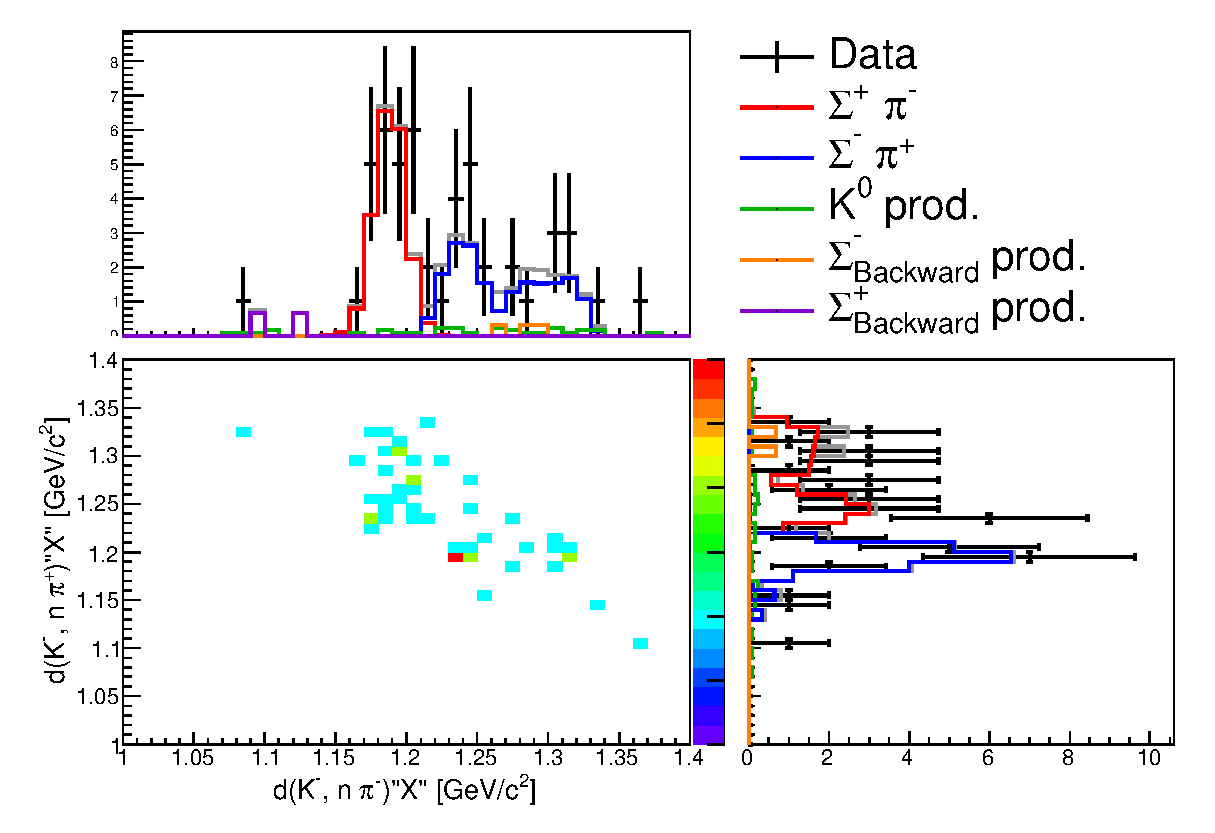
\includegraphics[width=2.2cm]{../pic/Run78/KN_ana_NC170_2sigma/KNpi_MM_18.eps}
    \end{minipage}
    \begin{minipage}{0.2\hsize}
      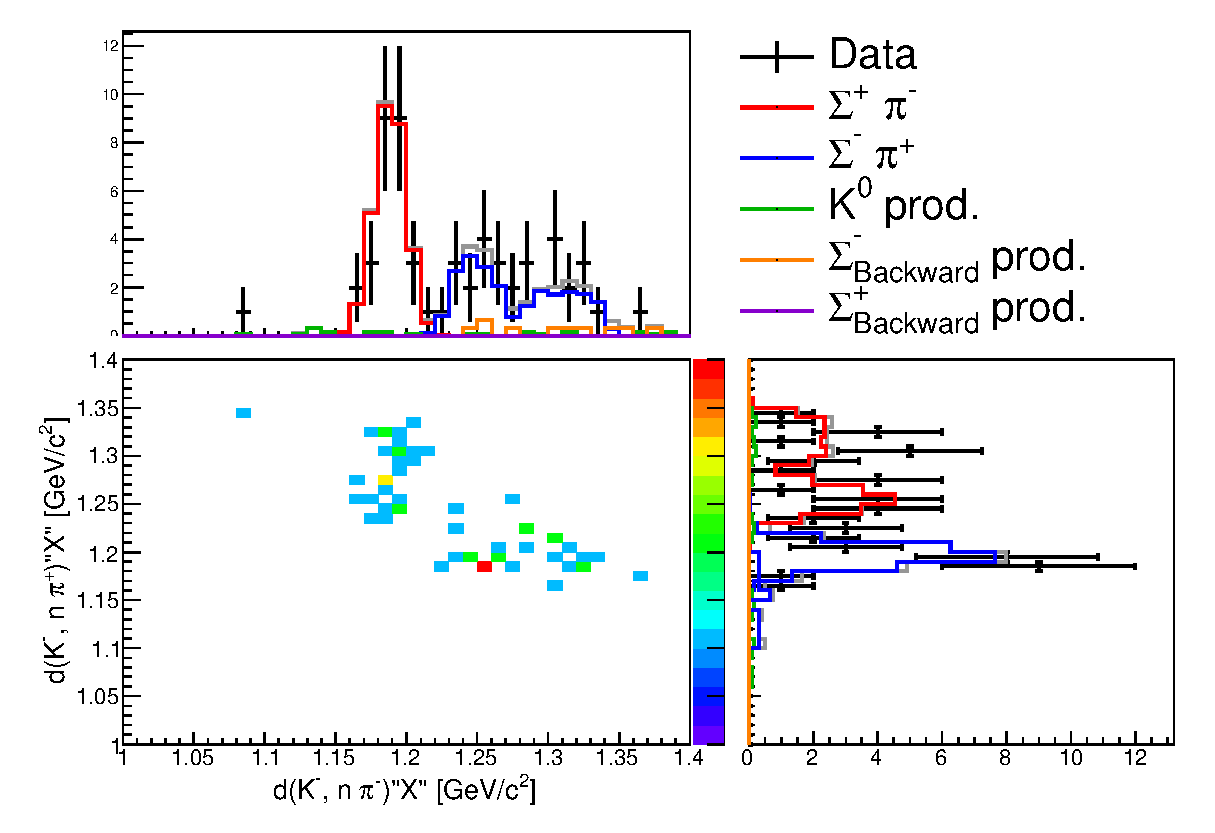
\includegraphics[width=2.2cm]{../pic/Run78/KN_ana_NC170_2sigma/KNpi_MM_19.eps}
    \end{minipage}
  \end{tabular}
  \begin{tabular}{ccccc}
    \begin{minipage}{0.2\hsize}
      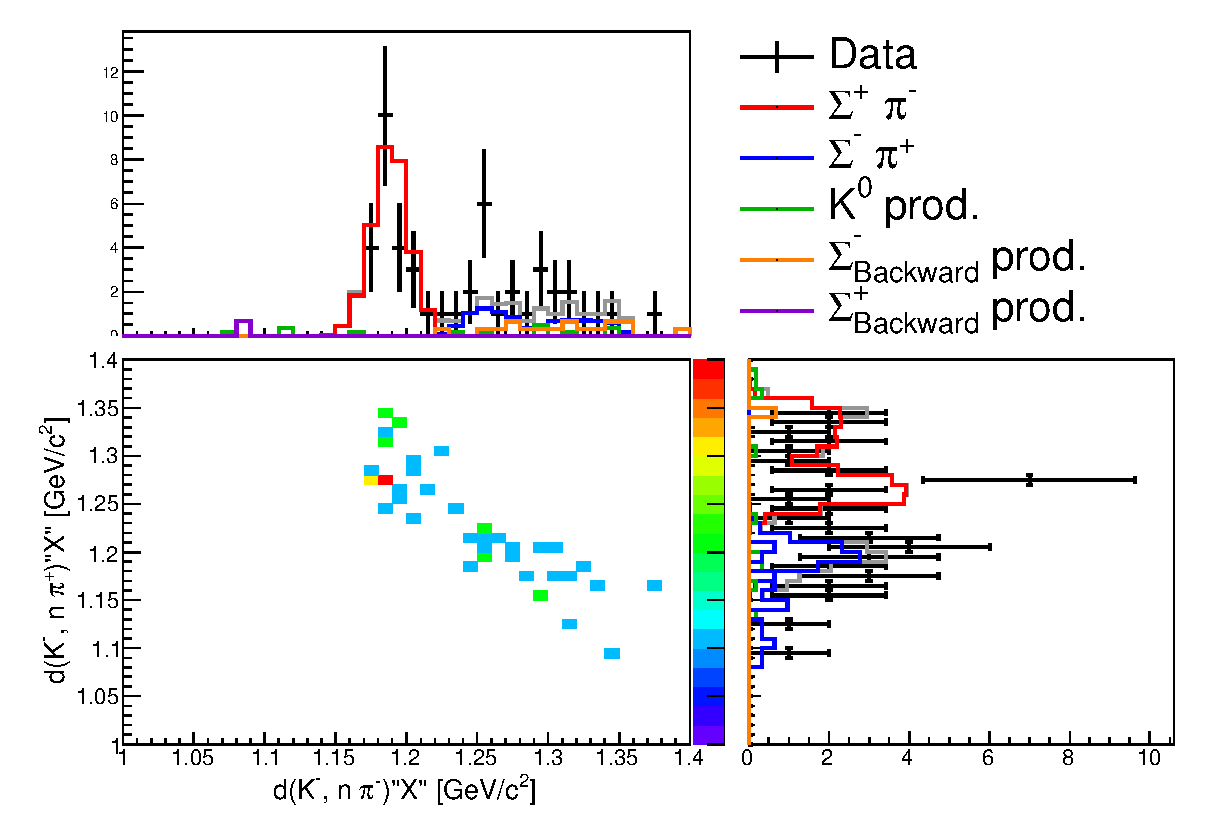
\includegraphics[width=2.2cm]{../pic/Run78/KN_ana_NC170_2sigma/KNpi_MM_20.eps}
    \end{minipage}
    \begin{minipage}{0.2\hsize}
      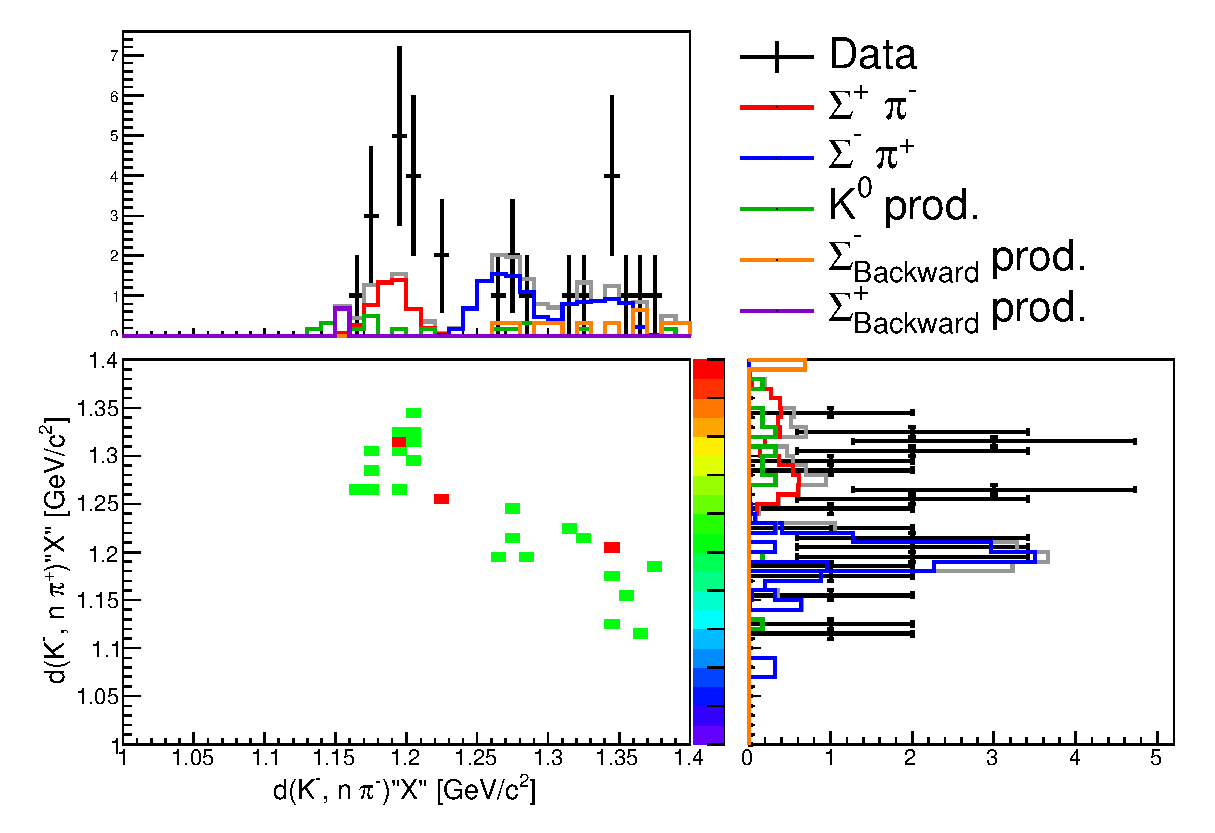
\includegraphics[width=2.2cm]{../pic/Run78/KN_ana_NC170_2sigma/KNpi_MM_21.eps}
    \end{minipage}
    \begin{minipage}{0.2\hsize}
      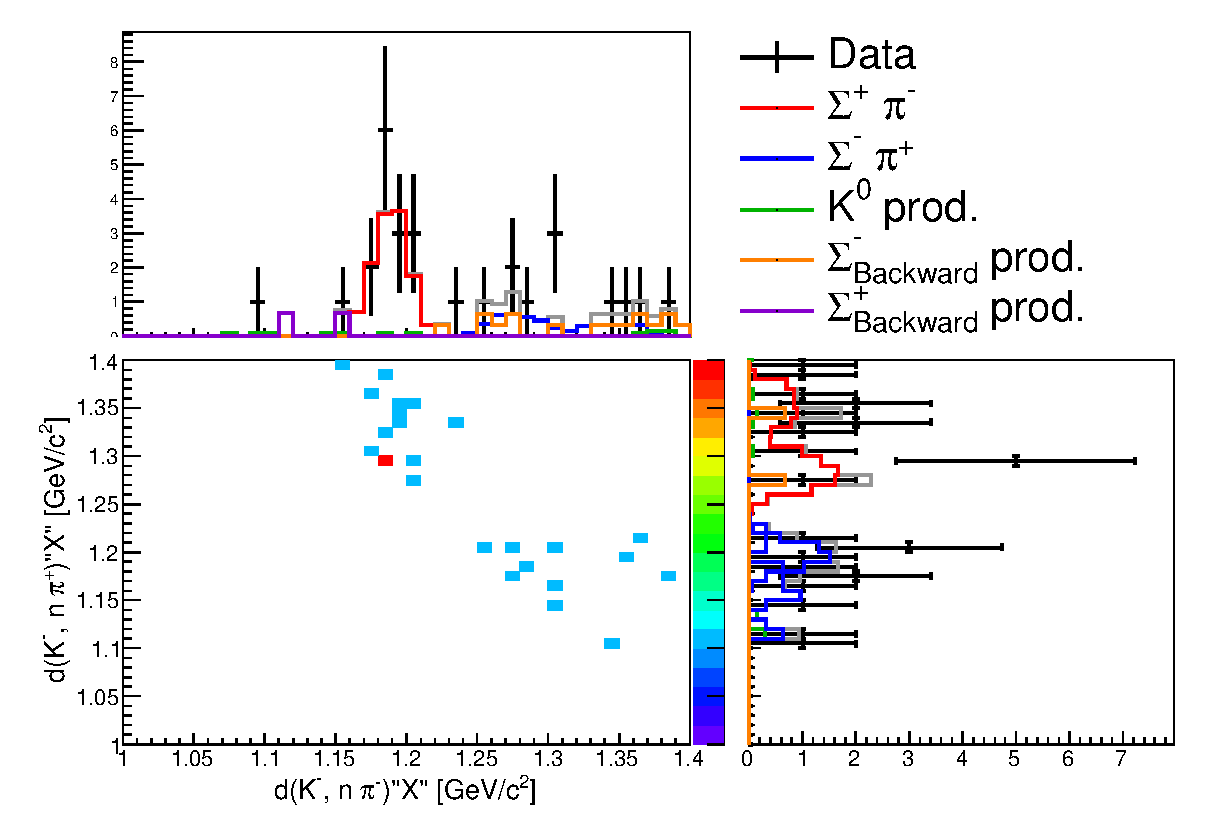
\includegraphics[width=2.2cm]{../pic/Run78/KN_ana_NC170_2sigma/KNpi_MM_22.eps}
    \end{minipage}
    \begin{minipage}{0.2\hsize}
      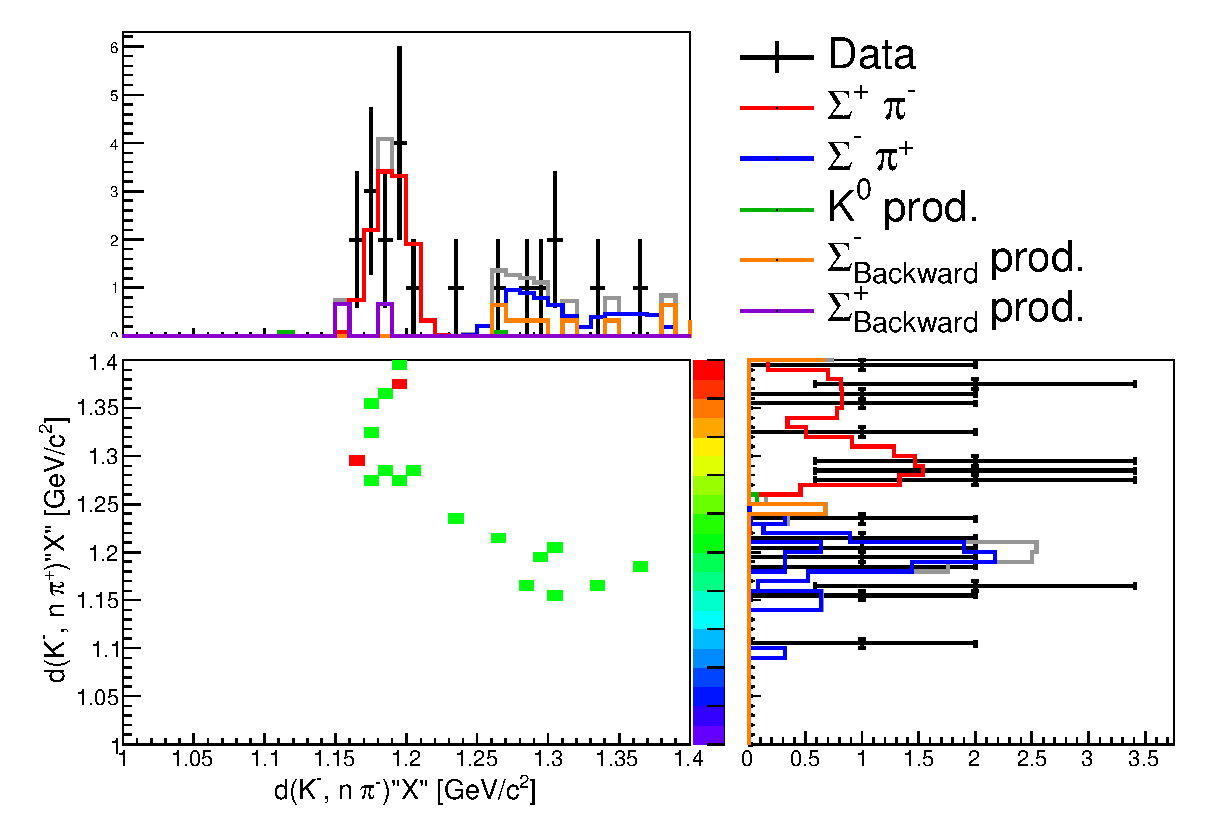
\includegraphics[width=2.2cm]{../pic/Run78/KN_ana_NC170_2sigma/KNpi_MM_23.eps}
    \end{minipage}
    \begin{minipage}{0.2\hsize}
      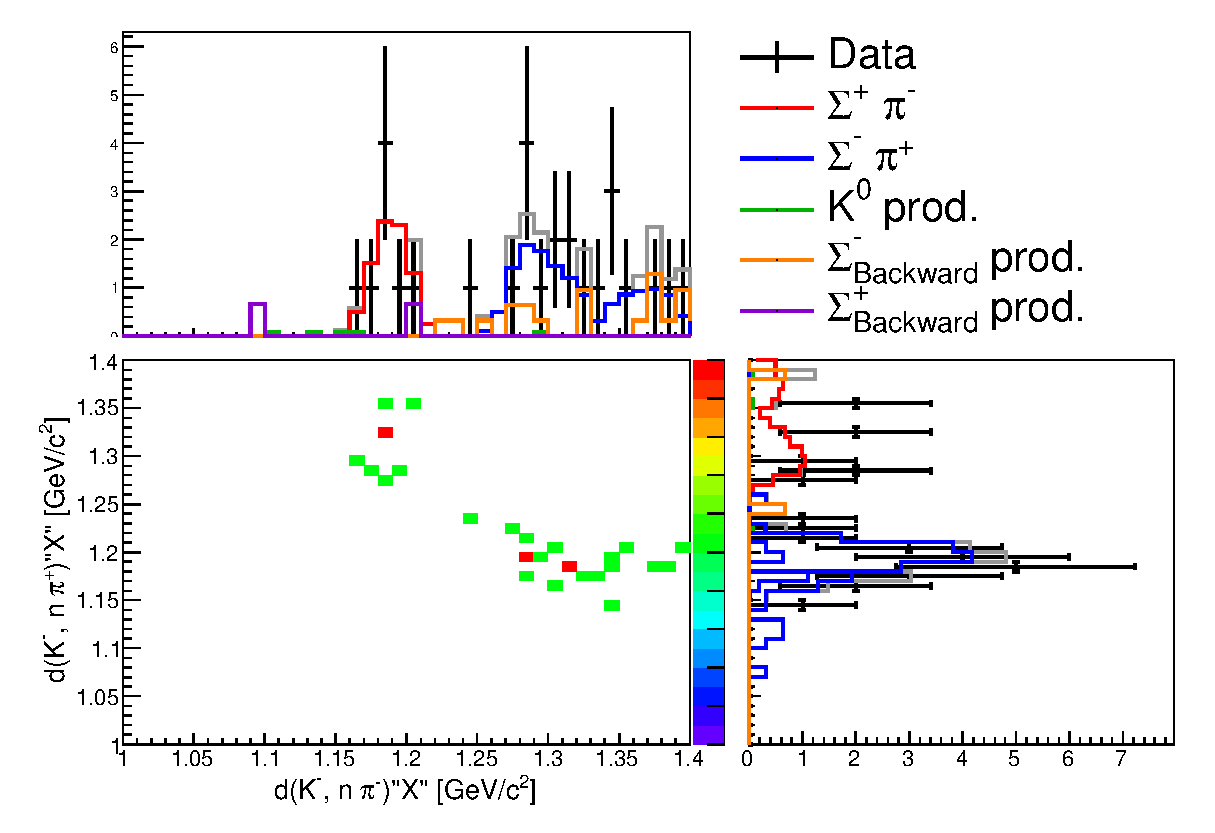
\includegraphics[width=2.2cm]{../pic/Run78/KN_ana_NC170_2sigma/KNpi_MM_24.eps}
    \end{minipage}
  \end{tabular}
  \label{fig:fit_KNpi_MM}
  \caption{
    These figures are presented separately for each bin of $d(K^-, n)$ for fitting to separate $\pi^- \Sigma^+$ and $\pi^+ \Sigma^-$ modes.
    The top left figure shows the lowest missing mass in the $1.35$-$1.36$GeV bin, with the next bin represented as one goes to the right.
    In other words, one row is shown for the 0.05GeV region.
  }
\end{figure}

\begin{figure}[htbp]
  \centering

  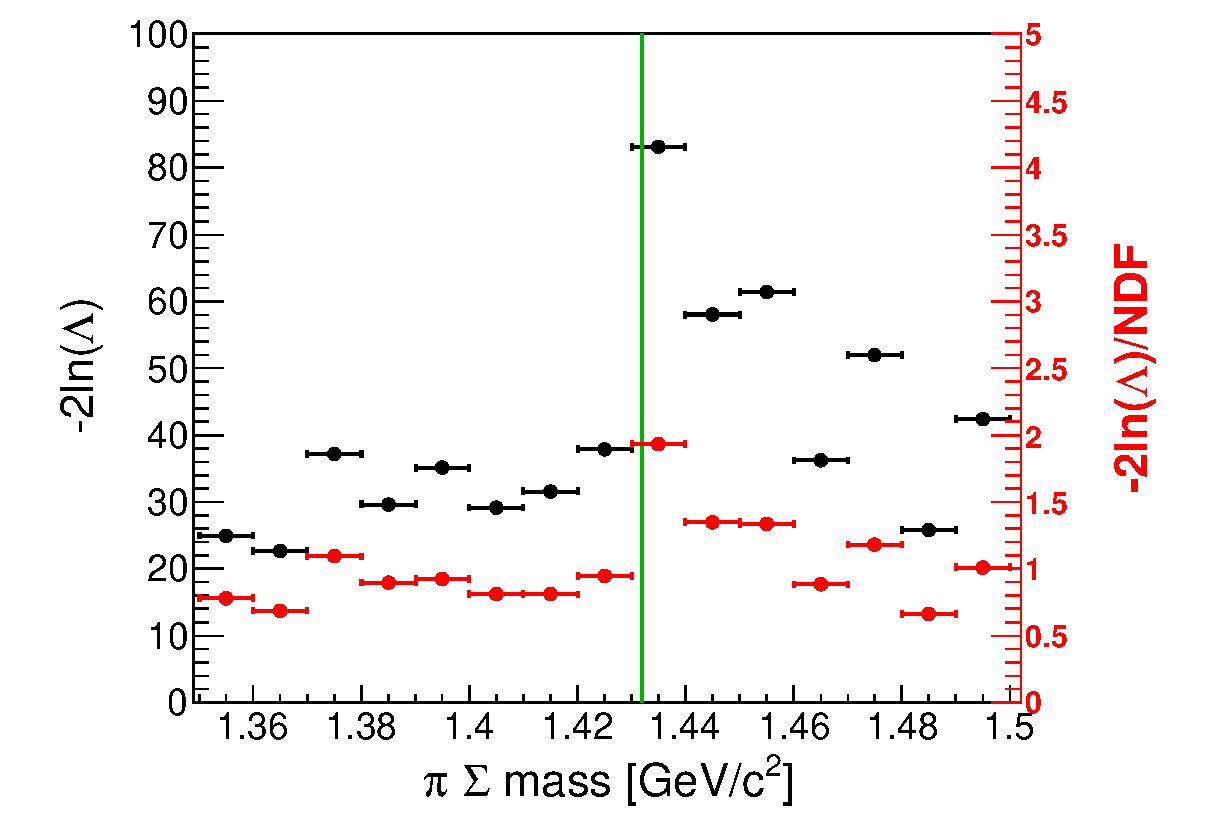
\includegraphics[width=8cm]{../pic/Dron/tempFit_KNpi_MM_Chi2.eps}
  \caption{
    This figure shows the template fitting $-2\log\Lambda$ and $-2\log\Lambda/NDF$ for the separation of $\pi^- \Sigma^+$ and $\pi^+ \Sigma^-$ modes in each $d(K^-, n)$ bin.
    Black and red indicate $-2\log\Lambda$ and $-2\log\Lambda/NDF$, respectively.
    The horizontal axis is represented for $d(K^-, n)$ bins.
  }
  \label{fig:tempFit_KNpi_Chi2}
\end{figure}


The fitting to separate the $\pi^-\Sigma^+$ and $\pi^+\Sigma^-$ modes is performed for events from $K^-- d \rightarrow n \pi^+ \pi- n$, excluding $K^0 $and $\Sigma^{\pm}_{forward}$ production.
However, the background leakage is estimated by scaling the distribution reconstructed in the MC simulation by the intensity estimated by the invariant mass fitting.
This fitting is performed each bin of the missing mass of $d(K^-, n)$, since the scattering amplitude of $\bar{K}N \rightarrow \pi \Sigma$ depends on the $\pi \Sigma$ invariant mass.
For this fitting we use the $d(K^-, n \pi^-)$ and $d(K^-, n \pi^+)$ missing masses as shown in Fig.\ref{fig:fit_KNpi_MM_all}.
This figure shows the sum of the $d(K^- , n)$ bins.
The bottom left figure shows a two-dimensional figure of the $d(K^-, n \pi^-)$ and $d(K^-, n \pi^+)$ missing masses on the horizontal and vertical axes, respectively.
The top and right figures show the projections of the respective axes.
The missing mass of $d(K^-, n \pi)$ makes a peak at $\Sigma$ for the correct combination for the missing $\Sigma$, but is widely distributed in the kinematic region for the opposite charge.
For example, for $d(K^-, n \pi^-)$, the $\pi^- \Sigma^+$ mode has a peak structure as shown by the red line,
whereas the $\pi^+ \Sigma^-$ mode has a widely distributed structure as shown by the blue line.

Fig.\ref{fig:fit_KNpi_MM} shows the results for the fitting of each bin of $d(K^-, n)$ separately.
Fig.\ref{fig:tempFit_KNpi_Chi2} shows the $-2\log\Lambda$ and $-2\log\Lambda/NDF$ of this fitting in each $d(K^-, n)$ bin in black and red, respectively.

Fitting to estimate background and to separate $\pi^- \Sigma^+$ and $\pi^+ \Sigma^-$ modes cannot be performed simultaneously as they use different event samples.
They are therefore repeated in the following steps.

First, the separation of $\pi^- \Sigma^+$ and $\pi^+ \Sigma^-$ modes is performed without considering the background.
The obtained distribution of backward $\pi^{\mp} \Sigma^{\pm}$ modes is used for fitting to estimate the background,
which is then fed back into the fitting of the separation of $\pi^- \Sigma^+$ and $\pi^+ \Sigma^-$ modes.
After five iterations of this procedure, fitting is performed considering 2-step and direct $\Lambda(1520)$ generation for $K^0$ generation, which is described in the Appendix.\ref{apendix:K0_event}.
Finally, fitting of the separation of the $\pi^- \Sigma^+$ and $\pi^+ \Sigma^-$ modes is performed to obtain the final $\pi \Sigma$ spectrum as shown in Fig.\ref{fig:piS_num}..

\begin{figure}[htbp]
  \centering
  
  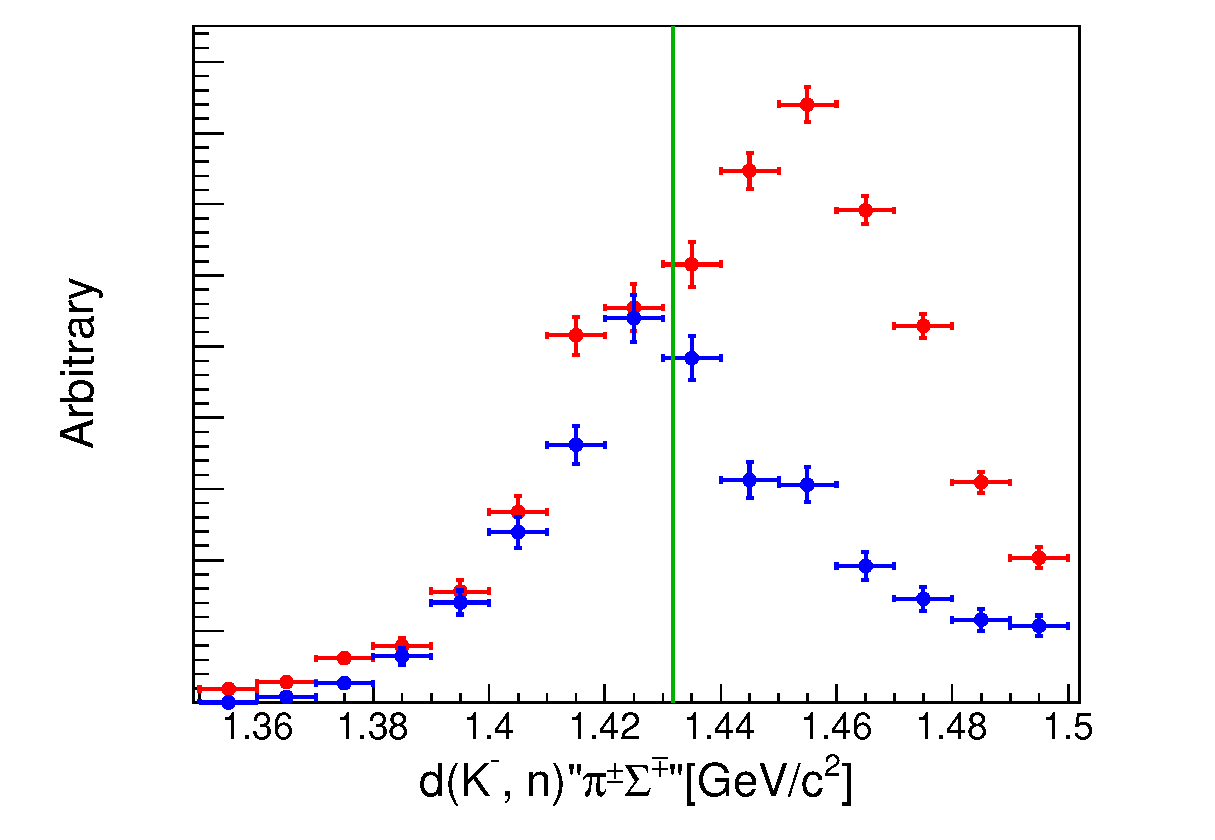
\includegraphics[width=8cm]{../pic/Dron/piS_num.eps}
  \caption{
    The $\pi^-\Sigma^+$ and $\pi^+\Sigma^-$ mode spectra obtained by template fitting are shown in arbitrary units.
    Red and blue lines indicate $\pi^-\Sigma^+$ and $\pi^+\Sigma^-$, respectively.
    The green vertical line is indicated the $\bar{K}N$ threshold.        
  }
  \label{fig:piS_num}
\end{figure}



%% \begin{frame}{Template fitting to decompose $K^0$ production}
  \begin{figure}
    \centering
    Invariant mass of $n K^0$\\
    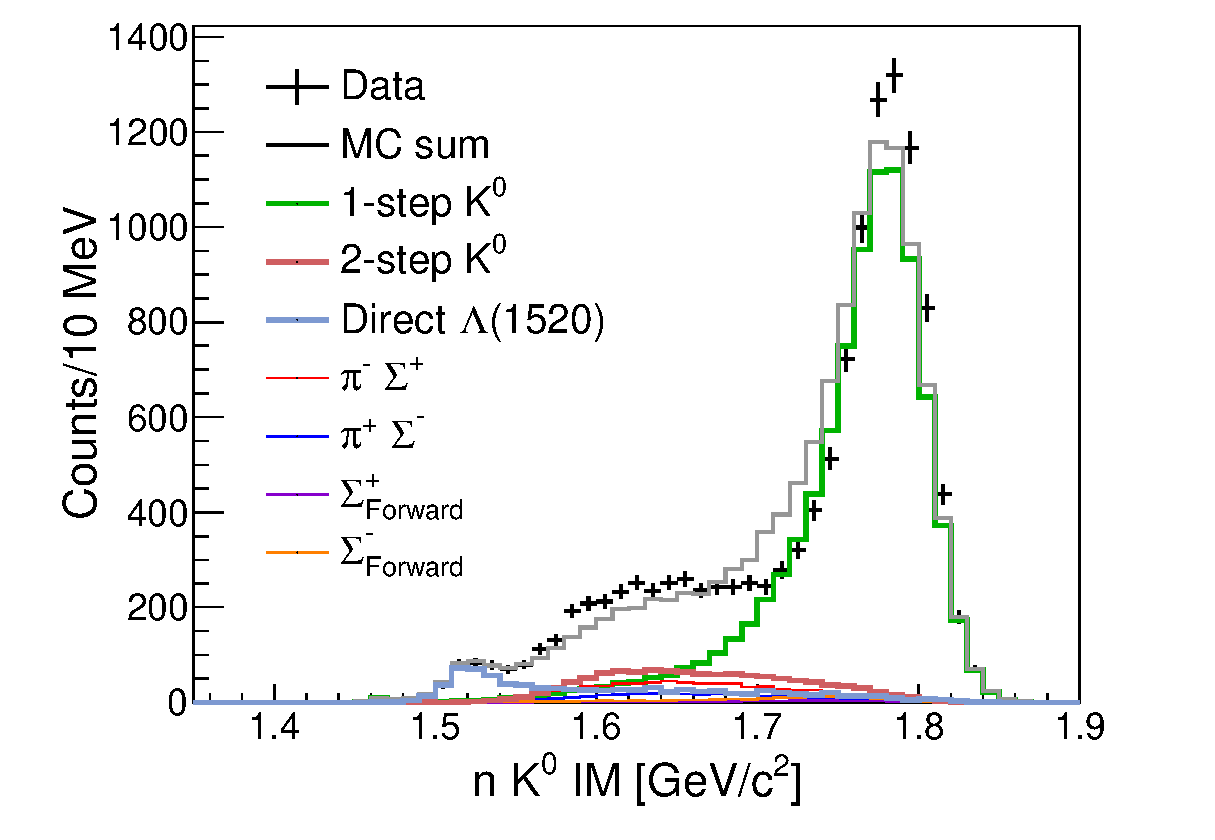
\includegraphics[width=7.5cm]{../pic/Dron/K0_ana/npipi_IM_K0.eps}
  \end{figure}
  \centering
  2-step like component is seen about 11.5\%.\\
  Direct-$\Lambda(1520)$ prod. is seen about 7.7\%.\\
\end{frame}



\newcommand{\IMfitChiSquare}{1077.4}
\newcommand{\IMfitNDF}{352}
\newcommand{\IMfitChiNDF}{3.06}

\newcommand{\KzeroFitChi}{275.2}
\newcommand{\KzeroFitNDF}{43}
\newcommand{\KzeroFitChiNDF}{6.40}

\newcommand{\KzeroOneStepRatio}{80.9 \pm 1.3\%}
\newcommand{\KzeroTwoStepRatio}{11.5 \pm 1.0\%}
\newcommand{\KzeroLsRatio}{7.7 \pm 0.6\%}

\newcommand{\fitScatLength}{-1.05 \pm 0.12 (fit.) \pm +0.09 (syst.) + [ 0.86 \pm 0.15 (fit.) ^{+0.07} _{-0.08} (syst.)]i}
\newcommand{\fitEffRange}{-0.22 \pm 0.40 (fit.) ^{+0.05} _{-0.06} (syst.) + [ -0.42 \pm 0.16 (fit.) ^{+0.12} _{-0.08} (syst.)]i}
\newcommand{\fitPole}{1418.3 ^{+7.5} _{-2.4} (fit.)^{+0.9}_{-1.1} (syst.)}
\newcommand{\fitWidth}{-27.8^{+9.5}_{-0.9} (fit.)^{+1.9}_{-2.1} (syst.)}

\newcommand{\fitAscaleIz}{0.562 \pm 0.015}
\newcommand{\fitAscaleIo}{1.070 \pm 0.040}
\newcommand{\fitAscaleIzVal}{0.562}
\newcommand{\fitAscaleIzErr}{0.015}
\newcommand{\fitAscaleIoVal}{1.070}
\newcommand{\fitAscaleIoErr}{0.040}
\newcommand{\fitAscaleChi}{691/42}
\newcommand{\fitAscaleChiNum}{16.4}

\newcommand{\fitBscaleIz}{0.721 \pm 0.016}
\newcommand{\fitBscaleIo}{1.423 \pm 0.055}
\newcommand{\fitBscaleIzVal}{0.721}
\newcommand{\fitBscaleIoVal}{1.423}
\newcommand{\fitBscaleIzErr}{0.016}
\newcommand{\fitBscaleIoErr}{0.055}
\newcommand{\fitBscaleChi}{220/42}
\newcommand{\fitBscaleChiNum}{5.25}

\newcommand{\fitBBChi}{187/41}
\newcommand{\fitBBChiNum}{4.56}
\newcommand{\fitBBIz}{0.686 \pm 0.017}
\newcommand{\fitBBIo}{1.462 \pm 0.059}
\newcommand{\fitBBphase}{0.828 \pm 0.030}
\newcommand{\fitBBIzVal}{0.686}
\newcommand{\fitBBIoVal}{1.462}
\newcommand{\fitBBphaseVal}{0.828}
\newcommand{\fitBBIzErr}{0.017}
\newcommand{\fitBBIoErr}{0.059}
\newcommand{\fitBBphaseErr}{0.030}
\newcommand{\fitBBDegree}{34.1^{+3.0}_{-3.2}}

\newcommand{\fitBChi}{184/41}
\newcommand{\fitBChiNum}{4.48}
\newcommand{\fitBIz}{0.682 \pm 0.017}
\newcommand{\fitBIo}{1.570 \pm 0.058}
\newcommand{\fitBphase}{0.811 \pm 0.030}
\newcommand{\fitBIzVal}{0.682}
\newcommand{\fitBIoVal}{1.570}
\newcommand{\fitBphaseVal}{0.811}
\newcommand{\fitBIzErr}{0.017}
\newcommand{\fitBIoErr}{0.058}
\newcommand{\fitBphaseErr}{0.030}
\newcommand{\fitBDegree}{35.8^{+2.8}_{-3.1}}

\newcommand{\fitScaleKN}{0.0372 \pm 0.0047}
\newcommand{\fitAreKN}{-1.05 \pm 0.12}
\newcommand{\fitAimKN}{ 0.86 \pm 0.15}
\newcommand{\fitRreKN}{-0.22 \pm 0.40}
\newcommand{\fitRimKN}{ 0.42 \pm 0.16}
\newcommand{\fitKNMass}{1418.3}
\newcommand{\fitKNWidth}{27.8}

\newcommand{\fitScaleKmp}{0.0377 \pm 0.0042}
\newcommand{\fitAreKmp}{-0.95 \pm 0.11}
\newcommand{\fitAimKmp}{ 0.94 \pm 0.16}
\newcommand{\fitRreKmp}{-0.27 \pm 0.40}
\newcommand{\fitRimKmp}{ 0.52 \pm 0.18}
\newcommand{\fitKmpMass}{1417.6}
\newcommand{\fitKmpWidth}{30.3}

\newcommand{\fitScaleKzeroN}{0.0367 \pm 0.0053}
\newcommand{\fitAreKzeroN}{-1.13 \pm 0.13}
\newcommand{\fitAimKzeroN}{ 0.79 \pm 0.15}
\newcommand{\fitRreKzeroN}{-0.16 \pm 0.40}
\newcommand{\fitRimKzeroN}{ 0.33 \pm 0.16}
\newcommand{\fitKzeroNMass}{1419.3}
\newcommand{\fitKzeroNWidth}{25.9}



\section{Decomposition of the $K-d \rightarrow n \pi^+ \pi^- n$ events}
\subsection{Backward $\pi^{\mp}\Sigma^{\pm}$ event selection} \label{sec:backward_piSigma}
\begin{figure}
  \centering
  \begin{tikzpicture}[scale=1.2]
    \draw (-1.5,    1) node {$K^-$}--(0,    0);
    \draw (-1.5,    0)--(0,    0);
    \draw (-1.5, -0.2)--(0.3, -0.2);
    \node (d) at (-1.5, -0.1) [left] {$d$};

    \draw (0, 0) -- (0.3, -0.2) [dashed];
    \node (barK) at (0.3, -0.15) [above] {$\bar{K}$};

    \draw ( 1.5,  1.0) node [right] {\textcolor{red}{$n$ detected}}      -- (0,    0);
    
    \draw ( 1.5,  -0.7) node [right] {\textcolor{blue}{$\pi$ detected}} -- (0.3, -0.2);
    
    \draw ( 0.8,  -0.15) node [above] {$\Sigma$}    -- (0.3, -0.2);
    \draw ( 0.8,  -0.15) -- (1.5, 0.1) node [right] {$n$ missing};
    \draw ( 0.8,  -0.15) -- (1.5, -0.3) node [right] {\textcolor{blue}{$\pi$ detected}};    
  \end{tikzpicture}\\
  (a)
  
  \begin{tabular}{cc}
    \begin{minipage}{0.5\hsize}
      \centering
      \begin{tikzpicture}[scale=1.2]
        \draw (-1.5,    1) node {$K^-$}--(0,    0);
        \draw (-1.5,    0)--(0,    0);
        \draw (-1.5, -0.2)--(0, -0.2);
        \node (d) at (-1.5, -0.1) [left] {$d$};
        
        \draw ( 1.5,  1.0) node [right] {\textcolor{red}{$n$ detected}}      -- (0,    0);

        
        \node (K0) at (0.5, -0.4) [below] {$K^0$};
        \draw (0, -0.1) -- (0.7, -0.45);
        
        \draw ( 0.0,  -0.15) -- (1.5, 0.1) node [right] {$n$ missing};
        \draw ( 0.7,  -0.45) -- (1.5, -0.3) node [right] {\textcolor{blue}{$\pi$ detected}};
        \draw (1.5,  -0.7) node [right] {\textcolor{blue}{$\pi$ detected}} -- (0.7, -0.45);
        
        \filldraw [fill=white] (0, -0.1) circle [radius=0.15];
      \end{tikzpicture}\\
      (b)
    \end{minipage}
    \begin{minipage}{0.5\hsize}
      \centering
      \begin{tikzpicture}[scale=1.2]
        \draw (-1.5,    1) node {$K^-$}--(0,    0);
        \draw (-1.5,    0)--(0,    0);
        \draw (-1.5, -0.2)--(0.3, -0.2);
        \node (d) at (-1.5, -0.1) [left] {$d$};

        \draw ( 1.5,  -0.2) node [right] {n missing} -- (0.3, -0.2);
        \draw ( 1.5,  0.3) node [right] {\textcolor{blue}{$\pi$ detected}}      -- (0,    0);

        \node (barK) at (0.4, 0.4) [above] {$\Sigma$};
        \draw ( 0.7,  0.6) -- (0.0, 0.0);
                
        \draw ( 0.7,  0.6) -- (1.5, 1.5) node [right] {\textcolor{red}{$n$ detected}};
        \draw ( 0.7,  0.6) -- (1.5, 1.0) node [right] {\textcolor{blue}{$\pi$ detected}};    
      \end{tikzpicture}\\
      (c)
    \end{minipage}
  \end{tabular}
  \label{fig:kd_npipin_type}
\end{figure}


The $K^- n \rightarrow n \pi^+ \pi^- n$ final state is identified from the event in which the forward neutron is detected,
as described in Section.\ref{sec:???}.
This final state can be considered to include the three reactions represented in Figure \ref{fig:kd_npipin_type}.
The first is the signal reaction in this analysis where $\bar{K}$ is recoiled backward to $\pi \Sigma$
as shown in Figure.\ref{fig:kd_npipin_type}-(a),
the second is the recoil of $K^0$ decaying directly to $\pi^+ \pi^-$ as shown in Figure \ref{fig:kd_npipin_type}-(b),
and the third is the forward production of $\Sigma$ ($\Sigma_{forward}$) as shown in Figure \ref{fig:kd_npipin_type}-(c),
where forward means that the $n$ decaying from $\Sigma$ are detected by the NC.
Reactions (b) and (c) can be identified by reconstructing $K^0$ and $\Sigma^{\pm}$
from the invariant masses of $\pi^+$ and $\pi^-$ and forward neutrons and $\pi^{\pm}$, respectively,
as shown in Figure.\ref{fig:npipin_IM_fitGauss}.
The invariant mass distributions of $\pi^+ \pi^-$, $n \pi^-$ and $n \pi^+$ are represented in the right, center and left figures respectively.
For the identification of $K^0$ and $\Sigma^{\pm}_{forward}$,
fitting with third-order polynomial function and Gaussian function is used to identify $K^0$ and $\Sigma^{\pm}_{forward}$
in the 3$\sigma$ region of the Gaussian function, which is indicated by the red hatched area.

\begin{figure}[htbp]
  \begin{tabular}{ccc}
    \begin{minipage}{0.33\hsize}
      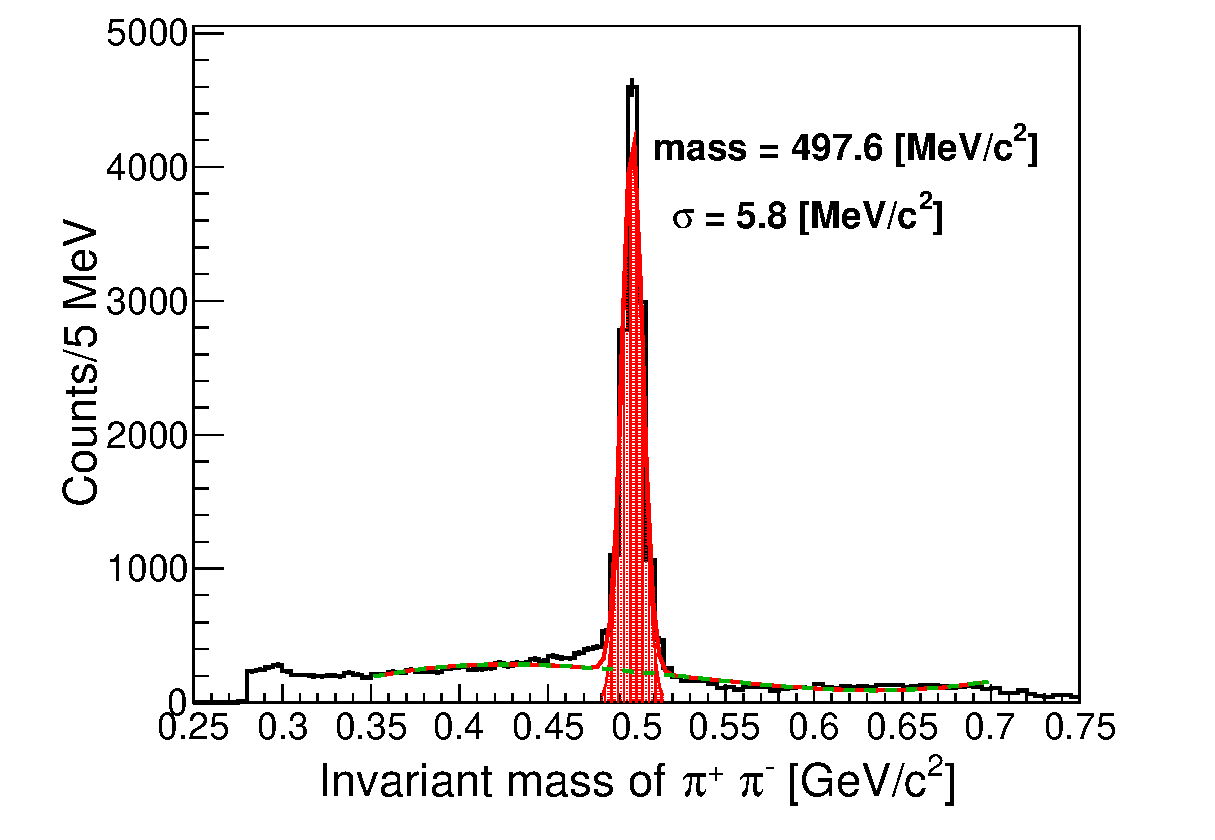
\includegraphics[width=4.5cm]{../pic/Run78/KN_ana_NC170_3sigma/IM_pipi_fitGauss.eps}
    \end{minipage}

    \begin{minipage}{0.33\hsize}
      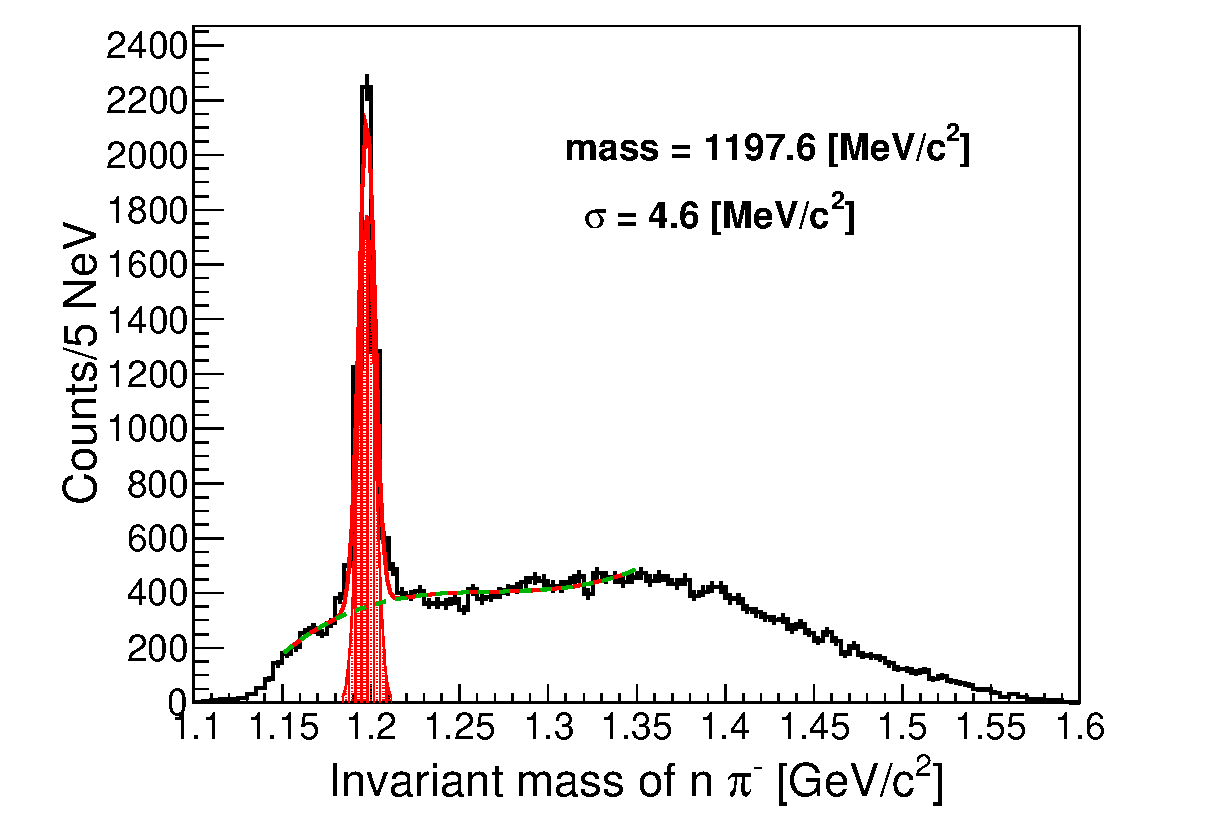
\includegraphics[width=4.5cm]{../pic/Run78/KN_ana_NC170_3sigma/IM_npim_fitGauss.eps}
    \end{minipage}

    \begin{minipage}{0.33\hsize}
      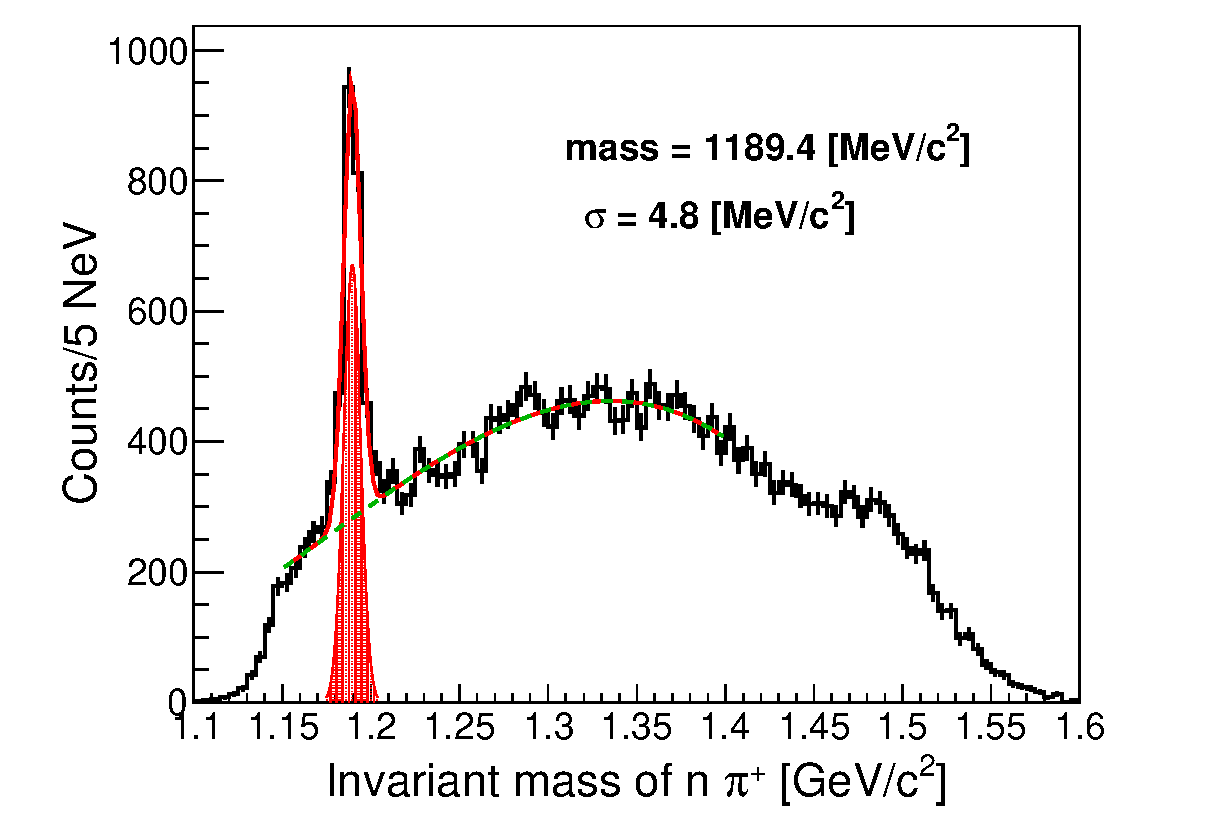
\includegraphics[width=4.5cm]{../pic/Run78/KN_ana_NC170_3sigma/IM_npip_fitGauss.eps}
    \end{minipage}
  \end{tabular}
  \caption{
    These figures show the invariant mass distributions of $\pi^+ \pi^-$,
    $n \pi^-$ and $n \pi^+$ in the $K d \rightarrow n \pi^+ \pi^- n$ event sample from left to right.
    The Gaussian functions and the selection regions for $K^0$ and $\Sigma^{\pm}_{forward}$ are indicated by red hatched area.
    The background third-order polynomial functions are shown as the green dashed lines.
  }
  \label{fig:npipin_IM_fitGauss}
\end{figure}


Rejecting these two reactions leaves a signal reaction in which $\pi \Sigma$ is scattered backward.
This reaction has $\pi^- \Sigma^+$ and $\pi^+ \Sigma^-$ modes, and they must be separated.
The branching ratio of these modes depends on the mass of $\pi \Sigma$, and this separation is performed for each bin of $d(K^-, n)$ missing mass.

\begin{frame}{$d(K^-, n)"nK0"$}
  \begin{figure}
    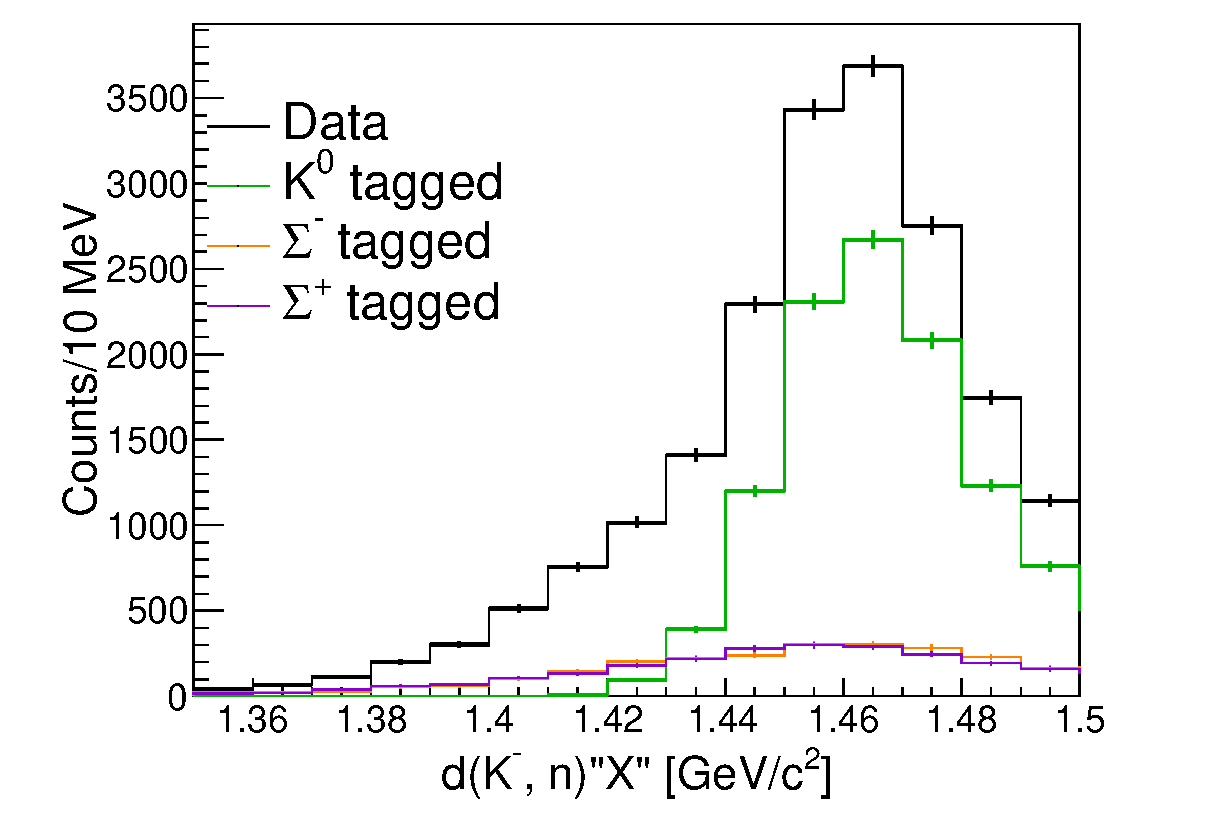
\includegraphics[width=8cm]{../pic/Run78/KN_ana_NC170_2sigma/KN_MM_all.eps}
  \end{figure}
\end{frame}


Figure \ref{fig:KN_MM_npipin} shows the $d(K^-, n)$ missing masses in which the $K^- d \rightarrow n \pi^+ \pi^- n$ final state has been identified.
On the left, all events, those identifying $K^0$, those identifying $\Sigma^+_{forward}$, and those identifying $\Sigma^-_{forward}$
are indicated by black, green, red, and blue lines, respectively.
The right figure shows the signal spectrum, subtracting the events identified as $K^0$ or $\Sigma^{\pm}_{forward}$ from all events.

To separate these events,
we generated template events using a Geant4 Monte Carlo simulation and decomposed the reactions by fitting their spectra with templates.
This decomposition was applied not only to the signal but also to the background reactions.
The procedures used in this decomposition are described in detail in Section \ref{sec:template_fitting}
The estimation of the detector resolution used in this simulation is described in detail in Appendix \ref{chapter:detector_resolution}.



\subsection{Template fitting} \label{sec:template_fitting}
\newcommand{\IMfitChiSquare}{1077.4}
\newcommand{\IMfitNDF}{352}
\newcommand{\IMfitChiNDF}{3.06}

\newcommand{\KzeroFitChi}{275.2}
\newcommand{\KzeroFitNDF}{43}
\newcommand{\KzeroFitChiNDF}{6.40}

\newcommand{\KzeroOneStepRatio}{80.9 \pm 1.3\%}
\newcommand{\KzeroTwoStepRatio}{11.5 \pm 1.0\%}
\newcommand{\KzeroLsRatio}{7.7 \pm 0.6\%}


% \section{Template fitting of $K^- d \rightarrow n \pi^+ \pi^- n$ events} \label{sec:tempFit}
% \subsection{Backward $\pi^{\mp}\Sigma^{\pm}$ event selection} \label{sec:backward_piSigma}
\begin{figure}
  \centering
  \begin{tikzpicture}[scale=1.2]
    \draw (-1.5,    1) node {$K^-$}--(0,    0);
    \draw (-1.5,    0)--(0,    0);
    \draw (-1.5, -0.2)--(0.3, -0.2);
    \node (d) at (-1.5, -0.1) [left] {$d$};

    \draw (0, 0) -- (0.3, -0.2) [dashed];
    \node (barK) at (0.3, -0.15) [above] {$\bar{K}$};

    \draw ( 1.5,  1.0) node [right] {\textcolor{red}{$n$ detected}}      -- (0,    0);
    
    \draw ( 1.5,  -0.7) node [right] {\textcolor{blue}{$\pi$ detected}} -- (0.3, -0.2);
    
    \draw ( 0.8,  -0.15) node [above] {$\Sigma$}    -- (0.3, -0.2);
    \draw ( 0.8,  -0.15) -- (1.5, 0.1) node [right] {$n$ missing};
    \draw ( 0.8,  -0.15) -- (1.5, -0.3) node [right] {\textcolor{blue}{$\pi$ detected}};    
  \end{tikzpicture}\\
  (a)
  
  \begin{tabular}{cc}
    \begin{minipage}{0.5\hsize}
      \centering
      \begin{tikzpicture}[scale=1.2]
        \draw (-1.5,    1) node {$K^-$}--(0,    0);
        \draw (-1.5,    0)--(0,    0);
        \draw (-1.5, -0.2)--(0, -0.2);
        \node (d) at (-1.5, -0.1) [left] {$d$};
        
        \draw ( 1.5,  1.0) node [right] {\textcolor{red}{$n$ detected}}      -- (0,    0);

        
        \node (K0) at (0.5, -0.4) [below] {$K^0$};
        \draw (0, -0.1) -- (0.7, -0.45);
        
        \draw ( 0.0,  -0.15) -- (1.5, 0.1) node [right] {$n$ missing};
        \draw ( 0.7,  -0.45) -- (1.5, -0.3) node [right] {\textcolor{blue}{$\pi$ detected}};
        \draw (1.5,  -0.7) node [right] {\textcolor{blue}{$\pi$ detected}} -- (0.7, -0.45);
        
        \filldraw [fill=white] (0, -0.1) circle [radius=0.15];
      \end{tikzpicture}\\
      (b)
    \end{minipage}
    \begin{minipage}{0.5\hsize}
      \centering
      \begin{tikzpicture}[scale=1.2]
        \draw (-1.5,    1) node {$K^-$}--(0,    0);
        \draw (-1.5,    0)--(0,    0);
        \draw (-1.5, -0.2)--(0.3, -0.2);
        \node (d) at (-1.5, -0.1) [left] {$d$};

        \draw ( 1.5,  -0.2) node [right] {n missing} -- (0.3, -0.2);
        \draw ( 1.5,  0.3) node [right] {\textcolor{blue}{$\pi$ detected}}      -- (0,    0);

        \node (barK) at (0.4, 0.4) [above] {$\Sigma$};
        \draw ( 0.7,  0.6) -- (0.0, 0.0);
                
        \draw ( 0.7,  0.6) -- (1.5, 1.5) node [right] {\textcolor{red}{$n$ detected}};
        \draw ( 0.7,  0.6) -- (1.5, 1.0) node [right] {\textcolor{blue}{$\pi$ detected}};    
      \end{tikzpicture}\\
      (c)
    \end{minipage}
  \end{tabular}
  \label{fig:kd_npipin_type}
\end{figure}


The $K^- n \rightarrow n \pi^+ \pi^- n$ final state is identified from the event in which the forward neutron is detected,
as described in Section.\ref{sec:???}.
This final state can be considered to include the three reactions represented in Figure \ref{fig:kd_npipin_type}.
The first is the signal reaction in this analysis where $\bar{K}$ is recoiled backward to $\pi \Sigma$
as shown in Figure.\ref{fig:kd_npipin_type}-(a),
the second is the recoil of $K^0$ decaying directly to $\pi^+ \pi^-$ as shown in Figure \ref{fig:kd_npipin_type}-(b),
and the third is the forward production of $\Sigma$ ($\Sigma_{forward}$) as shown in Figure \ref{fig:kd_npipin_type}-(c),
where forward means that the $n$ decaying from $\Sigma$ are detected by the NC.
Reactions (b) and (c) can be identified by reconstructing $K^0$ and $\Sigma^{\pm}$
from the invariant masses of $\pi^+$ and $\pi^-$ and forward neutrons and $\pi^{\pm}$, respectively,
as shown in Figure.\ref{fig:npipin_IM_fitGauss}.
The invariant mass distributions of $\pi^+ \pi^-$, $n \pi^-$ and $n \pi^+$ are represented in the right, center and left figures respectively.
For the identification of $K^0$ and $\Sigma^{\pm}_{forward}$,
fitting with third-order polynomial function and Gaussian function is used to identify $K^0$ and $\Sigma^{\pm}_{forward}$
in the 3$\sigma$ region of the Gaussian function, which is indicated by the red hatched area.

\begin{figure}[htbp]
  \begin{tabular}{ccc}
    \begin{minipage}{0.33\hsize}
      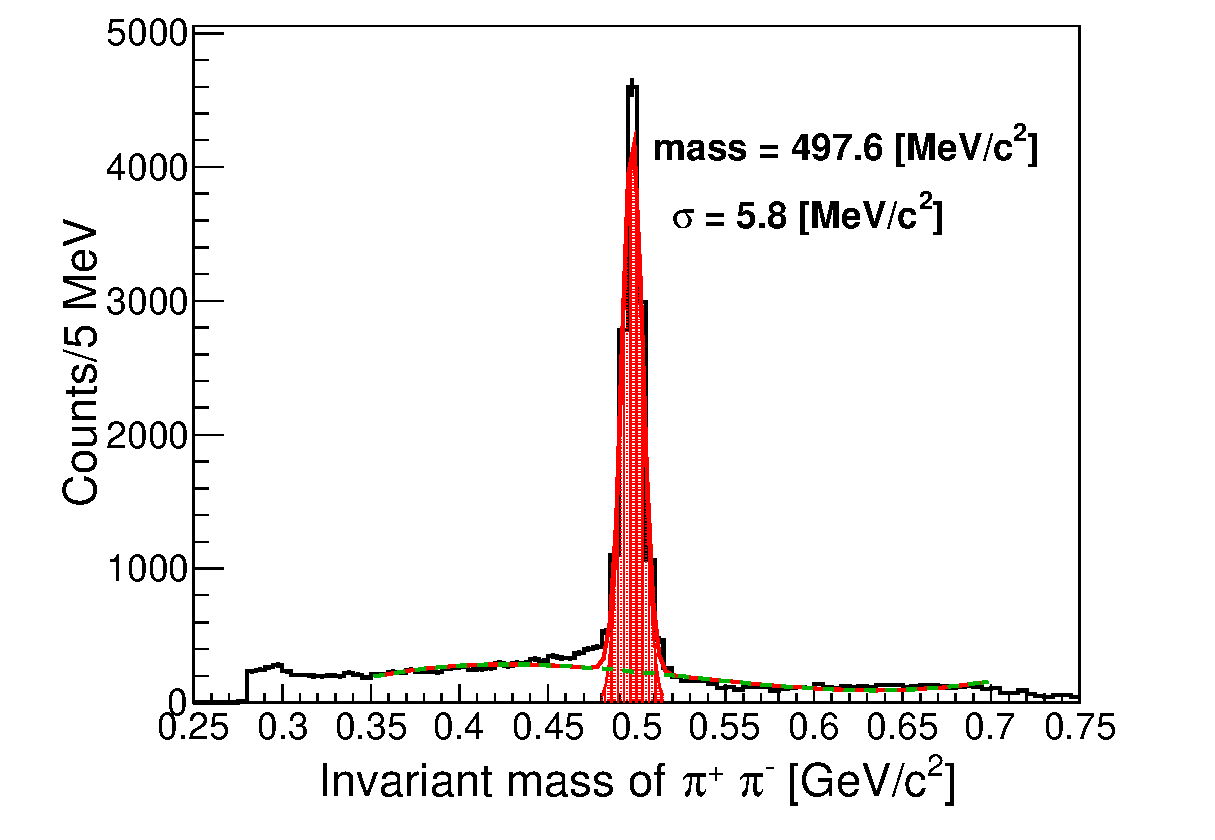
\includegraphics[width=4.5cm]{../pic/Run78/KN_ana_NC170_3sigma/IM_pipi_fitGauss.eps}
    \end{minipage}

    \begin{minipage}{0.33\hsize}
      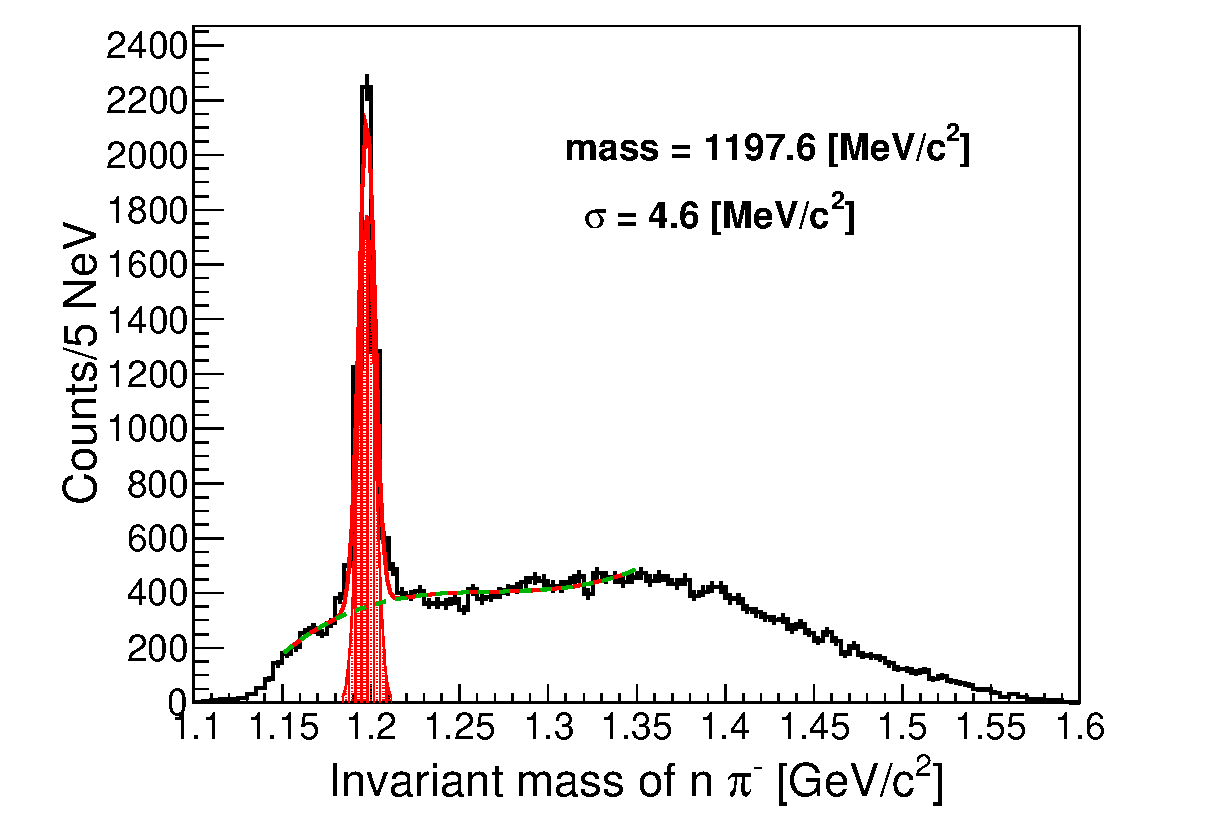
\includegraphics[width=4.5cm]{../pic/Run78/KN_ana_NC170_3sigma/IM_npim_fitGauss.eps}
    \end{minipage}

    \begin{minipage}{0.33\hsize}
      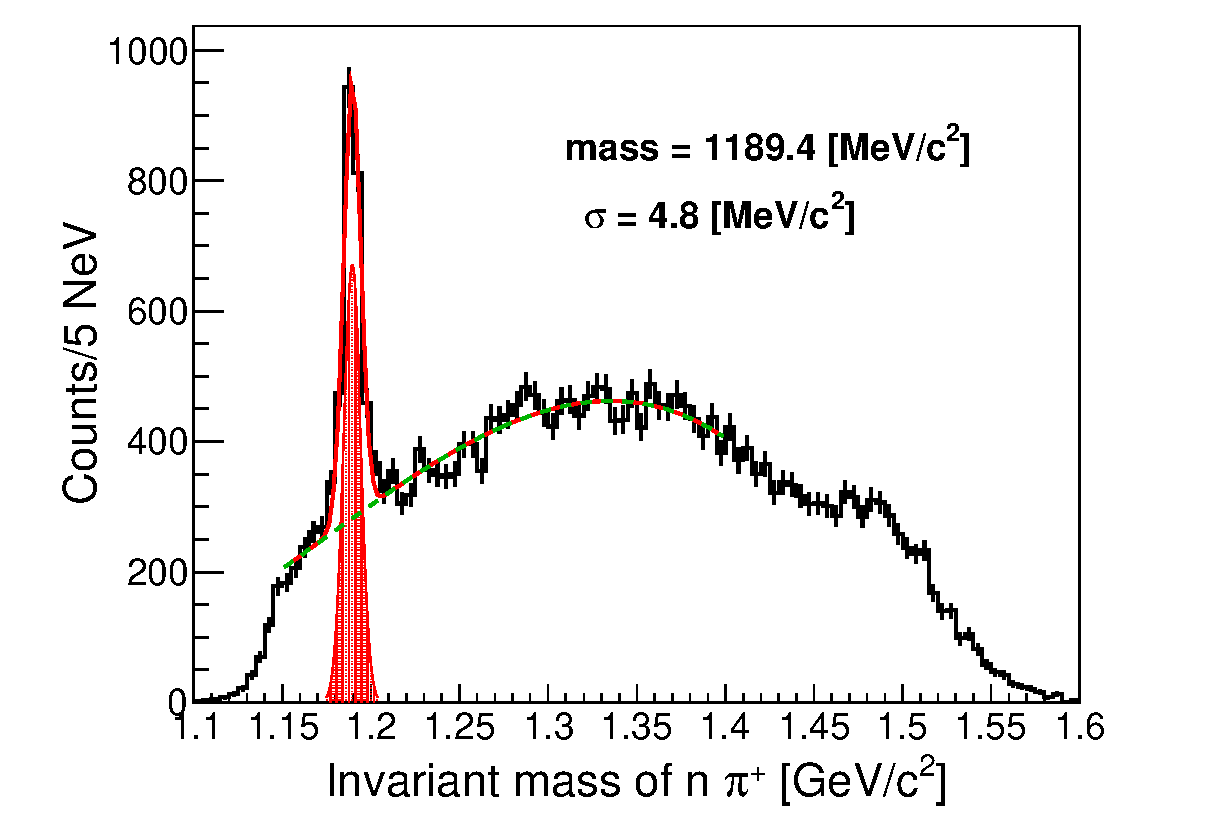
\includegraphics[width=4.5cm]{../pic/Run78/KN_ana_NC170_3sigma/IM_npip_fitGauss.eps}
    \end{minipage}
  \end{tabular}
  \caption{
    These figures show the invariant mass distributions of $\pi^+ \pi^-$,
    $n \pi^-$ and $n \pi^+$ in the $K d \rightarrow n \pi^+ \pi^- n$ event sample from left to right.
    The Gaussian functions and the selection regions for $K^0$ and $\Sigma^{\pm}_{forward}$ are indicated by red hatched area.
    The background third-order polynomial functions are shown as the green dashed lines.
  }
  \label{fig:npipin_IM_fitGauss}
\end{figure}


Rejecting these two reactions leaves a signal reaction in which $\pi \Sigma$ is scattered backward.
This reaction has $\pi^- \Sigma^+$ and $\pi^+ \Sigma^-$ modes, and they must be separated.
The branching ratio of these modes depends on the mass of $\pi \Sigma$, and this separation is performed for each bin of $d(K^-, n)$ missing mass.

\begin{frame}{$d(K^-, n)"nK0"$}
  \begin{figure}
    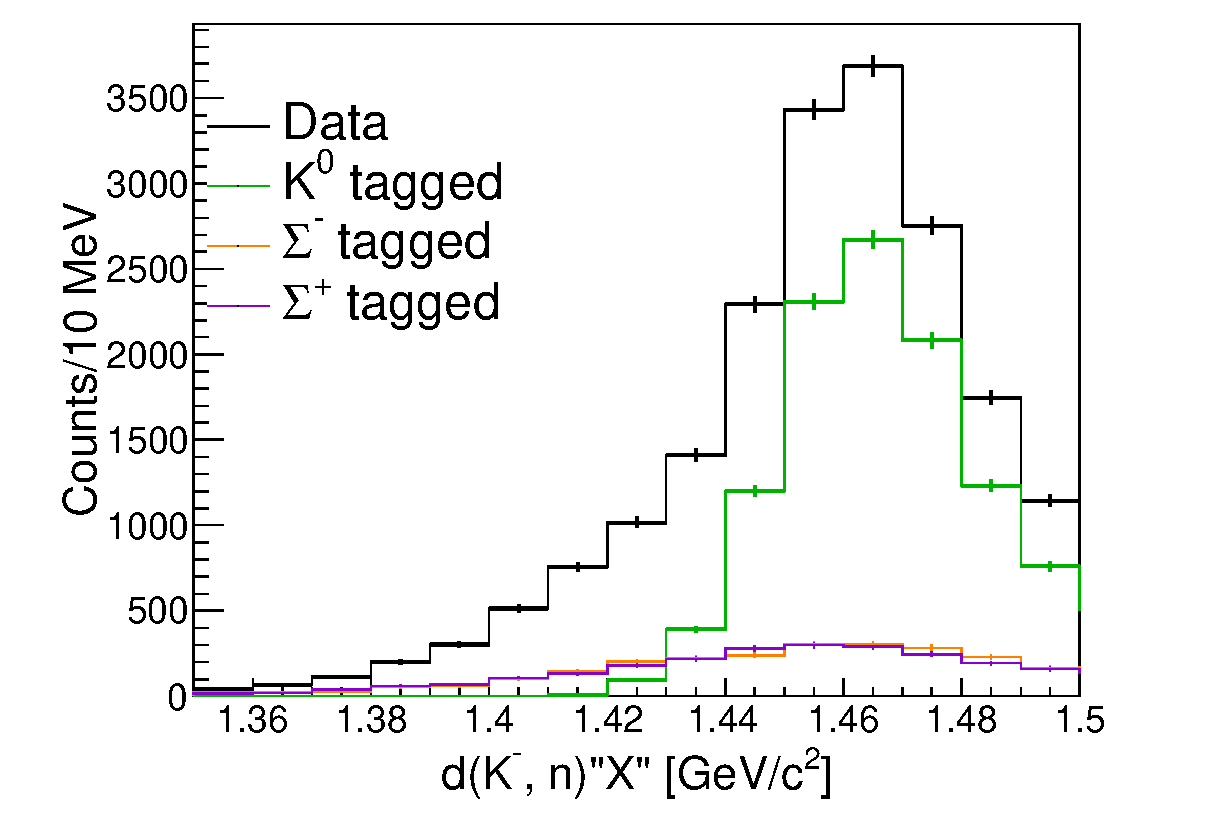
\includegraphics[width=8cm]{../pic/Run78/KN_ana_NC170_2sigma/KN_MM_all.eps}
  \end{figure}
\end{frame}


Figure \ref{fig:KN_MM_npipin} shows the $d(K^-, n)$ missing masses in which the $K^- d \rightarrow n \pi^+ \pi^- n$ final state has been identified.
On the left, all events, those identifying $K^0$, those identifying $\Sigma^+_{forward}$, and those identifying $\Sigma^-_{forward}$
are indicated by black, green, red, and blue lines, respectively.
The right figure shows the signal spectrum, subtracting the events identified as $K^0$ or $\Sigma^{\pm}_{forward}$ from all events.

To separate these events,
we generated template events using a Geant4 Monte Carlo simulation and decomposed the reactions by fitting their spectra with templates.
This decomposition was applied not only to the signal but also to the background reactions.
The procedures used in this decomposition are described in detail in Section \ref{sec:template_fitting}
The estimation of the detector resolution used in this simulation is described in detail in Appendix \ref{chapter:detector_resolution}.



\subsection{Template fitting} \label{sec:template_fitting}
\newcommand{\IMfitChiSquare}{1077.4}
\newcommand{\IMfitNDF}{352}
\newcommand{\IMfitChiNDF}{3.06}

\newcommand{\KzeroFitChi}{275.2}
\newcommand{\KzeroFitNDF}{43}
\newcommand{\KzeroFitChiNDF}{6.40}

\newcommand{\KzeroOneStepRatio}{80.9 \pm 1.3\%}
\newcommand{\KzeroTwoStepRatio}{11.5 \pm 1.0\%}
\newcommand{\KzeroLsRatio}{7.7 \pm 0.6\%}


% \section{Template fitting of $K^- d \rightarrow n \pi^+ \pi^- n$ events} \label{sec:tempFit}
% \subsection{Backward $\pi^{\mp}\Sigma^{\pm}$ event selection} \label{sec:backward_piSigma}
\input{analysis/template_fitting/figs/kd_npipin_type}

The $K^- n \rightarrow n \pi^+ \pi^- n$ final state is identified from the event in which the forward neutron is detected,
as described in Section.\ref{sec:???}.
This final state can be considered to include the three reactions represented in Figure \ref{fig:kd_npipin_type}.
The first is the signal reaction in this analysis where $\bar{K}$ is recoiled backward to $\pi \Sigma$
as shown in Figure.\ref{fig:kd_npipin_type}-(a),
the second is the recoil of $K^0$ decaying directly to $\pi^+ \pi^-$ as shown in Figure \ref{fig:kd_npipin_type}-(b),
and the third is the forward production of $\Sigma$ ($\Sigma_{forward}$) as shown in Figure \ref{fig:kd_npipin_type}-(c),
where forward means that the $n$ decaying from $\Sigma$ are detected by the NC.
Reactions (b) and (c) can be identified by reconstructing $K^0$ and $\Sigma^{\pm}$
from the invariant masses of $\pi^+$ and $\pi^-$ and forward neutrons and $\pi^{\pm}$, respectively,
as shown in Figure.\ref{fig:npipin_IM_fitGauss}.
The invariant mass distributions of $\pi^+ \pi^-$, $n \pi^-$ and $n \pi^+$ are represented in the right, center and left figures respectively.
For the identification of $K^0$ and $\Sigma^{\pm}_{forward}$,
fitting with third-order polynomial function and Gaussian function is used to identify $K^0$ and $\Sigma^{\pm}_{forward}$
in the 3$\sigma$ region of the Gaussian function, which is indicated by the red hatched area.

\input{analysis/template_fitting/figs/npipin_IM_fitGauss}

Rejecting these two reactions leaves a signal reaction in which $\pi \Sigma$ is scattered backward.
This reaction has $\pi^- \Sigma^+$ and $\pi^+ \Sigma^-$ modes, and they must be separated.
The branching ratio of these modes depends on the mass of $\pi \Sigma$, and this separation is performed for each bin of $d(K^-, n)$ missing mass.

\input{analysis/template_fitting/figs/KN_MM}

Figure \ref{fig:KN_MM_npipin} shows the $d(K^-, n)$ missing masses in which the $K^- d \rightarrow n \pi^+ \pi^- n$ final state has been identified.
On the left, all events, those identifying $K^0$, those identifying $\Sigma^+_{forward}$, and those identifying $\Sigma^-_{forward}$
are indicated by black, green, red, and blue lines, respectively.
The right figure shows the signal spectrum, subtracting the events identified as $K^0$ or $\Sigma^{\pm}_{forward}$ from all events.

To separate these events,
we generated template events using a Geant4 Monte Carlo simulation and decomposed the reactions by fitting their spectra with templates.
This decomposition was applied not only to the signal but also to the background reactions.
The procedures used in this decomposition are described in detail in Section \ref{sec:template_fitting}
The estimation of the detector resolution used in this simulation is described in detail in Appendix \ref{chapter:detector_resolution}.



\subsection{Template fitting} \label{sec:template_fitting}
\input{discussion/template_fitting/params}

% \section{Template fitting of $K^- d \rightarrow n \pi^+ \pi^- n$ events} \label{sec:tempFit}
% \subsection{Backward $\pi^{\mp}\Sigma^{\pm}$ event selection} \label{sec:backward_piSigma}
\input{discussion/template_fitting/backward_piSigma_selection}

\subsection{Template fitting} \label{sec:template_fitting}
\input{discussion/template_fitting/template_fitting}

%% \input{discussion/template_fitting/MC_data}
%% \input{discussion/template_fitting/procedure}
%% \input{discussion/template_fitting/fit_K0}



%% \subsection{Generated data by Monte Calro simulation} \label{subsec:tempFit_MCdata}
\input{discussion/template_fitting/reactions}
Since the $K^- d\rightarrow n \pi^+ \pi^- n$ event is expected to contain 3 type reactions, (\ref{reaction:prodK0})-(\ref{2step:piS}),
we obtain the $d(K^-, n)"\pi^{\mp}\Sigma^{\pm}"$ event rejecting $K^0$ and $\Sigma^{\pm}_{forward}$ in $K^- d \rightarrow n \pi^+ \pi^- n$ event.

We perform template fitting using data reproduced using Monte Carlo simulation (geant4) to decompose into $\pi^-\Sigma^+$ and $\pi^+\Sigma^-$ modes.
In this subsection, we explain how we reproduce the data using geant4 simulation.

The $K^0$ production in (\ref{reaction:prodK0}) is simply the so-called quasi-elastic scattering,
in which an initial $K^-$ reacts with a proton and is converted into $K^0$ and a neutron, where the residual neutron is a spectator and its momentum is the Fermi momentum.
This reaction causes the scattering angles of the reacting protons and $K^-$ to be distributed in a way that reproduces the past experiment of one nucleon scattering \cite{KP_K0n},
and the momentum of the spectator is also distributed in a way that reproduces the past experiment \cite{d_fermi_ex}.
In the case of $\Sigma^{\pm}_{forward}$ production in (\ref{reaction:prodSigma}), the angular distribution of the past experiment\cite{KP_CEX_1GeV} is simulated in the same way.

In the $K^0$ produced event (\ref{reaction:prodK0}), in addition to 1-step reaction described above, events such as a 2-step and direct $\Lambda(1520)$ production are observed.
So, we generate data of these reaction.
In the case of 2-step reaction, the momentum of recoiled $\bar{K}$ is small and the scattering data of such $\bar{K}$ and nucleon are a few,
so the angular distribution and other details are not known.
Therefore, the MC data is generated assuming that the scattering of recoiled $\bar{K}$ and nucleons is isotropic. 
In the case of direct $\Lambda(1520)$ production also no data.
Therefore, this data was isotropically scattered $K^-d \rightarrow n \Lambda(1520)$ and $\Lambda(1520)$ decayed to $n$ and $K^0$.

Next, we explain the main signal (\ref{2step:piS}), which is the backward $\pi\Sigma$ generation.
Since there is no data on the invariant mass of $\pi\Sigma$, it is generated as a uniform distribution from the $\bar{K}N$ threshold, whose lineshape is determined by template fitting.
There is also no data on the scattering angle of $\pi\Sigma$,
but since the $\bar{K}N\rightarrow \pi\Sigma$ scattering is expected to be $S$-wave in this reaction,
we assume that it is isotropic and generate MC data.

In summary, the following seven MC data are used for template fitting.
\input{discussion/template_fitting/MC_data_list}

%% \subsection{Procedure of template fitting}
\input{discussion/template_fitting/figs/fit_IM}
\input{discussion/template_fitting/figs/fit_KNpi_MM_all}

In this subsection, we explain procedure of template fitting, whose main purpose is decomposition of $\pi^- \Sigma^+$ and $\pi^+ \Sigma^-$ modes.
Template fitting is divided into two stages, one fitting to estimate the amount of background for $K^0$ and $\Sigma_{forward}$ production,
the other to separate $\pi^-\Sigma^+$ and $\pi^+\Sigma^-$ modes.
These fittings are performed using fitting with the likelihood method on a finite sample generated by Monte Carlo method\cite{temp_fit}.
There is no $\chi^2$ in this fitting,
but there is a value of $-2\log\Lambda$ that asymptotically approaches the $\chi^2$ when the number of samples become infinite, and the fitting is evaluated with this value.
Here, $\Lambda$ is the likelihood.

The first fitting is performed using the invariant mass distributions of $\pi^+ \pi^-$, $n \pi^+$ and $n \pi^-$ in the event that $K^-d \rightarrow n \pi^+ \pi^- n$ final state.
The $K^0$, $\Sigma^+$ and $\Sigma^-$ productions create peaks in the respective invariant mass distributions as shown in Fig.\ref{fig:fit_IM}.
The distributions reconstructed by fitting are also plotted in the same figure.
The bold line represents the case of backward $\pi \Sigma$ production of signal, with red and blue representing the $\pi^- \Sigma^+$ and $\pi^-\Sigma^+$ modes, respectively.
The other green, purple and orange lines represent the background for $K^0$, $\Sigma^-_{forward}$ and $\Sigma^+_{forward}$ production, respectively.
This fitting of $-2\log\Lambda$ is \IMfitChiSquare.
Degrees freedom is the number of bin with data, and $-2\log\Lambda/NDF \sim $\IMfitChiNDF. 
% For this purpose, the distribution is fitted with a Gaussian and a 5-th polynomial function, and the rejection region is defined by the 3$\sigma$ of the Gaussian.

\input{discussion/template_fitting/figs/fit_KNpi_MM}
\input{discussion/template_fitting/figs/tempFit_KNpi_Chi2}

The fitting to separate the $\pi^-\Sigma^+$ and $\pi^+\Sigma^-$ modes is performed for events from $K^-- d \rightarrow n \pi^+ \pi- n$, excluding $K^0 $and $\Sigma^{\pm}_{forward}$ production.
However, the background leakage is estimated by scaling the distribution reconstructed in the MC simulation by the intensity estimated by the invariant mass fitting.
This fitting is performed each bin of the missing mass of $d(K^-, n)$, since the scattering amplitude of $\bar{K}N \rightarrow \pi \Sigma$ depends on the $\pi \Sigma$ invariant mass.
For this fitting we use the $d(K^-, n \pi^-)$ and $d(K^-, n \pi^+)$ missing masses as shown in Fig.\ref{fig:fit_KNpi_MM_all}.
This figure shows the sum of the $d(K^- , n)$ bins.
The bottom left figure shows a two-dimensional figure of the $d(K^-, n \pi^-)$ and $d(K^-, n \pi^+)$ missing masses on the horizontal and vertical axes, respectively.
The top and right figures show the projections of the respective axes.
The missing mass of $d(K^-, n \pi)$ makes a peak at $\Sigma$ for the correct combination for the missing $\Sigma$, but is widely distributed in the kinematic region for the opposite charge.
For example, for $d(K^-, n \pi^-)$, the $\pi^- \Sigma^+$ mode has a peak structure as shown by the red line,
whereas the $\pi^+ \Sigma^-$ mode has a widely distributed structure as shown by the blue line.

Fig.\ref{fig:fit_KNpi_MM} shows the results for the fitting of each bin of $d(K^-, n)$ separately.
Fig.\ref{fig:tempFit_KNpi_Chi2} shows the $-2\log\Lambda$ and $-2\log\Lambda/NDF$ of this fitting in each $d(K^-, n)$ bin in black and red, respectively.

Fitting to estimate background and to separate $\pi^- \Sigma^+$ and $\pi^+ \Sigma^-$ modes cannot be performed simultaneously as they use different event samples.
They are therefore repeated in the following steps.

First, the separation of $\pi^- \Sigma^+$ and $\pi^+ \Sigma^-$ modes is performed without considering the background.
The obtained distribution of backward $\pi^{\mp} \Sigma^{\pm}$ modes is used for fitting to estimate the background,
which is then fed back into the fitting of the separation of $\pi^- \Sigma^+$ and $\pi^+ \Sigma^-$ modes.
After five iterations of this procedure, fitting is performed considering 2-step and direct $\Lambda(1520)$ generation for $K^0$ generation, which is described in the Appendix.\ref{apendix:K0_event}.
Finally, fitting of the separation of the $\pi^- \Sigma^+$ and $\pi^+ \Sigma^-$ modes is performed to obtain the final $\pi \Sigma$ spectrum as shown in Fig.\ref{fig:piS_num}..

\input{discussion/template_fitting/figs/piS_num}


%% \begin{frame}{Template fitting to decompose $K^0$ production}
  \begin{figure}
    \centering
    Invariant mass of $n K^0$\\
    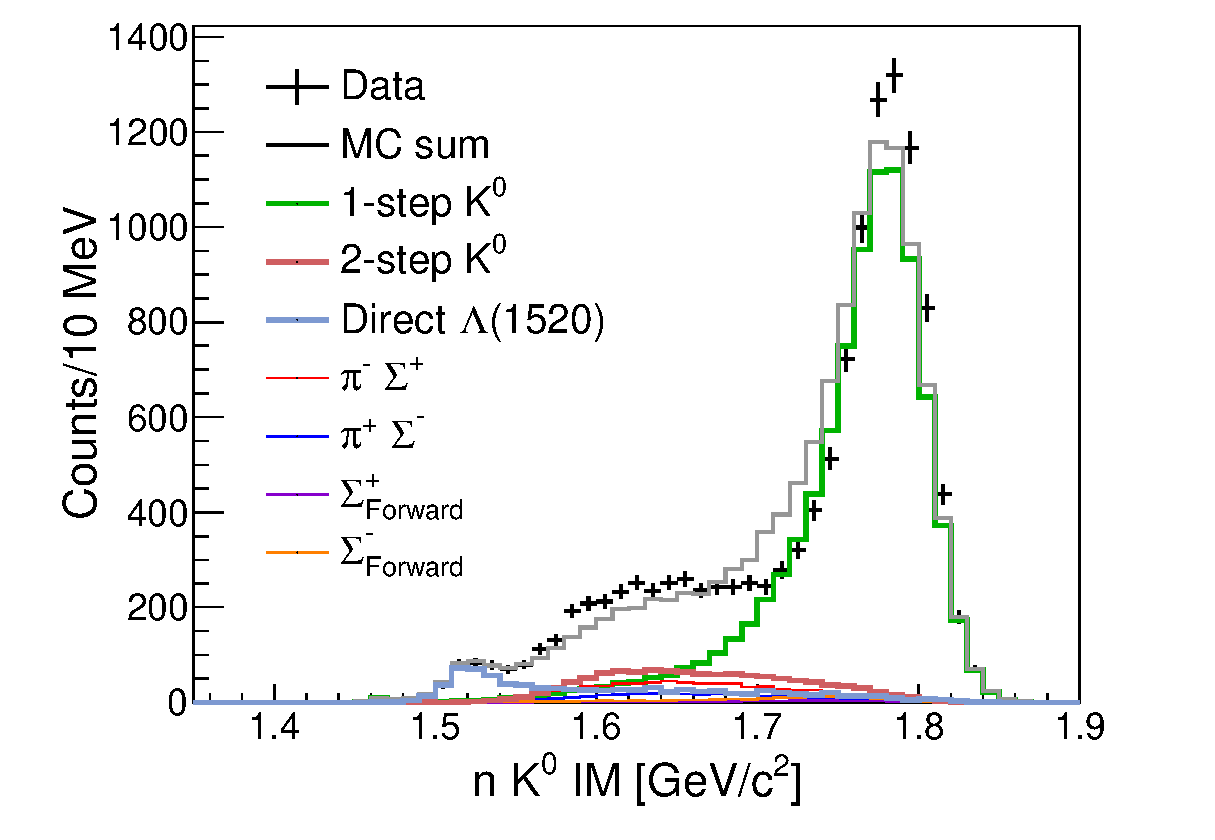
\includegraphics[width=7.5cm]{../pic/Dron/K0_ana/npipi_IM_K0.eps}
  \end{figure}
  \centering
  2-step like component is seen about 11.5\%.\\
  Direct-$\Lambda(1520)$ prod. is seen about 7.7\%.\\
\end{frame}




%% \subsection{Generated data by Monte Calro simulation} \label{subsec:tempFit_MCdata}
\begin{eqnarray}
  & &  K^- d \rightarrow n K^0 n \label{reaction:prodK0} \\
  & &  K^- d \rightarrow \pi^\mp \Sigma^\pm n_{forward} \label{2step:piS}\\
  & &  K^- d \rightarrow \pi^\mp \Sigma^\pm n_{missing} \label{reaction:prodSigma}
\end{eqnarray}

Since the $K^- d\rightarrow n \pi^+ \pi^- n$ event is expected to contain 3 type reactions, (\ref{reaction:prodK0})-(\ref{2step:piS}),
we obtain the $d(K^-, n)"\pi^{\mp}\Sigma^{\pm}"$ event rejecting $K^0$ and $\Sigma^{\pm}_{forward}$ in $K^- d \rightarrow n \pi^+ \pi^- n$ event.

We perform template fitting using data reproduced using Monte Carlo simulation (geant4) to decompose into $\pi^-\Sigma^+$ and $\pi^+\Sigma^-$ modes.
In this subsection, we explain how we reproduce the data using geant4 simulation.

The $K^0$ production in (\ref{reaction:prodK0}) is simply the so-called quasi-elastic scattering,
in which an initial $K^-$ reacts with a proton and is converted into $K^0$ and a neutron, where the residual neutron is a spectator and its momentum is the Fermi momentum.
This reaction causes the scattering angles of the reacting protons and $K^-$ to be distributed in a way that reproduces the past experiment of one nucleon scattering \cite{KP_K0n},
and the momentum of the spectator is also distributed in a way that reproduces the past experiment \cite{d_fermi_ex}.
In the case of $\Sigma^{\pm}_{forward}$ production in (\ref{reaction:prodSigma}), the angular distribution of the past experiment\cite{KP_CEX_1GeV} is simulated in the same way.

In the $K^0$ produced event (\ref{reaction:prodK0}), in addition to 1-step reaction described above, events such as a 2-step and direct $\Lambda(1520)$ production are observed.
So, we generate data of these reaction.
In the case of 2-step reaction, the momentum of recoiled $\bar{K}$ is small and the scattering data of such $\bar{K}$ and nucleon are a few,
so the angular distribution and other details are not known.
Therefore, the MC data is generated assuming that the scattering of recoiled $\bar{K}$ and nucleons is isotropic. 
In the case of direct $\Lambda(1520)$ production also no data.
Therefore, this data was isotropically scattered $K^-d \rightarrow n \Lambda(1520)$ and $\Lambda(1520)$ decayed to $n$ and $K^0$.

Next, we explain the main signal (\ref{2step:piS}), which is the backward $\pi\Sigma$ generation.
Since there is no data on the invariant mass of $\pi\Sigma$, it is generated as a uniform distribution from the $\bar{K}N$ threshold, whose lineshape is determined by template fitting.
There is also no data on the scattering angle of $\pi\Sigma$,
but since the $\bar{K}N\rightarrow \pi\Sigma$ scattering is expected to be $S$-wave in this reaction,
we assume that it is isotropic and generate MC data.

In summary, the following seven MC data are used for template fitting.
\begin{itemize}
  \item About $K^0$ production reaction
  \begin{itemize}
  \item
    $ K^- d \rightarrow n_{forward} K^0 n_{spectator}$ \hspace{\fill} ($K^0$ 1-step)
  \item
    $K^- d \rightarrow n_{forward} (K^0 n)_{isotropic}$ \hspace{\fill} ($K^0$ 2-step)
  \item
    $K^- d \rightarrow n \Lambda(1520) \rightarrow n K^0 n$ \hspace{\fill} (direct $\Lambda(1520)$)
  \end{itemize}
\item About $\Sigma_{forward}$ production reaction
  \begin{itemize}
  \item
    $K^- d \rightarrow \Sigma^+ \pi^- n_{spectator} \rightarrow n_{forward} \pi^+ \pi^- n_{spectator}$ \hspace{\fill} ($\Sigma^+$ 1-step)
  \item
    $K^- d \rightarrow \Sigma^- \pi^+ n_{spectator} \rightarrow n_{forward} \pi^- \pi^+ n_{spectator}$ \hspace{\fill} ($\Sigma^-$ 1-step)
  \end{itemize}
\item About backward $\pi \Sigma$ production reaction
  \begin{itemize}
  \item
    $K^- d \rightarrow n_{forward} \pi^- \Sigma^+$ \hspace{\fill} (backward $\pi^- \Sigma^+$)
  \item
    $K^- d \rightarrow n_{forward} \pi^+ \Sigma^-$ \hspace{\fill} (backward $\pi^+ \Sigma^-$)
  \end{itemize}
\end{itemize}


%% \subsection{Procedure of template fitting}
\begin{frame}{Template fitting to evaluate background}
  \centering
  $d(K^, n \pi^- \pi^+)"n"$ event.
  \begin{tabular}{ccc}
    \begin{minipage}{0.33\hsize}
      \centering
      $\pi^+ \pi^-$ IM\\
      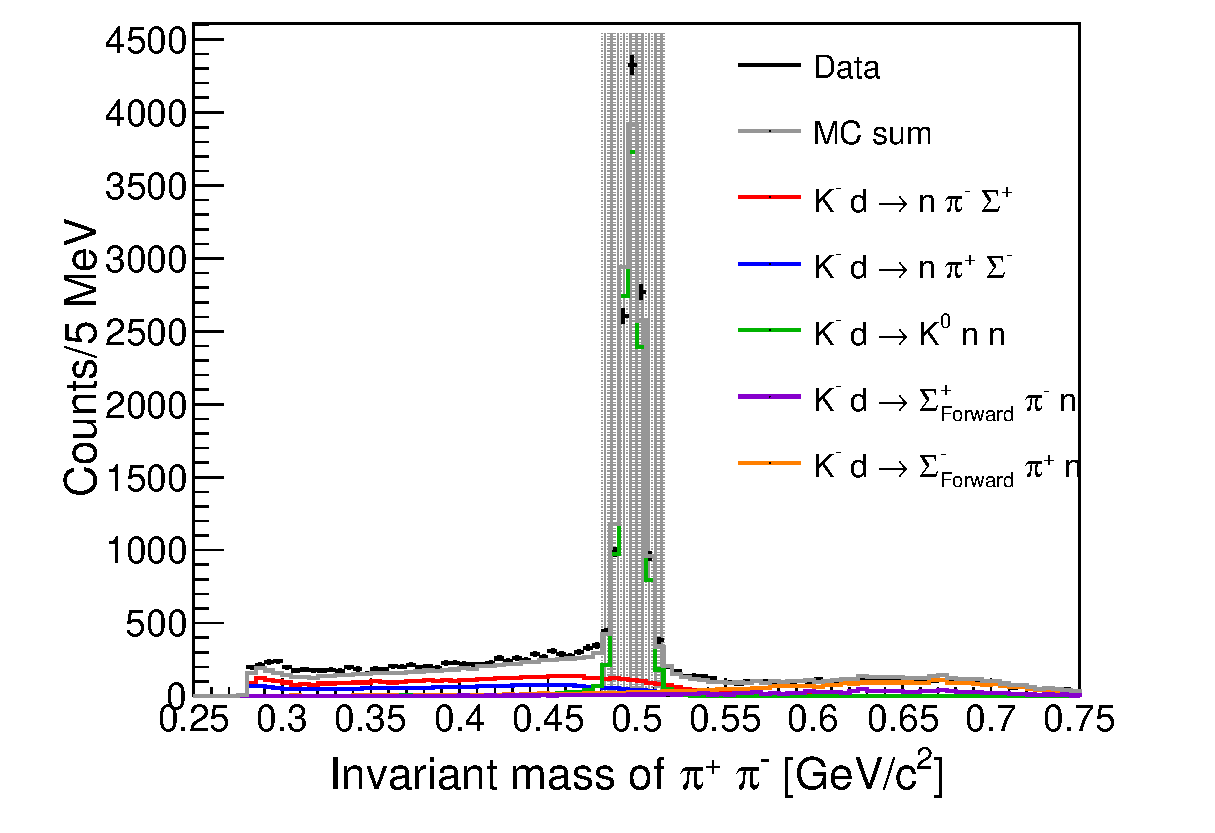
\includegraphics[width=4cm]{../pic/Dron/KN_ana/IM_pipi.eps}
    \end{minipage}
    \begin{minipage}{0.33\hsize}
      \centering
      $n_{forward} \pi^+$ IM\\
      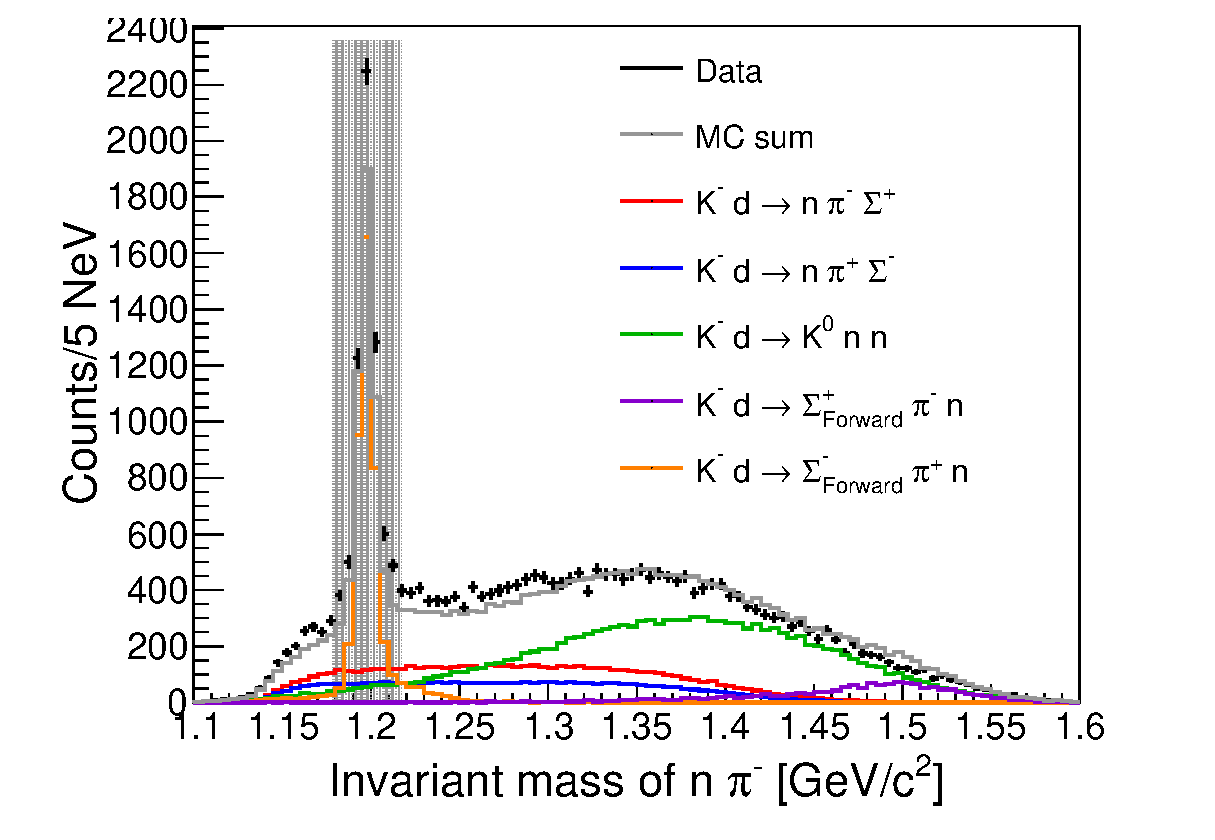
\includegraphics[width=4cm]{../pic/Dron/KN_ana/IM_npim.eps}
    \end{minipage}
    \begin{minipage}{0.33\hsize}
      \centering
      $n_{forward} \pi^-$ IM\\
      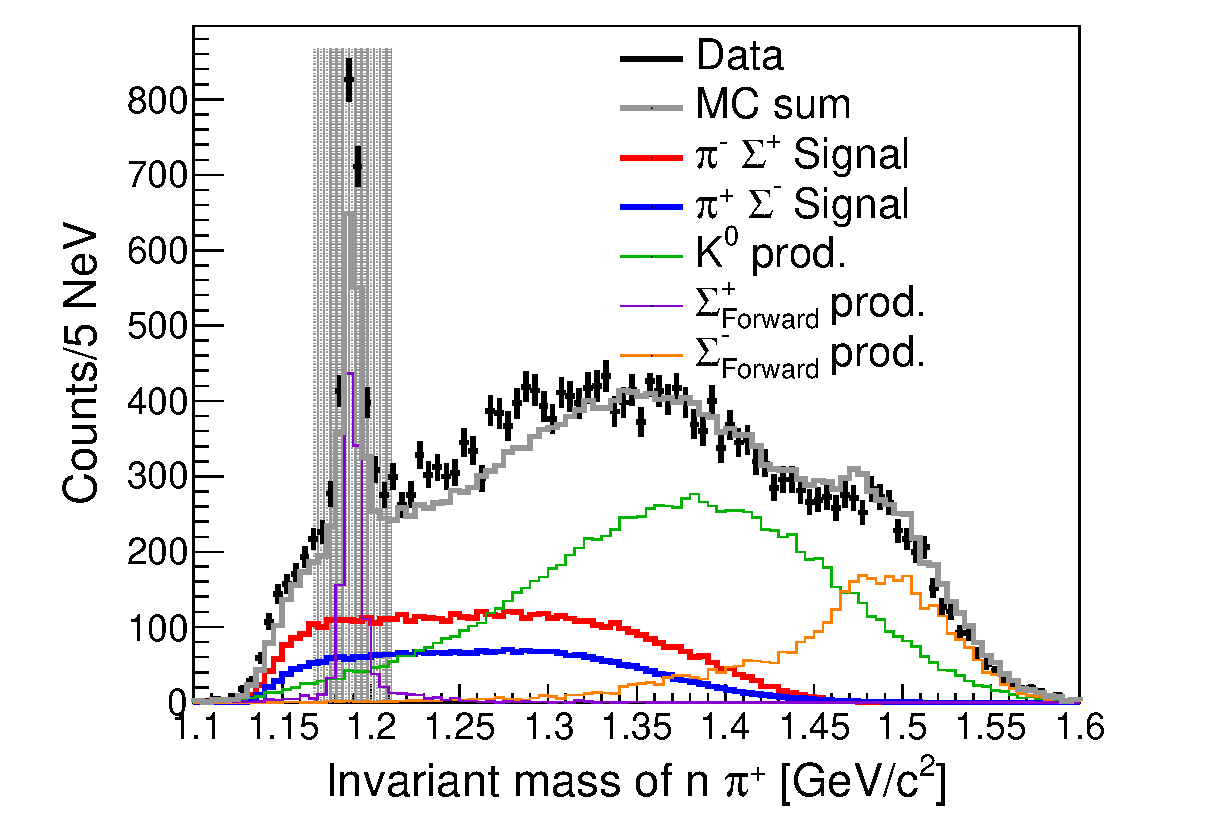
\includegraphics[width=4cm]{../pic/Dron/KN_ana/IM_npip.eps}
    \end{minipage}
  \end{tabular}
  \vspace{4mm}\\
  Each spectra are well reproduced. 
\end{frame}

\begin{figure}[htbp]
  \centering
  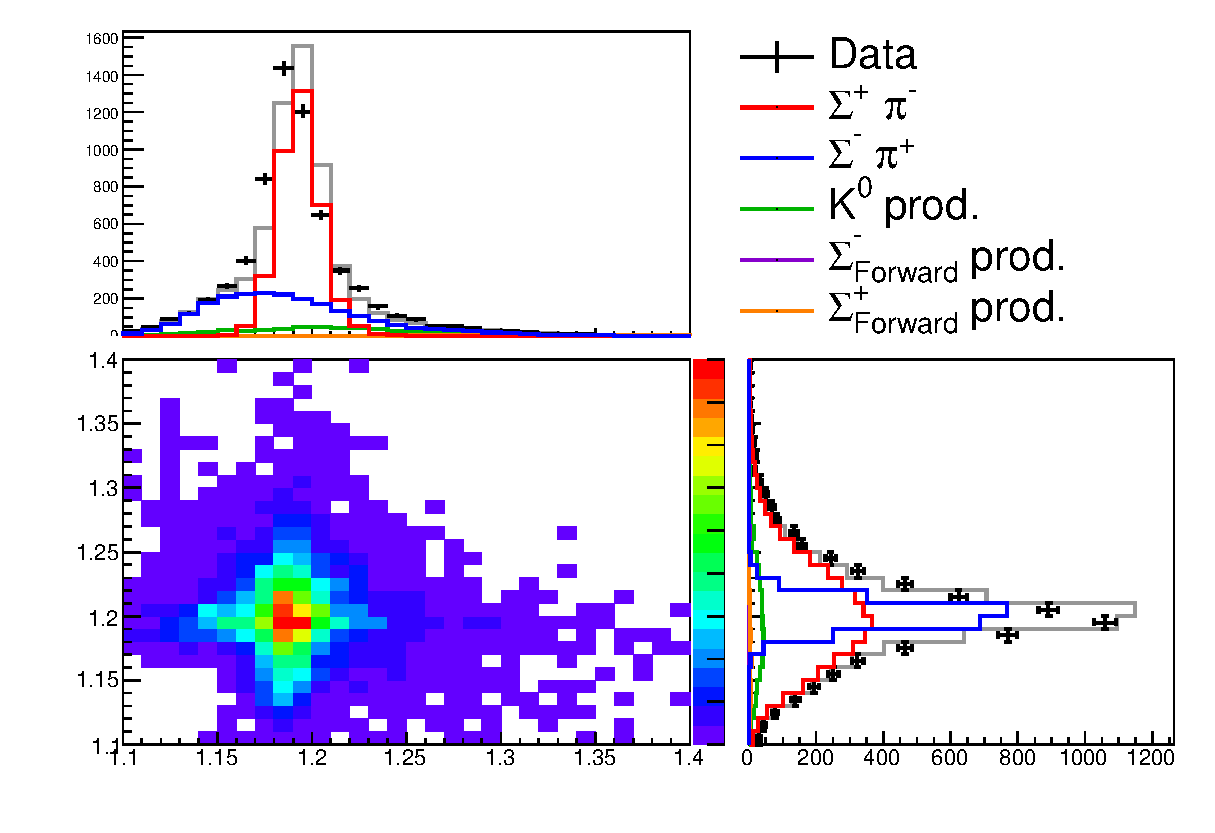
\includegraphics[width=12cm]{../pic/Run78/KN_ana_NC170_2sigma/KNpim_KNpip_MM.eps}
  \caption{
    This figure shows template fitting of the $d(K^-, n \pi)$ spectra to separate the $\pi^-\Sigma^+$ and $\pi^+ \Sigma^-$ modes.
    The lower left figure shows two-dimensional plots of $d(K^-, n \pi^-)$ and $d(K^-, n \pi^+)$ on the horizontal and vertical axes, respectively.
    The top and right panels show the projections onto each axis.
    The caption is the same as that of Figure.\ref{fig:fit_IM}.
  }
  \label{fig:fit_KNpi_MM_all}
\end{figure}


In this subsection, we explain procedure of template fitting, whose main purpose is decomposition of $\pi^- \Sigma^+$ and $\pi^+ \Sigma^-$ modes.
Template fitting is divided into two stages, one fitting to estimate the amount of background for $K^0$ and $\Sigma_{forward}$ production,
the other to separate $\pi^-\Sigma^+$ and $\pi^+\Sigma^-$ modes.
These fittings are performed using fitting with the likelihood method on a finite sample generated by Monte Carlo method\cite{temp_fit}.
There is no $\chi^2$ in this fitting,
but there is a value of $-2\log\Lambda$ that asymptotically approaches the $\chi^2$ when the number of samples become infinite, and the fitting is evaluated with this value.
Here, $\Lambda$ is the likelihood.

The first fitting is performed using the invariant mass distributions of $\pi^+ \pi^-$, $n \pi^+$ and $n \pi^-$ in the event that $K^-d \rightarrow n \pi^+ \pi^- n$ final state.
The $K^0$, $\Sigma^+$ and $\Sigma^-$ productions create peaks in the respective invariant mass distributions as shown in Fig.\ref{fig:fit_IM}.
The distributions reconstructed by fitting are also plotted in the same figure.
The bold line represents the case of backward $\pi \Sigma$ production of signal, with red and blue representing the $\pi^- \Sigma^+$ and $\pi^-\Sigma^+$ modes, respectively.
The other green, purple and orange lines represent the background for $K^0$, $\Sigma^-_{forward}$ and $\Sigma^+_{forward}$ production, respectively.
This fitting of $-2\log\Lambda$ is \IMfitChiSquare.
Degrees freedom is the number of bin with data, and $-2\log\Lambda/NDF \sim $\IMfitChiNDF. 
% For this purpose, the distribution is fitted with a Gaussian and a 5-th polynomial function, and the rejection region is defined by the 3$\sigma$ of the Gaussian.

\begin{figure}
  \begin{tabular}{ccccc}
    \begin{minipage}{0.2\hsize}
      \includegraphics[width=2.2cm]{../pic/Run78/KN_ana_NC170_2sigma/KNpi_MM_0.eps}
    \end{minipage}
    \begin{minipage}{0.2\hsize}
      \includegraphics[width=2.2cm]{../pic/Run78/KN_ana_NC170_2sigma/KNpi_MM_1.eps}
    \end{minipage}
    \begin{minipage}{0.2\hsize}
      \includegraphics[width=2.2cm]{../pic/Run78/KN_ana_NC170_2sigma/KNpi_MM_2.eps}
    \end{minipage}
    \begin{minipage}{0.2\hsize}
      \includegraphics[width=2.2cm]{../pic/Run78/KN_ana_NC170_2sigma/KNpi_MM_3.eps}
    \end{minipage}
    \begin{minipage}{0.2\hsize}
      \includegraphics[width=2.2cm]{../pic/Run78/KN_ana_NC170_2sigma/KNpi_MM_4.eps}
    \end{minipage}
  \end{tabular}
  \begin{tabular}{ccccc}
    \begin{minipage}{0.2\hsize}
      \includegraphics[width=2.2cm]{../pic/Run78/KN_ana_NC170_2sigma/KNpi_MM_5.eps}
    \end{minipage}
    \begin{minipage}{0.2\hsize}
      \includegraphics[width=2.2cm]{../pic/Run78/KN_ana_NC170_2sigma/KNpi_MM_6.eps}
    \end{minipage}
    \begin{minipage}{0.2\hsize}
      \includegraphics[width=2.2cm]{../pic/Run78/KN_ana_NC170_2sigma/KNpi_MM_7.eps}
    \end{minipage}
    \begin{minipage}{0.2\hsize}
      \includegraphics[width=2.2cm]{../pic/Run78/KN_ana_NC170_2sigma/KNpi_MM_8.eps}
    \end{minipage}
    \begin{minipage}{0.2\hsize}
      \includegraphics[width=2.2cm]{../pic/Run78/KN_ana_NC170_2sigma/KNpi_MM_9.eps}
    \end{minipage}
  \end{tabular}
  \begin{tabular}{ccccc}
    \begin{minipage}{0.2\hsize}
      \includegraphics[width=2.2cm]{../pic/Run78/KN_ana_NC170_2sigma/KNpi_MM_10.eps}
    \end{minipage}
    \begin{minipage}{0.2\hsize}
      \includegraphics[width=2.2cm]{../pic/Run78/KN_ana_NC170_2sigma/KNpi_MM_11.eps}
    \end{minipage}
    \begin{minipage}{0.2\hsize}
      \includegraphics[width=2.2cm]{../pic/Run78/KN_ana_NC170_2sigma/KNpi_MM_12.eps}
    \end{minipage}
    \begin{minipage}{0.2\hsize}
      \includegraphics[width=2.2cm]{../pic/Run78/KN_ana_NC170_2sigma/KNpi_MM_13.eps}
    \end{minipage}
    \begin{minipage}{0.2\hsize}
      \includegraphics[width=2.2cm]{../pic/Run78/KN_ana_NC170_2sigma/KNpi_MM_14.eps}
    \end{minipage}
  \end{tabular}
  \begin{tabular}{ccccc}
    \begin{minipage}{0.2\hsize}
      \includegraphics[width=2.2cm]{../pic/Run78/KN_ana_NC170_2sigma/KNpi_MM_15.eps}
    \end{minipage}
    \begin{minipage}{0.2\hsize}
      \includegraphics[width=2.2cm]{../pic/Run78/KN_ana_NC170_2sigma/KNpi_MM_16.eps}
    \end{minipage}
    \begin{minipage}{0.2\hsize}
      \includegraphics[width=2.2cm]{../pic/Run78/KN_ana_NC170_2sigma/KNpi_MM_17.eps}
    \end{minipage}
    \begin{minipage}{0.2\hsize}
      \includegraphics[width=2.2cm]{../pic/Run78/KN_ana_NC170_2sigma/KNpi_MM_18.eps}
    \end{minipage}
    \begin{minipage}{0.2\hsize}
      \includegraphics[width=2.2cm]{../pic/Run78/KN_ana_NC170_2sigma/KNpi_MM_19.eps}
    \end{minipage}
  \end{tabular}
  \begin{tabular}{ccccc}
    \begin{minipage}{0.2\hsize}
      \includegraphics[width=2.2cm]{../pic/Run78/KN_ana_NC170_2sigma/KNpi_MM_20.eps}
    \end{minipage}
    \begin{minipage}{0.2\hsize}
      \includegraphics[width=2.2cm]{../pic/Run78/KN_ana_NC170_2sigma/KNpi_MM_21.eps}
    \end{minipage}
    \begin{minipage}{0.2\hsize}
      \includegraphics[width=2.2cm]{../pic/Run78/KN_ana_NC170_2sigma/KNpi_MM_22.eps}
    \end{minipage}
    \begin{minipage}{0.2\hsize}
      \includegraphics[width=2.2cm]{../pic/Run78/KN_ana_NC170_2sigma/KNpi_MM_23.eps}
    \end{minipage}
    \begin{minipage}{0.2\hsize}
      \includegraphics[width=2.2cm]{../pic/Run78/KN_ana_NC170_2sigma/KNpi_MM_24.eps}
    \end{minipage}
  \end{tabular}
  \label{fig:fit_KNpi_MM}
  \caption{
    These figures are presented separately for each bin of $d(K^-, n)$ for fitting to separate $\pi^- \Sigma^+$ and $\pi^+ \Sigma^-$ modes.
    The top left figure shows the lowest missing mass in the $1.35$-$1.36$GeV bin, with the next bin represented as one goes to the right.
    In other words, one row is shown for the 0.05GeV region.
  }
\end{figure}

\begin{figure}[htbp]
  \centering

  \includegraphics[width=8cm]{../pic/Dron/tempFit_KNpi_MM_Chi2.eps}
  \caption{
    This figure shows the template fitting $-2\log\Lambda$ and $-2\log\Lambda/NDF$ for the separation of $\pi^- \Sigma^+$ and $\pi^+ \Sigma^-$ modes in each $d(K^-, n)$ bin.
    Black and red indicate $-2\log\Lambda$ and $-2\log\Lambda/NDF$, respectively.
    The horizontal axis is represented for $d(K^-, n)$ bins.
  }
  \label{fig:tempFit_KNpi_Chi2}
\end{figure}


The fitting to separate the $\pi^-\Sigma^+$ and $\pi^+\Sigma^-$ modes is performed for events from $K^-- d \rightarrow n \pi^+ \pi- n$, excluding $K^0 $and $\Sigma^{\pm}_{forward}$ production.
However, the background leakage is estimated by scaling the distribution reconstructed in the MC simulation by the intensity estimated by the invariant mass fitting.
This fitting is performed each bin of the missing mass of $d(K^-, n)$, since the scattering amplitude of $\bar{K}N \rightarrow \pi \Sigma$ depends on the $\pi \Sigma$ invariant mass.
For this fitting we use the $d(K^-, n \pi^-)$ and $d(K^-, n \pi^+)$ missing masses as shown in Fig.\ref{fig:fit_KNpi_MM_all}.
This figure shows the sum of the $d(K^- , n)$ bins.
The bottom left figure shows a two-dimensional figure of the $d(K^-, n \pi^-)$ and $d(K^-, n \pi^+)$ missing masses on the horizontal and vertical axes, respectively.
The top and right figures show the projections of the respective axes.
The missing mass of $d(K^-, n \pi)$ makes a peak at $\Sigma$ for the correct combination for the missing $\Sigma$, but is widely distributed in the kinematic region for the opposite charge.
For example, for $d(K^-, n \pi^-)$, the $\pi^- \Sigma^+$ mode has a peak structure as shown by the red line,
whereas the $\pi^+ \Sigma^-$ mode has a widely distributed structure as shown by the blue line.

Fig.\ref{fig:fit_KNpi_MM} shows the results for the fitting of each bin of $d(K^-, n)$ separately.
Fig.\ref{fig:tempFit_KNpi_Chi2} shows the $-2\log\Lambda$ and $-2\log\Lambda/NDF$ of this fitting in each $d(K^-, n)$ bin in black and red, respectively.

Fitting to estimate background and to separate $\pi^- \Sigma^+$ and $\pi^+ \Sigma^-$ modes cannot be performed simultaneously as they use different event samples.
They are therefore repeated in the following steps.

First, the separation of $\pi^- \Sigma^+$ and $\pi^+ \Sigma^-$ modes is performed without considering the background.
The obtained distribution of backward $\pi^{\mp} \Sigma^{\pm}$ modes is used for fitting to estimate the background,
which is then fed back into the fitting of the separation of $\pi^- \Sigma^+$ and $\pi^+ \Sigma^-$ modes.
After five iterations of this procedure, fitting is performed considering 2-step and direct $\Lambda(1520)$ generation for $K^0$ generation, which is described in the Appendix.\ref{apendix:K0_event}.
Finally, fitting of the separation of the $\pi^- \Sigma^+$ and $\pi^+ \Sigma^-$ modes is performed to obtain the final $\pi \Sigma$ spectrum as shown in Fig.\ref{fig:piS_num}..

\begin{figure}[htbp]
  \centering
  
  \includegraphics[width=8cm]{../pic/Dron/piS_num.eps}
  \caption{
    The $\pi^-\Sigma^+$ and $\pi^+\Sigma^-$ mode spectra obtained by template fitting are shown in arbitrary units.
    Red and blue lines indicate $\pi^-\Sigma^+$ and $\pi^+\Sigma^-$, respectively.
    The green vertical line is indicated the $\bar{K}N$ threshold.        
  }
  \label{fig:piS_num}
\end{figure}



%% \begin{frame}{Template fitting to decompose $K^0$ production}
  \begin{figure}
    \centering
    Invariant mass of $n K^0$\\
    \includegraphics[width=7.5cm]{../pic/Dron/K0_ana/npipi_IM_K0.eps}
  \end{figure}
  \centering
  2-step like component is seen about 11.5\%.\\
  Direct-$\Lambda(1520)$ prod. is seen about 7.7\%.\\
\end{frame}




\section{Conversion to the cross section}
\section{Conversion spectra to cross sections}
\begin{figure}[htbp]
  \centering
  \includegraphics[width=8cm]{../pic/Dron/KN_ana/kn_acc.eps}
  \caption{
    This figure shows the acceptance of $d(K^-, n)"\pi^{\mp}\Sigma^{\pm}"$.
    The red line indicates $\pi^- \Sigma^+$ and the blue line indicates $\pi^+ \Sigma^-$.
  }
  \label{fig:kn_acc}
\end{figure}

\begin{figure}[htbp]
  \centering
  \includegraphics[width=8cm]{../pic/Dron/KP_ana/kp_acc.eps}
  \caption{
    This figure shows $d(K^-, p)"\pi^-\Sigma^0"$ acceptance
  }
  \label{fig:kp_acc}
\end{figure}


This section describes the CDS acceptance correction.
For this correction, we use Monte Carlo simulation data for the $K^-d \rightarrow n \Lambda(1405)$, assuming a 2-step process,
which was also used for the template fitting in the previous section.
The CDS acceptance correction is applied not only to $d(K^-, n)\Lambda(1405)$ but also to $d(K^-, p)\Sigma^*$.
The simulation data for this correction were generated in the same way as for the $K^-d \rightarrow n \Lambda(1405)$ reaction.

The forward-going neutrons (protons) are generated with a slightly wider angular distribution (<8 degrees)
than the acceptance of the forward detector system.
However, since the purpose here is to estimate the CDS acceptance,
only the events that are detected by the forward detector are considered as the sample population.
Among these events, those that pass through the same analysis routine as the real data are regarded as valid events.
In the case of forward neutrons, the analysis includes events in which $\pi^+ \pi^-$ are detected,
followed by the selection of $d(K^-, n \pi^+ \pi^-)n$ events, and the rejection of $K^0$ and $\Sigma^{\pm}_{forward}$.
In the case of forward protons, valid events are those in which $\pi^- \pi^-$ are detected,
and are classified through the $d(K^-, p \pi^- \pi^-)\gamma p$ and $d(K^-, p \pi^-)\Lambda$ selections.

The CDS acceptances obtained for $d(K^-, n)\pi^{\mp}\Sigma^{\pm}$ and $d(K^-, p)\pi^-\Sigma^0$ are shown
in Figures \ref{fig:kn_acc} and \ref{fig:kp_acc}, respectively.



%% The acceptance of $d(K^-,n)"\pi^{\mp}\Sigma^{\pm}"$ and $d(K^-,p)"\pi^-\Sigma^0$ is corrected by MC simulations
%% in which nucleons are injected at a forward angle into the covered region of a forward detector with a uniform $\pi\Sigma$ mass distribution.
%% Since the solid angle of the forward detector is evaluated as subsection.\ref{subsec.XXX}, we adapt as the denominator the events for which the forward detector is analyzable.
%% The same analysis procedure as for the real data is applied to the MC simulation, and the final survival rate is evaluated and used as the acceptance.
%% That is, for $d(K^-, n)"\pi^{\mp}\Sigma^{\pm}"$, we apply $d(K^-, n \pi^+ \pi^-)"n"$ final state selection and rejection of $K^0$ and $\Sigma_{forward}$.
%% For $d(K^-, p)"\pi^-\Sigma^0"$, we apply the $d(K^-, p \pi^- \pi^-)"p \gamma"$ and $d(K^-, p \pi^-)"\Sigma^0"$ selections.
%% Fig.\ref{fig:kn_acc} shows the acceptance of $d(K^-, n)\pi^{\mp} \Sigma^{\pm}$.
%% Dents above the $\bar{K}N$ threshold are due to $K^0$ rejection.
%% The difference in absolute values between $\pi^- \Sigma^+$ and $\pi^+ \Sigma^-$ is due to the branching ratio of the $\Sigma$ decay.
%% Fig.\ref{fig:kp_acc} shows the acceptance of $d(K^-, p)"\pi^-\Sigma^0"$.

%% \begin{frame}{$K^0 cos\theta$ vs mom  {\bf Data}}
  \begin{tabular}{cc}
    \begin{minipage}{0.5\hsize}
      \begin{figure}
        Raw\\
        \includegraphics[width=6cm]{../pic/Run78/QE/K0_cos_mom_data.eps}
      \end{figure}
    \end{minipage}

    \begin{minipage}{0.5\hsize}
      \begin{figure}
        $Data(\cos_{K^0}, p_{K^0}))/A(\cos\theta_{K^0}, p_{K^0})$\\
%%        Accpectance corrected\\
        \includegraphics[width=6cm]{../pic/Run78/QE/K0_cos_mom_data_corr.eps}
      \end{figure}
    \end{minipage}
  \end{tabular}
  
  \centering

  Acceptance was presented at page.4
  
\end{frame}

%% \subsection{The spectrum of the $d(K^-, n)"n K^0"$}

\begin{figure}
  \centering
  \begin{tabular}{cc}
    \begin{minipage}{0.6\hsize}
      \includegraphics[width=7cm]{../pic/Run78/QE/KN_MM_wK0_tag.eps}
    \end{minipage}
    \begin{minipage}{0.4\hsize}
      \includegraphics[width=4cm]{../pic/Run78/QE/IM_pipi.eps}
    \end{minipage}
  \end{tabular}
  \caption{
    Right figure shows $K^0$ selection region and estimated background events which is zoom up of left figure of Fig\ref{fig:IM_fit}.
    Red lines indicate selection region.
    left figure shows $d(K^-, n)"n K^0"$ spectra with esmated backgrounds by MC template.
  }
  \label{fig:KN_MM_K0}
\end{figure}

Although the reaction can not measured below the $\bar{K}N$ threshold, 
in the $K^0$ take the strangeness, 
so these events are one of the strongest candidate of the prove for 1-step reaction strength of the $K^-N\rightarrow \bar{K}n$ reaction.\\
The backgrounds were estimated using the template fitting result which was shown in the right figure of Fit\ref{fig:KN_MM_K0}.
The background spectra shape of the $d(K^-, n)"n K^0"$ was indicated in the left figure of the same figure.
These spectra will be collected by the acceptance of the CDS using	the $K^0$ kinematics because detected particles by the CDS came from the $K^0$ decay.
The $K^0$ kinematics was represented as 2 variables function about the $\cos\theta$ and the absolute momentum value and
the acceptance of the CDS was collected event-by-event using the acceptance as weight function as the following equation.

\begin{equation}
  N_{corr}(m_{n K^0}) = \sum N(m_{n K^0}, \cos\theta_{K^0}, p_{K^0}) \cdot \frac{1}{A(\cos\theta_{K^0}, p_{K^0})} \label{eq:corr_K0} 
\end{equation}

\begin{figure}[htbp]
  \centering
  \includegraphics[width=7cm]{../pic/Run78/QE/K0_cos_mom_acc.eps}
  \caption{
    This figure shows the acceptance of the $K^-d\rightarrow K^0 n n$ reaction which was estimated by the Monte Calro simulation.
  }
  \label{fig:K0_acc}
\end{figure}

\begin{figure}[htbp]
  \centering
  \begin{tabular}{cc}
    \begin{minipage}{0.5\hsize}
      \includegraphics[width=7cm]{../pic/Run78/QE/K0_cos_mom_data.eps}
    \end{minipage}

    \begin{minipage}{0.5\hsize}
      \includegraphics[width=7cm]{../pic/Run78/QE/K0_cos_mom_BG.eps}
    \end{minipage}
  \end{tabular}
  \caption{
    These figure shows about $K^0$ emit angle and momentum in the experimental frame.
    Left figure shows about data and right figure shows background estimated by the Monte Calro.
  }
  \label{fig:K0_cos_mom}
\end{figure}

For this collection, the acceptance was estimated using the $K^- d \rightarrow n_{forwad} (K^0 n)$ reaction.
The mass of the $n K^0$ was generated flat distribution from the $K^0 n$ mass threshold to the kinematical threshold
to accumulate widely and isotropically acceptance which was shown in Fig\ref{fig:K0_acc}
This acceptance collection was adopted to the signal and the backgrounds.
Fig\ref{fig:K0_cos_mom} shows the $K^0$ kinmatics distribution about the data and the backgrounds estimated by the MC sim.
By this operation, we obtained the acceptance collected spectra as shown in Fig\ref{fig:KN_MM_K0_corr}.
Because the data distribution located at the edge of the acceptance and the backgrounds widely distributed, in the acceptance corrected spectra, the signal was enhanced.

\begin{figure}[htbp]
  \centering
  \includegraphics[width=8cm]{../pic/Run78/QE/K0_spec_wBG.eps}
  \caption{
    This figure shows acceptance corrected spectrum of the $d(K^-, n)"n K^0"$.
    Black line indicates data and color plots indicate the background reproduced by the Monte Calro simulation.
  }
  \label{fig:KN_MM_K0_corr}
\end{figure}


%% For $K^0$ production events, we use acceptance for $K^0$ kinematics because all detected particles are of $K^0$ origin.
%% We estimate the two-dimensional acceptances for $K^0$ momentum and $K^0$ scattering angles as shown in Fig\ref{fig.K0_cos_mom_acc}, and weight each event to correct for acceptances.
%% Fig.\ref{fig:K0_spec} shows acceptance corrected spectra of $K^0$ production with reproduced BG by MC simulations.
%% It can be seen that the data are concentrated in the backward and high momentum regions where the acceptances are small,
%% while the MC is distributed over the whole region as shown in Fig.\ref{fig:K0_cos_mom}.
%% In other words, the acceptance correction suppresses BG and emphasizes true $K^0$ production.

\subsection{$d(K^-, n)$ scaling factor}
$d(K^-, n)"X"$ spectrum can be converted from counts to the differential cross section ($\frac{d^2\sigma}{d\Omega dm}$) excepting the acceptance of the the CDS that is depend on the reaction.
The parameters was used for the conversion were summarized in Table\ref{tab:KN_scale}.

First one is luminosity which was consist of number of target, number of irradiated kaon, DAQ live rate, trigger efficeincy.
The number of target was defined from length of fiducial volume ($10cm$) and target density which was evaluated from measured tempature.
The number of irradiated kaon was defined by correcting kaon number counted up by the scaler DAQ by ratio of true kaon in kaon trigger which was described in Sec\ref{sec:beam_line_ana}.
About DAQ live rate and trigger efficiency were discribed in Sec\ref{sec:trigger}.
The luminosity was evaluated run-by-run.
In the table, these items were represented value weighted by data statistics as typical value.

Next is about the CDS which was CDC efficiency discribed in Sec\ref{sec:CDC_eff}.
Accpectances of CDS were estimated and corrected by the Monte Carlo simulation data.
These evaluations were described in individual section for each reactions.

Last one is about the NC which was consists of acceptance and efficiency.
The efficiency of the NC was further decomposed to intrinsic one and overveto by the CVC and the BVC that was described in Sec\ref{sec:NC_eff}.
The acceptance of the NC was estimated from the NC position and the error was evaluated from difference of the first layer and the last layer of the NC.

\input{analysis/KN_scaling_table}


\begin{table}
  \caption{
    Summary table of $d(K^-, p)$ scaling parameters
  }

  \hspace{-2cm}
  \begin{tabular}{cc|cc|cc}
    \multicolumn{2}{c|}{Component}  & value            & error           & value  & error \\
    \hline
    \hline
    Luminosity   ($/\mu b$)    &    & 2478             & 81          &  & \\
    & Target Length (cm)       &  & & 10               &                  \\
    & Target density $[g/cm^3]$&  & & 0.1624           & 0.0014           \\
    & Number of Kaon           &  & & 2.05$\times 10^{10}$ &              \\
    & Survival ratio of $K^-$  &  & & 0.336            & 0.0001           \\
    & DAQ live ratio           &  & & 0.821            & 0.0001           \\
    \multicolumn{2}{c|}{Trigger efficiency}  &  & &                  &    \\
    \hline
    & $K \otimes$CDH1          &  & & 0.9527           & 0.0003 \\
    & Charge                   &  & & 0.9559           & 0.0004 \\
    \hline
    \hline
    Efficiency of the CDC      &    & 0.977            & 0.04    &  & \\
    \hline
    %% \hline
    %% Acceptance of the PC/CVC (msr) & & \multicolumn{4}{|c}{Evaluate by the SIM} \\
    \hline
    Efficeincy of the forward detectors  &    & 0.819            & 0.042   &  & \\
    Efficeincy of the FDC1               &    & 0.987            & 0.005   &  & \\
  \end{tabular}
  \label{table:KP_scaling}
\end{table}


\begin{figure}[htbp]
  \centering
  \includegraphics[width=8cm]{../pic/Run78/KP_ana/solid_ang_144.eps}
  \caption{
    This figure shows the effective rates of solid angle elements in the 1.44–1.45 GeV $\pi^-\Sigma^0$ mass bin,
    as estimated by Monte Carlo simulations.
  }
  \label{fig:PCCVC_SA_elem}
\end{figure}

\begin{figure}[htbp]
  \centering
  \includegraphics[width=8cm]{../pic/Dron/PCCVC_SA.eps}
  \caption{
    This figure shows the relationship between the mass of the $\pi^-\Sigma^0$ system and
    the solid angles of the forward detectors (FDC1 and PC/CVC) with respect to the outgoing forward proton.
    The red line indicates the solid angle of the NC detector with respect to the forward neutron.
  }
  \label{fig:PCCVC_SA}
\end{figure}


The factors for converting to double-differential cross sections are explained here.
These can be categorized into the following three components:
\begin{enumerate}
\item Luminosity, which is determined by the number of incident beam particles and the number of target nuclei;
\item The solid angle and detection efficiency of the forward-scattered neutrons (or protons) produced in the reaction;
\item The detection efficiency of detectors.
\end{enumerate}

These are summarized in Tables \ref{table:KN_scaling} and \ref{table:KP_scaling} for the forward neutron and forward proton cases, respectively.

Luminosity is a quantity that represents the product of the number of incident beam particles and the number of target particles.
The beam intensity is evaluated by multiplying the beam scaler counts by the DAQ live ratio,
described in Section \ref{sec:DAQ_eff}, which accounts for the fraction of data actually recorded for analysis;
the trigger efficiency, described in Section \ref{sec:trig_eff}, which accounts for whether a trigger signal was actually generated;
and the fraction of $K^-$ beam triggers that passed through the fiducial volume of the target, as described in Section \ref{sec:beam_ana}.
This beam-related quantity is calculated and summed on a run-by-run basis.
Tables \ref{table:KN_scaling} and \ref{table:KP_scaling} show representative values
consisting of the average over all runs and the errors evaluated from the fluctuations.
For the number of target particles, the density of the liquid deuterium target is estimated from the monitored temperatures,
as described in Section \ref{sec:target} The uncertainty is evaluated based on fluctuations during the production run and
is calculated by multiplying the density by the length of the fiducial volume.

% The temperature of the liquid deuterium target is monitored, as described in Section \ref{sec:target},
% and this value is used to evaluate its density.

In the case of forward neutrons, since they travel in straight trajectories,
the solid angle can be defined by the area covered by the NC. When the solid angle is evaluated at the center of the NC
and the variation is assessed by shifting the evaluation point front and back, it is determined to be 21.5 $\pm$ 0.2 [msr]\%.
The detection efficiency of the neutron detector can be divided into two components
the intrinsic detection efficiency of the NC for neutrons and the over-veto effect by the CVC.
The intrinsic neutron detection efficiency is evaluated to be 31.7 $\pm$ 1.6 [\%] using the reaction
$K^- p \rightarrow K^0 n \rightarrow \pi^+ \pi^- n$ with a liquid hydrogen target, as described in Section \ref{sec:NC_eff}.
The over-veto effect in the CVC, which is also considered to be strongly influenced by beam-induced background,
is evaluated to be 8.1 $\pm$ 0.7 [\%] using the production run data, also described in Section \ref{sec:NC_overveto}.

In the case of forward protons, since they are bent by the Usniwaka magnet,
the solid angle coverage depends on the momentum of the forward-scattered proton, i.e., the mass of the $\pi^-\Sigma^0$ system.
To estimate this, we use a dataset similar to the Monte Carlo simulation used for the acceptance correction.
The solid angle for a given $\pi^-\Sigma^0$ mass region is evaluated by dividing the angular space into small solid angle elements.
For each element,
the detection efficiency of the forward detector system (CVC/PC) is evaluated based on whether the proton can actually be detected.
The effective solid angle for each element is then calculated by multiplying the element's solid angle by its detection efficiency,
as shown in Figure \ref{fig:PCCVC_SA_elem}
Finally, the total solid angle is obtained by summing these effective solid angles over all elements, as shown in Figure \ref{fig:PCCVC_SA}.
The solid angle does not change significantly in the region of interest.

In this data set, hadronic reactions and similar processes that could cause secondary interactions are turned off
to avoid double-counting losses already accounted for in the detection efficiency of forward protons evaluated in Section \ref{sec:PC_eff}.
Here, the detection efficiency of protons was estimated to be 81.9 $\pm$ 4.2 [\%] using the $K^- d \rightarrow \pi^- \pi^- p p$ reaction.
Also,
the detection efficiency of FDC1 was evaluated to be 98.7 $\pm$ 0.5 [\%] using the BVC as the trigger detector under the pion beam conditions,
as described in Section \ref{sec:FDC1_eff}.

After applying the CDS acceptance obtained in the previous subsection and the correction factors described here,
we obtain the $d(K^-, n)\pi^{\mp}\Sigma^{\pm}$ and $d(K^-, p)\pi^-\Sigma^0$ cross sections,
as shown in Figures \ref{fig:Charge_CS} and \ref{fig:pimS0_CS}, respectively.

% \begin{frame}{Cross Section of $d(K^-, n)"n K^0"$}
  \begin{figure}
    \includegraphics[width=8cm]{../pic/Run78/QE/K0_CS.eps}
  \end{figure}
  \centering
  Box indicates staticial errors.
%%  BG was subtracted.
\end{frame}

\begin{figure}[htbp]
  \centering
  \includegraphics[width=9cm]{../pic/Dron/KN_ana/ChargeCS.eps}
  \caption{
    The red figure and blue figure shows about $d(K^-, n)"\pi^+\Sigma^-"$ and $d(K^-, n)"\pi^-\Sigma^+"$, respectively.
    The inner frame (thin line), outer frame (thick line), and error bars represent the addition of statistical errors, fitting errors, and conversion errors, which were calculated by root-mean-square.
    The green vertical lines indicates $\bar{K}N$ threshold.
  }
  \label{fig:Charge_CS}
\end{figure}

\begin{figure}[htbp]
  \centering
  \includegraphics[width=9cm]{../pic/Dron/KP_ana/pimS0_CS.eps}
  \caption{
    This figure shows the cross section of $d(K^-, p)"\pi^- \Sigma^0"$.
    The box represents the statistical error, and the error bar represents the root mean squares of the conversion factor added to it.
    The green vertical lines indicates $\bar{K}N$ threshold.
  }
  \label{fig:pimS0_CS}
\end{figure}










%% The solid angle for a given $\pi^-\Sigma^0$ mass region is evaluated by summing the effective solid angles,
%% each weighted by the detection efficiency of the forward detector system (CVC/PC), over the solid angle bins of the generated protons.

%% In this data set, hadron reactions and other reactions are turned off to prevent double-counting of losses due to reactions included in the detection efficiency of forward protons evaluated in Section 2.3.


%% The obtained spectra are converted to cross sections.
%% For this purpose, the target, beam, and DAQ efficiencies are summarized as luminosity.
%% The target and beam quantities are discussed in Sections.\ref{sec:target} and \ref{sec:Kbeam}, respectively.
%% The DAQ efficiency consists of two parts, one of which is the DAQ live rate and the other is the trigger efficiency, described in Sections.\ref{sec:DAQ_live_rate} and \ref{sec:trigger}.
%% Detector efficiency is also evaluated and corrected for conversion to cross sections.
%% The CDC, NC, and PC efficiencies are described in Sections.\ref{sec:CDC}, \ref{sec:NC}, and \ref{sec:PC}, respectively. 
%% These conversion factors are common for the $\pi \Sigma$ spectra.
%% These factors are summarized in Table.\ref{table:KN_scaling} and Table.\ref{table:KP_scaling} about $d(K^-, n)$ and $d(K^-, p)$, respectively.

%% On the other hand, the acceptances depend on the $\pi \Sigma$ mass spectra.
%% % In the case of $d(K^-, n)"\pi^{\mp} \Sigma^{\pm}"$, the separation ratio of $\pi^- \Sigma^+$ and $\pi^+ \Sigma^-$ is also depend on.
%% We obtain the cross section of $d(K^-, n)"n K^0"$, $d(K-, n)"\pi^-\Sigma^0"$ and $d(K^-, p)"\pi^- \Sigma^0"$ by adapting the these corrections,
%% which are shown in Figure.\ref{fig:nK0_CS}, Figure.\ref{fig:Charge_CS}, and Figure.\ref{fig:pimS0_CS}, respectively.
%% We obtain the cross section of $d(K-, n)"\pi^-\Sigma^0"$ and $d(K^-, p)"\pi^- \Sigma^0"$ by adapting the these corrections,
%% which are shown in Fig.\ref{fig:Charge_CS}, and Fig.\ref{fig:pimS0_CS}, respectively.

% \begin{figure}[htbp]
  \centering
  \includegraphics[width=6cm]{../pic/Dron/K0_ana/K0_CS.eps}
  \caption{
    This figure shows the cross section of $d(K^-, n)"n K^0"$.
    The box represents the statistical error, and the error bar represents the root mean squares of the conversion factor added to it.
    The green vertical lines indicates $\bar{K}N$ threshold.
  }
  \label{fig:nK0_CS}
\end{figure}

\begin{figure}[htbp]
  \centering
  \includegraphics[width=6cm]{../pic/Dron/KN_ana/ChargeCS.eps}
  \caption{
    The red figure and blue figure shows about $d(K^-, n)"\pi^+\Sigma^-"$ and $d(K^-, n)"\pi^-\Sigma^+"$, respectively.
    The inner frame (thin line), outer frame (thick line), and error bars represent the addition of statistical errors, fitting errors, and conversion errors, which were calculated by root-mean-square.
    The green vertical lines indicates $\bar{K}N$ threshold.
  }
  \label{fig:ChargeCS}
\end{figure}

\begin{figure}[htbp]
  \centering
  \includegraphics[width=6cm]{../pic/Dron/KP_ana/pimS0_CS.eps}
  \caption{
    This figure shows the cross section of $d(K^-, p)"\pi^- \Sigma^0"$.
    The box represents the statistical error, and the error bar represents the root mean squares of the conversion factor added to it.
    The green vertical lines indicates $\bar{K}N$ threshold.
  }
  \label{fig:pimS0_CS}
\end{figure}


% We discuss the physical mean about obtained spectra.






\section{Spectra}
\subsection{Qualitative properties of obtained spectra}
\begin{figure}[htbp]
  \centering
  \includegraphics[width=8cm]{../pic/Dron/All_CS.eps}
  \caption{
    The obtained cross sections are plotted simultaneously in this figure.
    The $d(K^-, n)"\pi^-\Sigma^+$, $d(K^-, n)"\pi^+\Sigma^-"$, $d(K^-, n)"n K^0"$, and $d(K^-, p)"\pi^- \Sigma^0"$ plot as red, blue, green, and orange, lines respectively.
    The $d(K^-, n)"n K^0"$ is scaled to 1/10.
    The green virtical line indicates the $\bar{K}N$ threshold.
  }
  \label{fig:all_CS}
\end{figure}


The $d(K^-, n)\pi^{\mp}\Sigma^{\pm}$ and $d(K^-, p)\pi^-\Sigma^0$ spectra obtained through the procedures described in the previous section
are shown together in Figure \ref{fig:all_CS}.
In this figure, the green vertical line indicates the $\bar{K}N$ threshold.
This section discusses the qualitative features of the obtained spectra.

The experiment is interpreted as a two-step reaction, as described in Section \ref{sec:E31}.
The $\pi^-\Sigma^0$ spectrum contains only the $I=1$ component from the second-step scattering,
and this second-step scattering does not exhibit a significant structure, as there is no pole near the $\bar{K}N$ threshold.
As a result, the $\bar{K}N$ spectrum reflects the first-step scattering more directly.
A bump-like shape emerges from the $\bar{K}N$ threshold due to the Fermi motion of the spectator.

For the $I=0$ component, the second-step scattering is expected to exhibit a pronounced structure below the $\bar{K}N$ threshold
due to the presence of poles in that region.
This results in a spectral shape with a stronger enhancement below the $\bar{K}N$ threshold compared to the bump-like feature originating
from the first-step scattering.
Indeed, the observed $\pi^{\mp}\Sigma^{\pm}$ spectra, which contain both $I=0$ and $I=1$ components as well as their interference,
exhibit a clear structure below the $\bar{K}N$ threshold.
The overall spectral intensity is also larger than that of the $\pi^-\Sigma^0$ spectrum,
which only contains the $I=1$ component, due to the pole contribution in the $I=0$ channel.
The interference between the $I=0$ and $I=1$ components appears as a difference between the $\pi^-\Sigma^+$ and $\pi^+\Sigma^-$ spectra.
Since the measured spectra show a clear asymmetry between them,
the interference effect between $I=0$ and $I=1$ was observed in the reactions in this experiment.

In the second-step scattering near the $\bar{K}N$ threshold,
$S$-waves are expected to dominate due to the small angular momentum transfer transfer.
However, it is well known that in this region there are $I=0$ $D$-wave resonances, such as the $\Lambda(1520)$,
and $I=1$ $P$-wave resonances, such as the $\Sigma(1385)$.
The absence of structures around the $\Sigma(1385)$ region in the measured $I=1$ $\pi^-\Sigma^0$ spectrum,
as well as around both the $\Sigma(1385)$ and $\Lambda(1520)$ regions in the $\pi^+\Sigma^-$ and $\pi^-\Sigma^+$ spectra
with mixed $I=0$ and $I=1$ contributions, confirms that the $S$-wave dominates in the reactions observed in this experiment.


\subsection{Comparison with theoritical calculations}
\input{discussion/spectra/comp_theoritical_cacl}
\subsection{$\bar{K}N$ Pole parameters assuming the 2-step reaction} 
Next, we discuss the method for obtaining the $\bar{K}N$ pole parameters through fitting under the assumption of a 2-step reaction.
This approach is similar to that used by Noumi et el., as introduced in Chapter 1.
Since this analysis method focuses only on $I=0$, the obtained spectra are separated into components of $I=0$.
In this procedure, the spectra are further separated into components of $I=1$ and, in addition, the interference term between $I=0$ and $I=1$.
The obtained spectrum can be expressed as follows from the isospin relation.

\newcommand{\Tmat}{T_{\bar{K}N \rightarrow \pi \Sigma}}
\newcommand{\Cfirst}{C_{K^- N \rightarrow \bar{K}N}}
\newcommand{\CS}{\frac{d\sigma}{d\Omega dM}}
\begin{align}
  \CS(\pi^\mp \Sigma^\pm) \propto & \left| \Cfirst^0 \Tmat^{I=0} \mp \Cfirst^1 \Tmat^{I=1} \right|^2 \nonumber \\
  = & \left| \Cfirst^0 \Tmat^{I=0} \right|^2 + \left| \Cfirst^1 \Tmat^{I=1} \right|^2 \nonumber \\
    & \mp 2\mbox{Re}( \Cfirst^0 \Cfirst^1 \Tmat^{I=0} \Tmat^{I=1} ) & \label{eq:Charge_piS} \\
  \CS(\pi^- \Sigma^0) \propto & \left| \Cfirst^1 \Tmat^{I=1} \right|^2 \label{eq:pimS0}
\end{align}

Here, $\Tmat^{I=0,1}$ represents the $T$ matrix of the second $\bar{K}N \rightarrow \pi \Sigma$ scattering for isospin $I=0$ and $I=1$.
Additionally, $\Cfirst^{0,1}$ denotes the factor for the first $K^- p \rightarrow \bar{K}N$ scattering,
corresponding to the isospin $I=0$ and $I=1$ components of the second scattering.

Since it can be expressed as shown in Equation (\ref{eq:Charge_piS}), (\ref{eq:pimS0}),
the spectra corresponding to $I=0$, $I=1$, and their interference terms can be written as follows.
\begin{align}
  & \CS(I=0) \propto \frac{1}{2}\left( \CS(\pi^- \Sigma^+)+\CS(\pi^+ \Sigma^-)-\CS(\pi^-\Sigma^0) \right) \label{eq:I0}\\
  & \CS(I=1) \propto \CS(\pi^- \Sigma^0) \label{eq:I1}\\ 
  & \CS(int) \propto \left( \CS(\pi^- \Sigma^+)-\CS(\pi^+\Sigma^+) \right) \label{eq:interfer}
\end{align}

\begin{figure}[htbp]
  \centering
  \begin{tabular}{ccc}
    \begin{minipage}{0.33\hsize}
      \includegraphics[width=4cm]{../pic/Dron/fit_I0_KzeroN.eps}
    \end{minipage}
    \begin{minipage}{0.33\hsize}
      \includegraphics[width=4cm]{../pic/Dron/fit_I0_KN.eps}
    \end{minipage}
    \begin{minipage}{0.33\hsize}
      \includegraphics[width=4cm]{../pic/Dron/fit_I0_Kmp.eps}
    \end{minipage}
  \end{tabular}
  \begin{tabular}{ccc}
    \begin{minipage}{0.33\hsize}
      \includegraphics[width=4cm]{../pic/Dron/fit_scat_amp_I0_KzeroN.eps}
    \end{minipage}
    \begin{minipage}{0.33\hsize}
      \includegraphics[width=4cm]{../pic/Dron/fit_scat_amp_I0_KN.eps}
    \end{minipage}
    \begin{minipage}{0.33\hsize}
      \includegraphics[width=4cm]{../pic/Dron/fit_scat_amp_I0_Kmp.eps}
    \end{minipage}
  \end{tabular}
  \caption{
    This figure shows the $I=0$ spectrum obtained from Eq. (\ref{eq:I0}) and the fit results assuming a 2-step reaction.
    In the upper panel, the error bars represent the experimental data, the red line indicates the spectrum resulting from the fit,
    the solid line corresponds to the spectrum convolved with detector resolution, and the dashed line represents the spectrum without resolution.
    The lower panel displays the scattering amplitude for the two-step $\bar{K}N \rightarrow \bar{K}N$ scattering,
    where the red line indicates the real part and the blue line shows the imaginary part.
    The lines are the best-fit values and the bands hatched in color represent the width of the error due to fitting.
  }
  \label{fig:fit_2step_I0}
\end{figure}


The 2-step response can be expressed as follows,
\begin{equation*}
   \frac{d\sigma}{dM_{\pi\Sigma}d\Omega_{n}}
   =\left| \bra{n_{\theta=0}\pi\Sigma} T^2_{\bar{K}N_2 \rightarrow \pi \Sigma}
   G_0(\bar{K}, N_2) T^1_{K^-N_1 \rightarrow \bar{K} N} \ket{K^-\Phi_{d}} \right|^2 
\end{equation*}
where $G_0(\bar{K}, N_2)$, represents the Green's function describing the propagation of virtual $\bar{K}$ mesons
between the first and second scattering steps.
This equation can be factorized using the deuterium wavefunction $\psi_d(p)$ and decomposed into
a 1-step response $f_{res}(M_{\pi \Sigma})$function and a 2-step scattering amplitude as shown below.
\begin{align*}
   & \frac{d\sigma}{dM_{\pi\Sigma}d\Omega_{n}}
     \sim \left| T^2_{\bar{K}N_2 \rightarrow \pi \Sigma} \right|^2 F_{res}(M_{\pi \Sigma}) \\
   & F_{res}(M_{\pi \Sigma}) = \left| \int G_0(\bar{K}, N_2) T^1_{K^-N\rightarrow \bar{K}N} \psi_d(p) d^3p_{N} \right|^2
\end{align*}
The $T$-matrix of the second scattering is expressed as follows, utilizing the low-energy expansion up to the second order for the two channels
\cite{Lensniak}.
\begin{align*}
   & T^2_{\bar{K} N \rightarrow \bar{K}N} = \frac{A}{1-iA k_2+\frac{1}{2}A Rk_2^2}\\
   & T^2_{\bar{K} N \rightarrow \pi \Sigma} =
   \frac{e^{i\delta}}{\sqrt{k_1}}\frac{\sqrt{{\bf Im}A-\frac{1}{2}|A|^2{\bf Im}Rk_2^2}}{1-iAk_2+\frac{1}{2}ARk_2^2}
\end{align*}

This fit includes the scattering length $A$ and the effective range $R$ of the second-step scattering,
along with a parameter determining the overall scale.
In other words, the shape of the first-step scattering (reaction function) is fixed,
and the spectrum shape is determined solely by the second-step scattering.
The scattering length and effective range are complex numbers, so there are five free parameters in total.
This fitting is performed using three $\bar{K}N$ threshold values: $K^- p$, $\bar{K}N$ (the average of $K^- p$ and $K^0 n$), and $K^0 n$.
The discrepancies in the results arising from the differences in threshold values are evaluated as a source of systematic error.
These differences in threshold values are reflected not only in the mass of the $\bar{K}N$ channel in the $T$-matrix of the seccond-scattering
but also in the mass of the nucleon used to calculate the response function in the first-step scattering.
The figure above shows the results of the fit: black error bars represent the data,
and the red solid line shows the fit results convolved with detector resolution, which are used to calculate the chi-square.
The red dashed line shows the fit spectrum without detector resolution,
and the blue dashed line indicates the response function, scaled arbitrarily.
The figure below shows the scattering amplitude obtained from the fit, with red and blue representing the real and imaginary parts, respectively.
The lines indicate the best-fit result, and the bands show the error range,
determined by the maximum and minimum values when adjusting the real and imaginary parts of $A$ and $R$ within their error margins.
The central values of the parameters and the fitting errors were evaluated in terms of the average $\bar{K}N$ threshold,
with $A = \fitScatLength$ and $R = \fitEffRange$.
These values need to be converted to the pole’s position [MeV] and width [MeV],
where the pole is defined by setting the denominator of the $T$-matrix to zero, i.e., by solving the following equation.
\begin{equation}
\frac{1}{2}ARk^2+Ak^2+1=0 \label{eq:pole}
\end{equation}
Where $k$ is the momentum of the $\bar{K}N$ center-of-mass system, converted to mass by $m=\sqrt{m_{\bar{K}N}^2+k^2}$.

\begin{figure}
  \begin{tabular}{ccc}
    \begin{minipage}{0.33\hsize}
      \includegraphics[width=4cm]{../pic/Dron/fit_L1405_pole_Kmp_5.eps}
    \end{minipage}
    \begin{minipage}{0.33\hsize}
      \includegraphics[width=4cm]{../pic/Dron/fit_L1405_pole_KN_5.eps}
    \end{minipage}
    \begin{minipage}{0.33\hsize}
      \includegraphics[width=4cm]{../pic/Dron/fit_L1405_pole_KzeroN_5.eps}
    \end{minipage}
  \end{tabular}

  \begin{tabular}{ccc}
    \begin{minipage}{0.33\hsize}
      \includegraphics[width=4cm]{../pic/Dron/fit_L1405_pole_Kmp_4.eps}
    \end{minipage}
    \begin{minipage}{0.33\hsize}
      \includegraphics[width=4cm]{../pic/Dron/fit_L1405_pole_KN_4.eps}
    \end{minipage}
    \begin{minipage}{0.33\hsize}
      \includegraphics[width=4cm]{../pic/Dron/fit_L1405_pole_KzeroN_4.eps}
    \end{minipage}
  \end{tabular}

  \begin{tabular}{ccc}
    \begin{minipage}{0.33\hsize}
      \includegraphics[width=4cm]{../pic/Dron/fit_L1405_pole_Kmp_3.eps}
    \end{minipage}
    \begin{minipage}{0.33\hsize}
      \includegraphics[width=4cm]{../pic/Dron/fit_L1405_pole_KN_3.eps}
    \end{minipage}
    \begin{minipage}{0.33\hsize}
      \includegraphics[width=4cm]{../pic/Dron/fit_L1405_pole_KzeroN_3.eps}
    \end{minipage}
  \end{tabular}

  \begin{tabular}{ccc}
    \begin{minipage}{0.33\hsize}
      \includegraphics[width=4cm]{../pic/Dron/fit_L1405_pole_Kmp_2.eps}
    \end{minipage}
    \begin{minipage}{0.33\hsize}
      \includegraphics[width=4cm]{../pic/Dron/fit_L1405_pole_KN_2.eps}
    \end{minipage}
    \begin{minipage}{0.33\hsize}
      \includegraphics[width=4cm]{../pic/Dron/fit_L1405_pole_KzeroN_2.eps}
    \end{minipage}
  \end{tabular}

  \begin{tabular}{ccc}
    \begin{minipage}{0.33\hsize}
      \includegraphics[width=4cm]{../pic/Dron/fit_L1405_pole_Kmp_1.eps}
    \end{minipage}
    \begin{minipage}{0.33\hsize}
      \includegraphics[width=4cm]{../pic/Dron/fit_L1405_pole_KN_1.eps}
    \end{minipage}
    \begin{minipage}{0.33\hsize}
      \includegraphics[width=4cm]{../pic/Dron/fit_L1405_pole_KzeroN_1.eps}
    \end{minipage}
  \end{tabular}
  
  \begin{tabular}{ccc}
    \begin{minipage}{0.33\hsize}
      \includegraphics[width=4cm]{../pic/Dron/fit_L1405_pole_Kmp_0.eps}
    \end{minipage}
    \begin{minipage}{0.33\hsize}
      \includegraphics[width=4cm]{../pic/Dron/fit_L1405_pole_KN_0.eps}
    \end{minipage}
    \begin{minipage}{0.33\hsize}
      \includegraphics[width=4cm]{../pic/Dron/fit_L1405_pole_KzeroN_0.eps}
    \end{minipage}
  \end{tabular}
  
  \caption{
    This figure shows the distribution and fit of the poles of $\Lambda(1405)$, generated using Gaussian random numbers.
    The right, center, and left panels correspond to the results based on the $K^- p$, $\bar{K}N$, and $K^0 n$ thresholds, respectively.
    The top row represents the fit over the entire range,
    followed by rows corresponding to the equivalent ranges of $3\sigma$, $2.5\sigma$, $2\sigma$, $1.5\sigma$, and $1\sigma$.
    The fit results are shown as red lines, with gray hatched areas representing regions excluded from the fit.
    The green lines indicate the pole positions corresponding to the best-fit values shown in Figure \ref{fig:fit_2step_I0}.
  }
  \label{fig:fit_L1405_pole}
\end{figure}

\begin{figure}
  \begin{tabular}{ccc}
    \begin{minipage}{0.33\hsize}
      \includegraphics[width=4cm]{../pic/Dron/fit_L1405_width_Kmp_5.eps}
    \end{minipage}
    \begin{minipage}{0.33\hsize}
      \includegraphics[width=4cm]{../pic/Dron/fit_L1405_width_KN_5.eps}
    \end{minipage}
    \begin{minipage}{0.33\hsize}
      \includegraphics[width=4cm]{../pic/Dron/fit_L1405_width_KzeroN_5.eps}
    \end{minipage}
  \end{tabular}

  \begin{tabular}{ccc}
    \begin{minipage}{0.33\hsize}
      \includegraphics[width=4cm]{../pic/Dron/fit_L1405_width_Kmp_4.eps}
    \end{minipage}
    \begin{minipage}{0.33\hsize}
      \includegraphics[width=4cm]{../pic/Dron/fit_L1405_width_KN_4.eps}
    \end{minipage}
    \begin{minipage}{0.33\hsize}
      \includegraphics[width=4cm]{../pic/Dron/fit_L1405_width_KzeroN_4.eps}
    \end{minipage}
  \end{tabular}

  \begin{tabular}{ccc}
    \begin{minipage}{0.33\hsize}
      \includegraphics[width=4cm]{../pic/Dron/fit_L1405_width_Kmp_3.eps}
    \end{minipage}
    \begin{minipage}{0.33\hsize}
      \includegraphics[width=4cm]{../pic/Dron/fit_L1405_width_KN_3.eps}
    \end{minipage}
    \begin{minipage}{0.33\hsize}
      \includegraphics[width=4cm]{../pic/Dron/fit_L1405_width_KzeroN_3.eps}
    \end{minipage}
  \end{tabular}

  \begin{tabular}{ccc}
    \begin{minipage}{0.33\hsize}
      \includegraphics[width=4cm]{../pic/Dron/fit_L1405_width_Kmp_2.eps}
    \end{minipage}
    \begin{minipage}{0.33\hsize}
      \includegraphics[width=4cm]{../pic/Dron/fit_L1405_width_KN_2.eps}
    \end{minipage}
    \begin{minipage}{0.33\hsize}
      \includegraphics[width=4cm]{../pic/Dron/fit_L1405_width_KzeroN_2.eps}
    \end{minipage}
  \end{tabular}

  \begin{tabular}{ccc}
    \begin{minipage}{0.33\hsize}
      \includegraphics[width=4cm]{../pic/Dron/fit_L1405_width_Kmp_1.eps}
    \end{minipage}
    \begin{minipage}{0.33\hsize}
      \includegraphics[width=4cm]{../pic/Dron/fit_L1405_width_KN_1.eps}
    \end{minipage}
    \begin{minipage}{0.33\hsize}
      \includegraphics[width=4cm]{../pic/Dron/fit_L1405_width_KzeroN_1.eps}
    \end{minipage}
  \end{tabular}
  
  \begin{tabular}{ccc}
    \begin{minipage}{0.33\hsize}
      \includegraphics[width=4cm]{../pic/Dron/fit_L1405_width_Kmp_0.eps}
    \end{minipage}
    \begin{minipage}{0.33\hsize}
      \includegraphics[width=4cm]{../pic/Dron/fit_L1405_width_KN_0.eps}
    \end{minipage}
    \begin{minipage}{0.33\hsize}
      \includegraphics[width=4cm]{../pic/Dron/fit_L1405_width_KzeroN_0.eps}
    \end{minipage}
  \end{tabular}
  
  \caption{
    This figure shows the distribution and fit of the widths of $\Lambda(1405)$, generated using Gaussian random numbers.
    The details of the figure caption are identical to those of Figure \ref{fig:fit_L1405_pole}, which provides further context.
  }
  \label{fig:fit_L1405_width}
\end{figure}

\begin{figure}
  \begin{tabular}{cc}
    \begin{minipage}{0.5\hsize}
      \includegraphics[width=7cm]{../pic/Dron/L1405_pole_chi2NDF.eps}
    \end{minipage}
    \begin{minipage}{0.5\hsize}
      \includegraphics[width=7cm]{../pic/Dron/L1405_width_chi2NDF.eps}
    \end{minipage}
  \end{tabular}
  
  \caption{
    This figure illustrates the $\chi^2/NDF$ relationship for the fittings of the $Lambda(1405)$ pole and width,
    as shown in Figures \ref{fig:fit_L1405_pole} and \ref{fig:fit_L1405_width}.
    The left panel corresponds to the pole fittings, while the right panel represents the width fittings.
    The purple, red, and blue lines indicate the results for the $K^- p$, $\bar{K}N$, and $K^0n$ thresholds, respectively.
  }
  \label{fig:L1405_param_chi2NDF}
\end{figure}


Since $A$ and $R$ are complex numbers, propagating their errors is not straightforward.
Therefore, the position and width errors of the poles are estimated by generating a Gaussian distribution
using the real and imaginary parts of $A$ and $R$ as random variables,
with fitting errors as the standard deviation $\sigma$.
This approach is similar to the conventional error propagation method,
which treats each parameter as an independent Gaussian, with the overall error as a composite of Gaussian distributions.
Figure \ref{fig:fit_L1405_pole}, \ref{fig:fit_L1405_width} shows the resulting distribution of position and width.
These distributions are clearly asymmetric, particularly in terms of width, due to a threshold effect caused by the proximity of the thresholds.

\begin{equation*}
  f_{fit}(x)=
  \left\{
    \begin{array}{ll}
      A\exp \left( -\frac{(x-M)^2}{2\sigma_h^2} \right) & (x>M) \\
      A\exp \left( -\frac{(x-M)^2}{2\sigma_l^2} \right) & (x<M)
    \end{array}
  \right.
\end{equation*}

Here, $M$ represents the central value, with $\sigma_h$ and $\sigma_l$ denoting the errors in the high and low regions, respectively.
This function explicitly distinguishes between errors above and below the central value while ensuring continuity at $M$.
%% Here, $M$ represents the central value, with $\sigma_h$ and $\sigma_l$ denoting the errors in the high and low regions, respectively.
%% This function, therefore,
%% has distinct errors in the high and low regions relative to the central value and remains continuous at that central point.
The distribution includes a tail component that deviates from a Gaussian profile, which must be excluded for accurate error evaluation.
%The distribution also appears to include a so-called tail component, which deviates from a Gaussian profile,
% and this component should be excluded to properly evaluate the errors.
To achieve this, the evaluation range is divided into several regions, each corresponding to a percentage of the peak height,
and the fit is performed in each region.
For instance, $\exp\left(-\frac{1}{2}3^2\right)$ corresponds to the $\pm 3 \sigma$ region.
This fitting process was conducted for all regions, ranging from $3\sigma$ to $1\sigma$, with increments of $0.5\sigma$.
Figure \ref{fig:L1405_param_chi2NDF} shows the relationship between the reduced $\chi^2/NDF$ and the cut range for each fit.
Here, the $\chi^2/NDF$ increases from the entire region to $3\sigma$.
This is thought to be due to the limited improvement in the fit because the tail component was not fully removed,
as well as the decrease in $NDF$ resulting from the narrower range.
The $\chi^2/NDF$ seems to reach saturation at the $1.5\sigma$ range.
Therefore, a range of $1.5\sigma$ is chosen as a reference to determine the position and width of the pole of $\Lambda(1405)$,
which is found to be $\fitPole + [\fitWidth]i$ [MeV].
Here, the central value is determined from the scattering length and the effective range of the best fit.
The fitting errors are evaluated using the average of $K^0n$ and $K^-p$ for the threshold values,
and the systematic errors were assessed by varying the threshold values.




\subsection{Comparison with DCC model} 
Here, the spectra are decomposed into the $I=0$, $I=1$, and interference components in order to clarify the contriutions of these factors.
The obtained spectrum can be expressed as follows from the isospin relation.

\newcommand{\Tmat}{T_{\bar{K}N \rightarrow \pi \Sigma}}
\newcommand{\Cfirst}{C_{K^- N \rightarrow \bar{K}N}}
\newcommand{\CS}{\frac{d\sigma}{d\Omega dM}}
\begin{align}
  \CS(\pi^\mp \Sigma^\pm) \propto & \left| \Cfirst^0 \Tmat^{I=0} \mp \Cfirst^1 \Tmat^{I=1} \right|^2 \nonumber \\
  = & \left| \Cfirst^0 \Tmat^{I=0} \right|^2 + \left| \Cfirst^1 \Tmat^{I=1} \right|^2 \nonumber \\
    & \mp 2\mbox{Re}( \Cfirst^0 \Cfirst^1 \Tmat^{I=0} \Tmat^{I=1} ) & \label{eq:Charge_piS} \\
  \CS(\pi^- \Sigma^0) \propto & \left| \Cfirst^1 \Tmat^{I=1} \right|^2 \label{eq:pimS0}
\end{align}

Here, $\Tmat^{I=0,1}$ represents the $T$ matrix of the second $\bar{K}N \rightarrow \pi \Sigma$ scattering for isospin $I=0$ and $I=1$.
Additionally, $\Cfirst^{0,1}$ denotes the factor for the first $K^- p \rightarrow \bar{K}N$ scattering,
corresponding to the isospin $I=0$ and $I=1$ components of the second scattering.

Since it can be expressed as shown in Equation (\ref{eq:Charge_piS}), (\ref{eq:pimS0}),
the spectra corresponding to $I=0$, $I=1$, and their interference terms can be written as follows.
\begin{align}
   \CS(I=0) \propto & \frac{1}{2}\left( \CS(\pi^- \Sigma^+)+\CS(\pi^+ \Sigma^-)-\CS(\pi^-\Sigma^0) \right) \nonumber \\
            = & \left| \Cfirst^0 \Tmat^{I=0} \right|^2 \label{eq:I0}\\
   \CS(I=1) \propto & \CS(\pi^- \Sigma^0) \nonumber \\
            = & \left| \Cfirst^1 \Tmat^{I=1} \right|^2 \label{eq:I1}\\
   \CS(int) \propto & \left( \CS(\pi^- \Sigma^+)-\CS(\pi^+\Sigma^+) \right) \nonumber \\
            = & 4\mbox{Re}( \Cfirst^0 \Cfirst^2 \Tmat^{I=0} \Tmat^{I=1} ) \label{eq:interfer}
\end{align}

The spectrum is transformed according to this formula.
We introduce scaling parameters $S_{I=0}$ and $S_{I=1}$ to adjust the intensities of the $I=0$ and $I=1$ components,
respectively, so that the overall spectral shape becomes more comparable to the theoretical spectrum.
The interference terms are scaled by $\sqrt{S_{I=0}S_{I=1}}$, as described in Equation \ref{eq:interfer}.

\begin{figure}[htbp]
  \begin{tabular}{cc}
    \begin{minipage}{0.5\hsize}
      \centering
      \includegraphics[width=6.0cm]{../pic/Dron/fit_model_A_fix_Phi/I0_fit.eps}
    \end{minipage}

    \begin{minipage}{0.5\hsize}
      \centering
      \includegraphics[width=6.0cm]{../pic/Dron/fit_model_B_fix_Phi/I0_fit.eps}
    \end{minipage}
  \end{tabular}

  \begin{tabular}{cc}
    \begin{minipage}{0.5\hsize}
      \centering
      \includegraphics[width=6.0cm]{../pic/Dron/fit_model_A_fix_Phi/pimS0_fit.eps}
    \end{minipage}

    \begin{minipage}{0.5\hsize}
      \centering
      \includegraphics[width=6.0cm]{../pic/Dron/fit_model_B_fix_Phi/pimS0_fit.eps}
    \end{minipage}
  \end{tabular}

  \begin{tabular}{cc}
    \begin{minipage}{0.5\hsize}
      \centering
      \includegraphics[width=6.0cm]{../pic/Dron/fit_model_A_fix_Phi/interfer_fit.eps}
    \end{minipage}

    \begin{minipage}{0.5\hsize}
      \centering
      \includegraphics[width=6.0cm]{../pic/Dron/fit_model_B_fix_Phi/interfer_fit.eps}
    \end{minipage}
  \end{tabular}
  \caption{
    This figure illustrates the spectra of the experimental data, decomposed into $I=0$, $I=1$, their interference terms,
    and the corresponding fitting results obtained using Model A of the DCC model.
    The black error bars represent the experimental data, while the red line denotes the fit results.
    The upper-left panel corresponds to $I=0$, the upper-right panel to $I=1$, and the lower panel to the interference term.
  }
  \label{fig:fit_scale}
\end{figure}

\begin{table}[h]
  \caption{
    This table shows the pole position with $I=0$ and $J^P=1/2^-$ below the $\bar{K}N$ threshold by DCC models\cite{DCC2}
  }
  \centering
  \begin{tabular}{ccc}
    \hline
    \hline
    & pole1 & pole2 \\
    \hline
    Model.A & $1437-75i$ & $1372-56i$ \\
    Model.B & $1428-31i$ & $1397-98i$ \\
    \hline
    \hline
  \end{tabular}
  \label{table:DCC_poles}
\end{table}


By fitting with these parameters, we obtain $S_{I=0} = \fitAscaleIz$ and $S_{I=1} = \fitAscaleIo$ for Model A,
and $S_{I=0} = \fitBscaleIz$ and $S_{I=1} = \fitBscaleIo$ for Model B.
The results of these fits are shown in the Fig.\ref{fig:fit_scale} : the left panel corresponds to Model A, and the right panel to Model B.
The top subpanels show the spectra for the $I=0$ component, the middle ones for the $I=1$ component (i.e., the $\pi^-\Sigma^0$ spectrum),
and the bottom ones for the interference term.

In Model B (right panel), a reasonably good agreement is observed across all spectra.
In contrast, Model A (left panel) reproduces the central $I=1$ term well, but the upper $I=0$ and lower interference terms
appear to be underestimated in the fit results in the quasi-elastic scattering region.
Indeed, the $\chi^2/NDF$ values are $\fitBscaleChi = \fitBscaleChiNum$ for Model B and
$\fitAscaleChi = \fitAscaleChiNum$ for Model A, indicating a significantly better fit for Model B.
This discrepancy is considered to arise from the fact that the theoretical spectrum for $I=0$ possesses a long-tailed component in the bound region.
Table \ref{table:DCC_poles} summarizes the parameters of the $I=0$ pole used in the theoretical calculations for the fit.
This is attributed to the large imaginary part of pole 1,
which is strongly coupled to the $\bar{K}N$ channel and therefore has a pronounced effect in this experiment.

As shown in Eq.(\ref{eq:interfer}), the phase difference between $I=0$ and $I=1$ modifies the interference term.
We demonstrate that introducing this phase difference as a fitting parameter leads to an improved fit.
The following discussion focuses exclusively on Model B, which provided the better overall agreement.
Since the $I=1$ component is determined solely from the experimental spectrum, two fitting strategies can be considered
(i) first fixing the $I=1$ contribution by $\pi^- \Sigma^0$ spectrum, or (ii) fitting all spectra simultaneously.
The results obtained from these two approaches are presented in Fig. \ref{fig:fit_B_phase_fixI1} and \ref{fig:fit_B_phase}.



\begin{figure}[htbp]
  \begin{tabular}{cc}
    \begin{minipage}{0.5\hsize}
      \centering
      \includegraphics[width=6.0cm]{../pic/Dron/fit_model_B_2/I0_fit.eps}
    \end{minipage}

    \begin{minipage}{0.5\hsize}
      \centering
      \includegraphics[width=6.0cm]{../pic/Dron/fit_model_B_2/pimS0_fit.eps}
    \end{minipage}
  \end{tabular}

  \centering
  \includegraphics[width=6.0cm]{../pic/Dron/fit_model_B_2/interfer_fit.eps}
  \caption{
    This figure shows the fitting results obtained when the degrees of freedom associated with the interference term
    are introduced as additional fitting parameters.
    The upper-left panel displays the $I=0$ component, the upper-right panel shows the $I=1$ component,
    and the lower panel presents the spectrum of the interference term.
    The error bars denote the experimental data, while the blue curve represents the fit obtained using DCC Model B.
    In this figure, the $I=1$ strength is determind by the only $\pi^- \Sigma^0$ spectrum.
  }
  \label{fig:fit_B_phase_fixI1}
\end{figure}

\begin{figure}[htbp]
  \begin{tabular}{cc}
    \begin{minipage}{0.5\hsize}
      \centering
      \includegraphics[width=6.0cm]{../pic/Dron/fit_model_B/I0_fit.eps}
    \end{minipage}

    \begin{minipage}{0.5\hsize}
      \centering
      \includegraphics[width=6.0cm]{../pic/Dron/fit_model_B/pimS0_fit.eps}
    \end{minipage}
  \end{tabular}

  \centering
  \includegraphics[width=6.0cm]{../pic/Dron/fit_model_B/interfer_fit.eps}
  \caption{
    This figure shows the results of the fitting using Model.B with the introduction of parameters related to the interference term.
    The notation is the same as in Fig.\ref{fig:fit_B_scale}.
    All three parameters are determined simultaneously in this fitting.
  }
  \label{fig:fit_B_phase}
\end{figure}




% \section{Fitting assuming the 2-step reaction}

% \section{Fitting with DCC method}
% \begin{figure}[htbp]
  \centering
  \includegraphics[width=6cm]{../pic/Dron/K0_ana/K0_CS.eps}
  \caption{
    This figure shows the cross section of $d(K^-, n)"n K^0"$.
    The box represents the statistical error, and the error bar represents the root mean squares of the conversion factor added to it.
    The green vertical lines indicates $\bar{K}N$ threshold.
  }
  \label{fig:nK0_CS}
\end{figure}

\begin{figure}[htbp]
  \centering
  \includegraphics[width=6cm]{../pic/Dron/KN_ana/ChargeCS.eps}
  \caption{
    The red figure and blue figure shows about $d(K^-, n)"\pi^+\Sigma^-"$ and $d(K^-, n)"\pi^-\Sigma^+"$, respectively.
    The inner frame (thin line), outer frame (thick line), and error bars represent the addition of statistical errors, fitting errors, and conversion errors, which were calculated by root-mean-square.
    The green vertical lines indicates $\bar{K}N$ threshold.
  }
  \label{fig:ChargeCS}
\end{figure}

\begin{figure}[htbp]
  \centering
  \includegraphics[width=6cm]{../pic/Dron/KP_ana/pimS0_CS.eps}
  \caption{
    This figure shows the cross section of $d(K^-, p)"\pi^- \Sigma^0"$.
    The box represents the statistical error, and the error bar represents the root mean squares of the conversion factor added to it.
    The green vertical lines indicates $\bar{K}N$ threshold.
  }
  \label{fig:pimS0_CS}
\end{figure}



